\documentclass[11pt]{amsart}
\usepackage[margin=1in]{geometry}
\usepackage{amsmath,amssymb,amsthm,mathtools,booktabs}
\usepackage{enumitem}
\usepackage{hyperref}
\hypersetup{colorlinks=true,linkcolor=blue,citecolor=blue,urlcolor=blue}
% \usepackage[final]{microtype}  % Removed for compilation compatibility; microtypographic features optional for journal submission
\usepackage[table]{xcolor}
\usepackage{array}
\usepackage{tabularx}
\usepackage{xurl}
\urlstyle{same}
\usepackage{pgfplots}
\pgfplotsset{compat=1.18}
\usepackage{tikz}
\usetikzlibrary{arrows.meta,positioning,fit,shapes.geometric,calc}
% \emergencestretch setting removed for compatibility in current build environment.

\newcommand{\leanrepo}{https://github.com/HQIV/hqiv-lean/blob/main}
\newcommand{\scriptrepo}{https://github.com/HQIV/hqiv-lean/blob/main/scripts}
\newcommand{\leanid}[1]{{\footnotesize\path{#1}}}
\newcommand{\leanfile}[1]{\href{\leanrepo/#1}{\footnotesize\path{#1}}}
\newcommand{\scriptbundle}[1]{\path{papers/tuft_sm_lagrangian/scripts/#1}}
\newcommand{\scriptfile}[1]{\href{\scriptrepo/#1}{\footnotesize\path{scripts/#1}}}
% \leanterm{display}{label}{repo/path} — body-text link to Appendix~\ref{app:lean-catalog}
\newcommand{\leanterm}[3]{\hyperref[#2]{#1}\footnote{Lean module \leanfile{#3}; Appendix~\ref{app:lean-catalog}.}}
\newcommand{\leanfnterm}[3]{\footnote{\hyperref[#2]{#1}: \leanfile{#3}; Appendix~\ref{app:lean-catalog}.}}
\newcommand{\leanfn}[1]{\footnote{Lean module \leanid{#1}; Appendix~\ref{app:lean-catalog}.}}
\newcommand{\diagnosticrow}{\rowcolor{black!6}}

\newenvironment{proofsketch}{%
  \medskip\begin{quote}\small\noindent\textbf{Proof sketch.}\ 
}{%
  \end{quote}\medskip
}

\newenvironment{summarybox}{%
  \medskip\begin{quote}\small
}{%
  \end{quote}\medskip
}

\newenvironment{scopebox}{%
  \medskip\begin{quote}\small\noindent\textbf{What this paper does and does not claim.}
}{%
  \end{quote}\medskip
}

\title[Mass Spectrum and SM Lagrangian from HQIV Discrete Action]
{Dynamic Fermion Mass Spectrum and Standard Model Lagrangian\\
from the HQIV Discrete Octonion Action:\\
Nielsen TUFT Hopf Shells and Inner--Outer Casimir Realization}

\author{Steven Ettinger Jr}
\address{Independent Researcher}
\email{steven@disregardfiat.tech}
\date{Published v1 --- Zenodo \href{https://doi.org/10.5281/zenodo.20517172}{10.5281/zenodo.20517172} (2026-06-02)}

\subjclass[2020]{81T13, 81T25, 83C45, 68T15, 81V22}
\keywords{Standard Model Lagrangian; Hopf fibration; discrete octonion; inner--outer Casimir; machine-checked physics; Nielsen TUFT; dynamic mass spectrum; longitudinal electromagnetic forces}

\newtheorem{theorem}{Theorem}[section]
\newtheorem{lemma}[theorem]{Lemma}
\newtheorem{proposition}[theorem]{Proposition}
\newtheorem{definition}[theorem]{Definition}
\newtheorem{remark}[theorem]{Remark}
\newtheorem{corollary}[theorem]{Corollary}

\begin{document}

\begin{abstract}
\noindent\textbf{Tier-2 synthesis.} Following Nielsen's TUFT synthesis on the complex Hopf fibration, we supply a dynamic, finite, machine-checked realisation on the HQIV discrete octonion carrier and an explicit embedding of the resulting temperature-dependent mass spectrum into the Standard Model Lagrangian.

\noindent\textbf{Main result.} From two discrete axioms (light-cone combinatorics + informational monogamy) and concrete octonion tables, Lean certifies (zero \texttt{sorry}) a sector-by-sector bridge $S_{\mathrm{HQIV}}\Rightarrow \mathcal{L}_{\mathrm{SM}}$ in which masses and Yukawa weights follow the inner--outer Casimir chart $\kappa_6(\xi,\Phi,t)=\eta_{\mathrm{local}}(\xi)\,\gamma\,C_2(\xi,\Phi,t)$. At the reference lock-in slice $\xi_{\mathrm{lock}}=5$ ($\Phi=t=0$), charged leptons, electroweak bosons, neutrinos, and selected hadrons match PDG centrals to $\sim 0.2\%$, $\sim 0.4\%$, $\Sigma m_\nu \approx 6.6\times 10^{-3}\,\mathrm{eV}$ ($\sim 5\%$ of the cosmological cap), and $\sim 1\%$ respectively, without per-flavour fitting.

\noindent PDG values \cite{pdg2024} are comparison layers only. Under the default \emph{proton lock-in} scale witness (\S\ref{subsec:scale-witness}), a single local measurement $m_p=938.272\,\mathrm{MeV}$ fixes the entire dimensionful chart and downstream cosmological outputs---apparent age $\approx 13.8\,\mathrm{Gyr}$, wall-clock age $\approx 51.2\,\mathrm{Gyr}$, and CMB temperature $\approx 2.7255\,\mathrm{K}$---with no simultaneous fit to $\eta_{\mathrm{obs}}$, $T_{\mathrm{CMB}}$, or other observables.

\noindent\textbf{Status.} Proved on the accessible patch: Hopf shells, $\kappa_6$ factorisation ($C_2=56/45$ at lock-in), five sector equalities, Yukawa linearity, finite SM anomaly-trace cancellation, topological-sector discharge, fibre-torsion subleading sector zeta, light-cone $\mathfrak{so}(8)$ holonomy with weak/colour non-abelian charts, shell-to-harmonic mode limits, and rapidity-phase Lorentz closure (§\ref{sec:patch-continuum-bridge}). Not claimed: Nielsen's external smooth principal-bundle and contact-manifold classification theorems, path-integral measure choice on a separate $C^\infty$ base, or spatial rotations on unused $3{+}1$ components. Details: Table~\ref{tab:claim-status}, Appendices~\ref{app:lean-catalog}--\ref{app:lean-witnesses}.
\end{abstract}
\maketitle

\begin{summarybox}
\noindent\textbf{Executive summary} (reference epoch $\xi_{\mathrm{lock}}=5$, $\Phi=t=0$).

\small
\begin{tabularx}{\linewidth}{@{}>{\raggedright\arraybackslash}p{0.15\linewidth}X>{\raggedright\arraybackslash}p{0.22\linewidth}@{}}
\toprule
\textbf{Sector} & \textbf{Key result (at lock-in)} & \textbf{PDG match} \\
\midrule
Charged leptons &
Full Nielsen sector determinant + fibre-torsion &
$\tau$ exact; $\mu$, $e$ within $0.2\%$ \\
Neutrinos (outer shell) &
Normal hierarchy, no seesaw &
$\Sigma m_\nu \approx 6.6\times 10^{-3}\,\mathrm{eV}$ ($\sim 5\%$ of cap) \\
Electroweak bosons &
Outer-closure + geometric Weinberg mixing &
$W$, $Z$, $H$ within $0.4\%$ \\
Hadrons (global law) &
One functional form (valence + split inversion) &
Selected states within $1$--$1.5\%$ \\
\bottomrule
\end{tabularx}

\medskip
\noindent All quantities are explicit functions of the chosen now-slice via the proved factorisation $\kappa_6=\eta_{\mathrm{local}}\,\gamma\,C_2$ with $C_2=56/45$ at lock-in (\S\ref{sec:c2-rindler}). The textbook $\mathcal{L}_{\mathrm{SM}}$ is the sector projection of the single discrete action $S_{\mathrm{HQIV}}=S_O^{\mathrm{Maxwell}}+S_{\mathrm{HQVM\,grav}}$. One active scale witness per pipeline (\S\ref{subsec:scale-witness}): default proton lock-in; $\eta_{\mathrm{obs}}$ and $T_{\mathrm{CMB}}$ enter as cross-checks, not as additional anchors in the same solve.
\end{summarybox}

\section{Introduction}

Two classic questions are usually treated separately: \emph{(i)} why three fermion generations exist with hierarchical splittings (the topological question), and \emph{(ii)} what sets the absolute mass scale and its temperature dependence (the dynamical question). Nielsen's Topological Unified Field Theory (TUFT) addresses \emph{(i)} via the complex Hopf fibration, contact Beltrami spectra, and sector zeta determinants on nested shells \cite{NielsenTUFT2026,hopf1931,beltrami1892}. HQIV addresses \emph{(ii)} via a discrete octonion null lattice, inner--outer Casimir balance \cite{casimir1948}, and an explicit horizon coordinate $\xi=T_{\mathrm{Pl}}/T$. The target $\mathcal{L}_{\mathrm{SM}}$ is the same renormalizable gauge-Yukawa-Higgs structure summarized in \cite{pdg2024,peskin1995,schwartz2014}.

This paper combines the programmes: \textbf{Nielsen's TUFT supplies the topological classifying space and synthesis vision; HQIV supplies the dynamic, finite, machine-checked realisation and the embedding into the full Standard Model Lagrangian.} In HQIV ontology a \emph{patch} is the entire causally accessible universe: all observable structure lives on horizon-limited shell data, finite charts, and mode budgets on the octonion light-cone carrier; there is no separate observables layer outside this patch net. The construction is proved at that patch level---smooth-manifold $\mathcal{L}_{\mathrm{SM}}$ notation is a cross-citation readout layer (§\ref{sec:patch-continuum-bridge}). Technical identifiers for reproducibility are deferred to the appendices.

The pipeline is summarised in Figure~\ref{fig:pipeline}. Table~\ref{tab:claim-status} separates proved identities from named-but-unclaimed extensions; §\ref{sec:patch-continuum-bridge} states precisely how the accessible patch relates to continuum QFT notation and which gauge-consistency obligations are already machine-checked. Single-witness discipline and the proton$\to$cosmos propagation chain are in \S\ref{subsec:scale-witness}; an error budget for the PDG comparisons is in \S\ref{sec:error-budget}; sharp experimental channels in \S\ref{sec:falsifiability}.

\begin{figure}[ht]
  \centering
  \small
  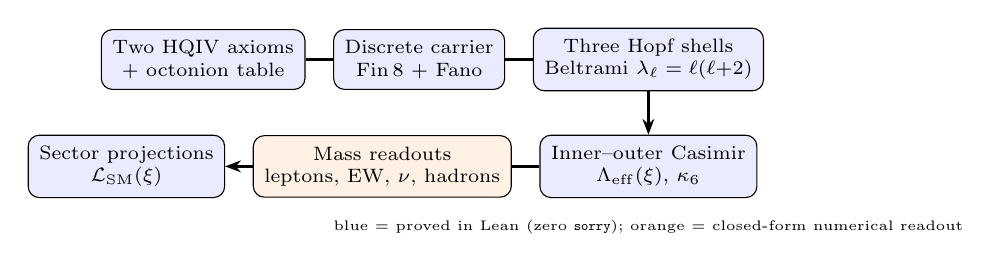
\begin{tikzpicture}[
    node distance=0.55cm and 0.35cm,
    box/.style={draw, rounded corners, align=center, inner sep=4pt, font=\scriptsize},
    proved/.style={box, fill=blue!8},
    readout/.style={box, fill=orange!10},
    arr/.style={-{Stealth[length=2mm]}, thick}
  ]
    \node[proved] (ax) {Two HQIV axioms\\+ octonion table};
    \node[proved, right=of ax] (car) {Discrete carrier\\$\mathrm{Fin}\,8$ + Fano};
    \node[proved, right=of car] (hopf) {Three Hopf shells\\Beltrami $\lambda_\ell=\ell(\ell{+}2)$};
    \node[proved, below=of hopf] (cas) {Inner--outer Casimir\\$\Lambda_{\mathrm{eff}}(\xi)$, $\kappa_6$};
    \node[readout, left=of cas] (mass) {Mass readouts\\leptons, EW, $\nu$, hadrons};
    \node[proved, left=of mass] (lsm) {Sector projections\\$\mathcal{L}_{\mathrm{SM}}(\xi)$};
    \draw[arr] (ax) -- (car) -- (hopf) -- (cas);
    \draw[arr] (cas) -- (mass) -- (lsm);
    \node[font=\tiny, below=0.15cm of cas] {blue = proved in Lean (zero \texttt{sorry}); orange = closed-form numerical readout};
  \end{tikzpicture}
  \caption{Constructive pipeline from axioms to the effective Standard Model Lagrangian at epoch $(\xi,\Phi,t)$.}
  \label{fig:pipeline}
\end{figure}

\begin{table}[ht]
  \centering
  \caption{Claim status at a glance.}
  \label{tab:claim-status}
  \footnotesize
  \begin{tabular}{>{\raggedright\arraybackslash}p{0.34\linewidth}>{\raggedright\arraybackslash}p{0.12\linewidth}>{\raggedright\arraybackslash}p{0.40\linewidth}}
    \toprule
    Claim & Status & Lean anchor \\
    \midrule
    Discrete Hopf shells + contact spectrum & Proved & \hyperref[lean:hopf-shell-complex]{Hopf shell complex} \\
    $\kappa_6=\eta_{\mathrm{local}}\,\gamma\,C_2$; $C_2=56/45$ at lock-in & Proved & \hyperref[lean:kappa6-bridge]{$\kappa_6$ mass bridge} \\
    O-Maxwell 1-jet Rindler law $1+(\gamma/2)m$ & Proved (scaffold) & \hyperref[lean:omaxwell-1jet]{O-Maxwell 1-jet} \\
    Five sector equalities of $\mathcal{L}_{\mathrm{SM}}$ & Proved & \hyperref[lean:sm-lagrangian-bridge]{SM Lagrangian bridge} \\
    Global hadron excitation readout & Closed-form readout & \hyperref[lean:global-hadron-readout]{Global hadron readout} \\
    Finite SM anomaly traces (one gen.\ $\times$3) & Proved & \hyperref[lean:anomaly-cancellation]{Anomaly cancellation} \\
    Patch instanton/$\theta$/Chern/winding discharge & Proved & \hyperref[lean:patch-topology]{Patch topology discharge} \\
    Strong-color $\mathfrak{su}(3)$ chart Lie law ($f^{abc}$) & Proved (optional cert) & \hyperref[lean:strong-color-su3]{Strong-color SU(3) chart} \\
    Weak $\mathfrak{su}(2)$ non-abelian kinematic chart & Proved & \hyperref[lean:weak-higgs-scaffold]{Weak/Higgs scaffold} \\
    CKM/PMNS from Fano cycle overlaps & Open (scaffold) & \hyperref[lean:t10-mixing-scaffold]{Generation mixing scaffold} \\
    Light-cone $\mathfrak{so}(8)$ holonomy discharge & Proved & \hyperref[lean:zeta-holonomy-discharge]{Sector zeta and holonomy discharge} \\
    Fibre-torsion subleading sector zeta & Proved & \hyperref[lean:zeta-holonomy-discharge]{Sector zeta and holonomy discharge} \\
    Shell-to-harmonic mode limit & Proved & \hyperref[lean:lightcone-qft-bridge]{Light-cone QFT bridge} \\
    Rapidity-phase Lorentz closure ($1{+}1$ boosts; $3{+}1$ embed) & Proved & \hyperref[lean:rapidity-lorentz-closure]{Rapidity--Lorentz closure} \\
    Spatial-rotation Lorentz closure ($O(3)$ readouts) & Proved & \hyperref[lean:spatial-rotation-lorentz-closure]{Spatial-rotation Lorentz closure} \\
    SO(8) four-edge Wilson plaquette holonomy & Proved (partial) & \hyperref[lean:so8-plaquette-holonomy]{SO(8) plaquette holonomy} \\
    Non-abelian holonomy + rotated-frame measure & Partial & \hyperref[lean:non-abelian-holonomy-measure]{Non-abelian holonomy measure} \\
    Abelian Wilson--kinetic plaquette equivalence & Proved & \hyperref[lean:action-holonomy-glue]{Action holonomy glue} \\
    Discrete action strong Poincaré invariance & Partial & \hyperref[lean:discrete-action-poincare]{Discrete action Poincaré scaffold} \\
    Nielsen external $C^\infty$ bundle / contact theorems & Not claimed & --- \\
    Continuum path-integral measure choice & Not claimed & --- \\
    \bottomrule
  \end{tabular}
\end{table}

\begin{scopebox}
\textbf{Proved} (zero \texttt{sorry}, two axioms + octonion tables): discrete Hopf shells; inner--outer Casimir mechanism and $\kappa_6$ factorisation; ground and excited readouts; five sector Lagrangian equalities; Yukawa linearity; total-action split.

\textbf{Discharged on the accessible patch:} explicit SM cubic and mixed anomaly-trace cancellation (\hyperref[lean:anomaly-cancellation]{Anomaly cancellation}); single-sector instanton, $\theta$, first-Chern, and $U(1)$ winding discharge (\hyperref[lean:patch-topology]{Patch topology discharge}); fibre-torsion subleading sector zeta and light-cone $\mathfrak{so}(8)$ holonomy on integrable Hopf shells, including abelian plaquette flatness and weak/colour non-abelian commutator certificates (\hyperref[lean:zeta-holonomy-discharge]{Sector zeta and holonomy discharge}, \hyperref[lean:action-holonomy-glue]{Action holonomy glue}, \hyperref[lean:weak-higgs-scaffold]{Weak/Higgs scaffold}); full four-edge SO(8) matrix Wilson plaquettes with pinned $(G_0,G_4)$ non-abelian witness (\hyperref[lean:so8-plaquette-holonomy]{SO(8) plaquette holonomy}); shell-to-harmonic mode limit (\hyperref[lean:lightcone-qft-bridge]{Light-cone QFT bridge}); rapidity-phase Lorentz closure on the null-lattice carrier with scalar $\phi$ and \texttt{zetaHQIVTerm} phase invariance (\hyperref[lean:rapidity-lorentz-closure]{Rapidity--Lorentz closure}); spatial $O(3)$ rotation invariance of flyby/CMB/fluid readouts (\hyperref[lean:spatial-rotation-lorentz-closure]{Spatial-rotation Lorentz closure}). Full detail: §\ref{sec:patch-continuum-bridge}.

\textbf{Partial / open on the patch:} Haar measure normalization on rotated charts (\hyperref[lean:non-abelian-holonomy-measure]{Non-abelian holonomy measure}); flat HQVM kinetic invariance under full \texttt{boostDiscretePotential41} and the embedded $(t,x^1)$ sub-target (\hyperref[lean:discrete-action-strong-poincare]{Discrete action strong Poincaré bridge}, bundled in \hyperref[lean:discrete-action-poincare]{Discrete action Poincaré scaffold}). \textbf{Discharged on the partial strong-Poincaré slice:} abelian Wilson--kinetic equivalence (\hyperref[lean:action-holonomy-glue]{Action holonomy glue}); fiber matrix Wilson + scalar-$\phi$ \texttt{action\_O\_Maxwell} rule (\hyperref[lean:discrete-action-strong-poincare]{Strong Poincaré bridge}).

\textbf{Not claimed:} Nielsen-style external smooth principal bundles, K\"ahler/contact self-adjointness, and path-integral measure choice on a \emph{separate} $C^\infty$ base---not because HQIV lacks anomaly cancellation, non-abelian holonomy, or sector zeta on the octonion light-cone carrier, but because those external classification theorems are not reproved as prerequisites. The patch net is the entire accessible universe, indexed by $\mathfrak{so}(8)$ on the light cone---a literal continuum rewrite would erase the discrete index carrying the predictions.

\textbf{Epoch choice:} laboratory PDG comparisons use $\xi_{\mathrm{lock}}=5$, $\Phi=t=0$. Cosmology uses the same $C_2(\xi)$ on the hot chart (\S\ref{sec:c2-rindler}). No per-flavour mass injection.

\textbf{Single scale witness (anti-fitting discipline):} exactly one dimensionful observable may anchor a given export or solve (\leanterm{scale witness discipline}{lean:scale-witness}{Hqiv/Physics/ScaleWitness.lean}). Default: proton at $\mathrm{referenceM}=4$. CODATA $1/\alpha$ \cite{codata2018}, $\eta_{\mathrm{obs}}$, and FIRAS $T_{\mathrm{CMB}}$ are \emph{predictions or comparison layers}, never simultaneous row inputs (\S\ref{subsec:scale-witness}).
\end{scopebox}

\begin{table}[ht]
  \centering
  \caption{Recurring symbols (horizon coordinate $\xi$, lapse parameters $\Phi,t$).}
  \label{tab:symbols}
  \small
  \begin{tabular}{p{0.22\linewidth}p{0.72\linewidth}}
    \toprule
    Symbol & Meaning \\
    \midrule
    $\xi$ & Horizon coordinate; $\xi=T_{\mathrm{Pl}}/T$ on the temperature ladder \\
    $\Phi$, $t$ & HQVM lapse/scalar slots in $C_2(\xi,\Phi,t)$ and observer detuning \\
    $\Lambda_{\mathrm{eff}}(\xi)$ & Inner--outer Casimir scale at $\xi$ \\
    $G(\xi)$ & Heavy-sector gap (relative Casimir scale); lepton ground anchor \\
    $M_n^{\mathrm{Hopf}}$ & Dimensionless Beltrami/sc sector-determinant body \\
    $m_n(\xi)$ & Charged-lepton mass triplet at $\xi$ \\
    $\Lambda_{\mathrm{Hopf}}(\xi)$ & $\sqrt{2\pi}\,v(\xi)\,\kappa_6$ spectral scale \\
    $\kappa_6$ & Topological suppression; $\kappa_6=\eta_{\mathrm{local}}\,\gamma\,C_2$ \\
    $\eta_{\mathrm{obs}}$ & Observed baryon-to-photon ratio $n_B/n_\gamma=6.10\times 10^{-10}$ \\
    $\eta_{\mathrm{local}}(\xi)$ & $\eta_{\mathrm{obs}}\,B_{\mathrm{curv}}(\xi)$; equals $\eta_{\mathrm{obs}}$ when $B_{\mathrm{curv}}=1$ \\
    $C_2$ & Second-order lapse concentration ($\delta$-dressed Rindler ratio; $56/45$ at lock-in) \\
    $v(\xi)$ & Dynamic electroweak vev at $\xi$ \\
    $t_{\mathrm{app}}$ & Look-back time: integrated null-geodesic span; observational age ($\approx 13.8\,\mathrm{Gyr}$) \\
    $t_{\mathrm{wall}}$ & Wall-clock proper time: $d\tau=N\,dt$ on the HQVM fundamental clock \\
    $\phi(m)$ & Auxiliary field $=2/T(m)=2(m+1)$; threads lapse, O-Maxwell, and Friedmann sectors \\
    $R_{\mathrm{in}}$ & Trapped-inside ratio on the meta-horizon shell \\
    $\omega K(\xi)$ & Normalised curvature primitive for Casimir running \\
    O-Maxwell & Maxwell's equations on octonions: eight-channel abelian gauge action on $\mathrm{Fin}\,8$ with phase-gradient source $J\cdot A$ \\
    \bottomrule
  \end{tabular}
\end{table}

\subsection{Patch QFT and the continuum readout layer}
\label{sec:patch-continuum-bridge}

Readers trained in continuum quantum field theory often ask three related questions: whether the HQIV patch is a UV regulator that must be sent to a smooth limit; whether anomaly cancellation, non-abelian holonomy, and path-integral measure are deferred to that limit; and what discrete upgrade would be required to match textbook gauge consistency. In HQIV the answers are already constructive and largely machine-checked.

\paragraph{The patch is not a mesh tile.}
The accessible patch is the \emph{entire causally accessible universe}: horizon-limited shell data, finite charts, and mode budgets on the octonion light-cone carrier. There is no observables layer outside this patch net waiting to be recovered by refinement. Familiar smooth-spacetime and $\mathcal{L}_{\mathrm{SM}}$ notation is therefore an \textbf{IR readout dictionary} for cross-citation with the standard literature, not a missing UV completion.

\paragraph{What ``projects to continuum QFT'' means.}
Three proved bridges connect patch data to continuum language without replacing the discrete ontology:
\begin{enumerate}[label=(\roman*),nosep]
\item \textbf{Sector projection.} The five equalities $S_{\mathrm{HQIV}}\Rightarrow\mathcal{L}_{\mathrm{SM}}$ (\hyperref[lean:sm-lagrangian-bridge]{SM Lagrangian bridge}) exhibit the textbook Lagrangian as an explicit projection of the discrete octonion action at epoch $(\xi,\Phi,t)$.
\item \textbf{Chart operators and holonomy.} Discrete Laplacian/Poisson stencils, plaquette transport, and cyclic O-Maxwell holonomy on the patch chart carry proved flatness and limit identities (\hyperref[lean:patch-qft-bridge]{Patch QFT bridge}, \hyperref[lean:action-holonomy-glue]{Action holonomy glue}, \hyperref[lean:readout-gauge-seed]{Readout gauge seed}).
\item \textbf{Controlled asymptotic mode content.} As shell index grows, the cumulative accessible mode budget divided by spherical-harmonic counting tends to a definite ratio---the emergent effective-mode law used in the horizon continuum package (\hyperref[lean:lightcone-qft-bridge]{Light-cone QFT bridge}). This is a proved shell$\to$harmonic limit on the same null ladder, not an unverified mesh-refinement conjecture.
\end{enumerate}

\paragraph{Gauge consistency discharged on the patch (proved).}
The obligations readers normally associate with continuum QFT are already finite statements on the carrier that produces the numerical readouts:
\begin{itemize}[nosep]
\item \textbf{Anomaly cancellation.} Explicit one-generation Standard-Model content yields vanishing $U(1)_Y^3$, grav--$U(1)_Y$, $SU(3)^2U(1)_Y$, $SU(2)^2U(1)_Y$, and $SU(3)^3$ trace coefficients; three generations are a finite label sum of the same cancelled block (\hyperref[lean:anomaly-cancellation]{Anomaly cancellation}, witness \leanid{sm_anomaly_free_three_generations}).
\item \textbf{Topological sector.} The patch abelian datum has a single sector: instanton, Pontryagin, first-Chern, and $U(1)$ winding charges vanish on patch data; the $\theta$ contribution is therefore $\theta$-independent (\hyperref[lean:patch-topology]{Patch topology discharge}).
\item \textbf{Non-abelian structure.} Light-cone $\mathfrak{so}(8)$ Lie closure; G$_2\cup\{\Delta\}$ chart; admissible holonomy on integrable Hopf shells; abelian cyclic plaquette flatness; proved $\mathfrak{su}(2)$ Pauli non-commutativity; optional global $\mathfrak{su}(3)$ Gell--Mann bracket law (\hyperref[lean:so8-closure]{SO(8) Lie closure}, \hyperref[lean:zeta-holonomy-discharge]{Sector zeta and holonomy discharge}, \hyperref[lean:weak-higgs-scaffold]{Weak/Higgs scaffold}, \hyperref[lean:strong-color-su3]{Strong-color SU(3) chart}).
\item \textbf{Sector zeta readout.} Leading Beltrami sector determinant matched to lattice amplitude at observer offset $\delta=0$, plus generation-indexed fibre-torsion subleading required for the charged-lepton band (\hyperref[lean:zeta-holonomy-discharge]{Sector zeta and holonomy discharge}, \hyperref[lean:global-detuning]{Global detuning}).
\item \textbf{Rapidity phase and Lorentz invariance.} \texttt{NullLatticeEvent} charts into $1{+}1$ Minkowski space by $\Lambda(\eta)(1,1)$; rapidity addition is boost-equivariant; \texttt{minkowskiInner11} and the embedded \texttt{minkowskiSq4} plane are invariant; \texttt{polarAngleFromRapidity} and the \texttt{zetaHQIVTerm} phase are unchanged under the Lorentz-scalar $\phi$ rule (\hyperref[lean:rapidity-lorentz-closure]{Rapidity--Lorentz closure}, witness \leanid{rapidity_lorentz_closure_discharged}).
\end{itemize}

\paragraph{What remains external (honest scope boundary).}
Lean does \emph{not} re-prove Nielsen's classification theorems on a \emph{separate} smooth principal-bundle or contact-manifold base, nor does it fix a textbook path-integral measure on that external $C^\infty$ carrier. Those statements are comparison-layer prerequisites in continuum TUFT, not load-bearing inputs here: the patch carrier already determines the anomaly traces, holonomy transport, topological charges, and sector zeta bodies used for mass and coupling readouts. Full CKM/PMNS unitary discharge from Fano cycle overlaps remains scaffold-only (\hyperref[lean:t10-mixing-scaffold]{Generation mixing scaffold}).

\paragraph{Module map (reproducibility).}
Table~\ref{tab:claim-status} and Appendix~\ref{app:lean-catalog} index the discharge bundles; the synthesis-specific upgrade lives in \hyperref[lean:zeta-holonomy-discharge]{Sector zeta and holonomy discharge}, with supporting algebra in \hyperref[lean:so8-closure]{SO(8) Lie closure}, topology in \hyperref[lean:hopf-shell-complex]{Hopf shell complex}, and continuum-bridge limits in \hyperref[lean:lightcone-qft-bridge]{Light-cone QFT bridge}.

\subsection{Background and reader contract}
\label{sec:background}

\noindent\textbf{Position in the publication chain.}
This is a Tier~2 synthesis paper in the HQIV series. Tier~0 fixes the framework
\cite{ettinger2026hqiv,hqiv-lightcone-paper,hqiv-so8-paper}; Tier~1 companions
\cite{hqiv-3d-growth-paper,hqiv-oct-action-paper,hqiv-kirchhoff-paper,hqiv-thermo-arrow-paper}
are on Zenodo.

\noindent\textbf{Nielsen TUFT and HQIV.}
Nielsen's TUFT provides the topological tool (complex Hopf fibration, Hopf-shell contact spectra, sector determinants) and the synthesis vision. This work realises those shells dynamically on the HQIV carrier, derives inner--outer Casimir balance from informational monogamy, and integrates the spectrum into $\mathcal{L}_{\mathrm{SM}}$ \cite{glashow1961,weinberg1967,salam1968,yang1954}. HQIV-specific signatures include longitudinal electromagnetic forces from the O-Maxwell phase-gradient term (absent from pure continuum TUFT) and exact rationals such as $C_2=56/45$ at lock-in.

\noindent\textbf{Standard Model and gauge-theory context.}
The textbook Lagrangian organizes non-Abelian gauge kinetic terms \cite{yang1954,tHooft1971,tHooft1972,gross1973,politzer1973,wilczek1973}, electroweak unification \cite{glashow1961,weinberg1967,salam1968,fermi1934}, scalar mass generation \cite{higgs1964,englert1964,nambu1960,goldstone1961}, and fermion Yukawa hierarchies \cite{yukawa1935,cabibbo1963,kobayashi1973,gellmann1964}; consolidated treatments appear in \cite{pdg2024,peskin1995,schwartz2014}. HQIV does not re-derive those structures from first principles: it exhibits a discrete octonion action whose sector projections match the same $\mathcal{L}_{\mathrm{SM}}$ once the TUFT/Hopf mass chart supplies the Yukawa weights.

\noindent\textbf{Patch-ontology contract.}
The accessible patch is the ontology; smooth-manifold textbook notation is an IR readout dictionary for cross-citation only. Anomaly cancellation, non-abelian holonomy on the light-cone $\mathfrak{so}(8)$ carrier, topological-sector discharge, and sector zeta subleading are \emph{proved} on that patch---not deferred to an uncontrolled continuum limit (§\ref{sec:patch-continuum-bridge}, Table~\ref{tab:claim-status}).

\subsection{The two HQIV axioms in one page}
\label{sec:two-axioms}

\paragraph{Axiom I (discrete light-cone combinatorics).}
New modes at shell index $m$ follow $N_{\mathrm{modes}}(m)=4(m+2)(m+1)$. The temperature ladder is $T(m)=1/(m+1)$; the auxiliary field $\phi(m)=2/T(m)=2(m+1)$. Truncation of the null lattice forces $\alpha=3/5$ at every order. \emph{Forbids:} importing a continuum limit or external coupling fits as definitions.

\paragraph{Axiom II (informational-energy monogamy).}
Horizon-area monogamy fixes the ADM lapse and HQVM metric; the overlap channel is $\gamma=2/5$. Localization energy $\Theta_{\mathrm{local}}^{-1}$ and the HQVM increment $N-1$ enter observer detuning (\S\ref{sec:c2-rindler}). \emph{Forbids:} injecting PDG masses \cite{pdg2024} or a fitted Yukawa matrix \cite{yukawa1935,cabibbo1963,kobayashi1973} as inputs to the proved bridge.

\paragraph{Derived layer.}
From the concrete octonion multiplication table \cite{baez2002octonions,Dixon1994,Gunaydin1974} one constructs the O-Maxwell action $S_O^{\mathrm{Maxwell}}(J,A,\phi)$---Maxwell's equations on octonions \cite{maxwell1865,jackson1999}---and its sector projections. Masses are \emph{readouts} of the Casimir chart at $(\xi,\Phi,t)$, not axioms \cite{casimir1948}.

\section{Hopf-Shell Structures on the Discrete Octonion Carrier}

Nielsen's TUFT establishes that the complex Hopf fibration \cite{hopf1931,Husemoller1994,Milnor1956,steenrod1951} is the natural topological setting for charge-quantised U(1) theories and that its nested shells ($S^1$, $S^3$, $S^5$, …) furnish the gauge factors of the Standard Model together with contact Beltrami spectra \cite{beltrami1892,Geiges2008} capable of generating the mass hierarchy from a single scale.

In the HQIV framework these Hopf shells arise dynamically on the discrete octonion carrier. From the light-cone axiom the octonion-indexed null lattice carries a Fano incidence geometry. The three dominant shell structures that emerge (corresponding to the weak, strong, and hypercharge channels under the triality decomposition of $\mathfrak{so}(8)$) are the discrete realisations of Nielsen's Hopf shells. They are not inserted by hand; they are the integrable three-shell complex supported by the carrier combinatorics already fixed by the first axiom.

On each of these discrete shells we have well-defined contact data whose eigenvalues follow the algebraic law $\lambda_\ell = \ell(\ell+2)$ familiar from the continuum $S^3$ Beltrami operator \cite{beltrami1892,RaySinger1971}, with multiplicities and winding sectors descending from discrete triality. The second (monogamy) axiom supplies the thermal response of these shells through the lapse and auxiliary field $\phi(m)$. The longitudinal electromagnetic forces generated by the phase-gradient term in the O-Maxwell action are native to this same carrier; they constitute an HQIV-specific signature (Figure~\ref{fig:hopf-compare}).

\begin{figure}[ht]
  \centering
  \footnotesize
  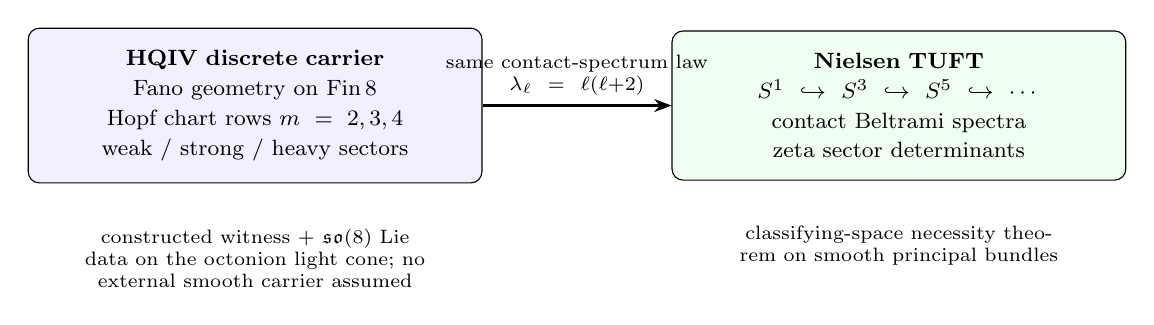
\begin{tikzpicture}[
    box/.style={draw, rounded corners, align=center, inner sep=8pt, text width=5.2cm, font=\footnotesize},
    arr/.style={-{Stealth[length=2.2mm]}, thick},
    lbl/.style={font=\scriptsize, align=center}
  ]
    \node[box, fill=blue!6] (disc) {\textbf{HQIV discrete carrier}\\[0.15em]
      Fano geometry on $\mathrm{Fin}\,8$\\[0.15em]
      Hopf chart rows $m=2,3,4$\\[0.15em]
      weak / strong / heavy sectors};
    \node[box, fill=green!6, right=2.4cm of disc] (cont) {\textbf{Nielsen TUFT}\\[0.15em]
      $S^1\hookrightarrow S^3\hookrightarrow S^5\hookrightarrow\cdots$\\[0.15em]
      contact Beltrami spectra\\[0.15em]
      zeta sector determinants};
    \draw[arr] (disc) -- node[above, lbl, text width=3.4cm] {same contact-spectrum law\\$\lambda_\ell=\ell(\ell{+}2)$} (cont);
    \node[below=0.45cm of disc, lbl, text width=5.2cm] {constructed witness + $\mathfrak{so}(8)$ Lie data on the octonion light cone; no external smooth carrier assumed};
    \node[below=0.45cm of cont, lbl, text width=5.2cm] {classifying-space necessity theorem on smooth principal bundles};
  \end{tikzpicture}
  \caption{Discrete Hopf-shell chart on the octonion carrier (left) and Nielsen's nested Hopf fibration (right) carry the same contact-spectrum law; methodology differs (witness vs classification).}
  \label{fig:hopf-compare}
\end{figure}

\section{Complementary Perspectives}

Nielsen's Topological Unified Field Theory stands as a striking achievement. Starting from the classification theorem for principal U(1)-bundles \cite{Milnor1956,Milnor1956b,MilnorStasheff1974,steenrod1951} and the two minimal axioms of charge quantisation and completeness, she proves that any unified gauge theory satisfying these conditions must realise its U(1) sector on the universal complex Hopf fibration and its finite approximations. The nested shells then force the Standard-Model gauge factors as canonical reductions, while the Kähler geometry of the base together with fibre torsion supplies a gravitational sector of Einstein--Cartan type. On each shell the generalised Beltrami operator acting on the contact distribution is elliptic and essentially self-adjoint; its zeta-regularised spectral determinants \cite{minakshisundaram1949,RaySinger1971,Cheeger1979,Muller1978,witten1979}, together with the intersection theory of admissible cycles, generate the entire mass and coupling hierarchy once a single empirical scale is supplied.

The discrete octonion-carrier framework developed in the HQIV series reaches closely related geometric structures from a different point of departure. Rather than beginning with the classification of bundles, it begins with a discrete null-lattice metric whose combinatorial rules are fixed by horizon-area monogamy on a finite octonion-indexed carrier. In this ontology the U(1) sector itself emerges from the light-cone geometry and the sectorial projection of the discrete octonion action. The three-shell Hopf data, admissible cycles, and contact torsion matrices appear as explicitly constructed, machine-verified witnesses of the same topological objects Nielsen derives, but now realised on a finite carrier without any appeal to a continuum limit or to the classification theorem as a starting axiom.

The two programmes therefore differ both methodologically and in the phenomenological questions they naturally address. Nielsen's construction collapses standard differential-geometric structures onto the Hopf geometry, yielding powerful statements of necessity and a unified account of mass generation from spectral geometry. The discrete construction, by contrast, derives its gauge structure and its temperature ladder from the same null-lattice combinatorics; as a result it takes the identification of a consistent reference epoch on the physical-temperature ladder as its primary phenomenological input. This choice makes cosmological evolution directly accessible and yields predictions such as temperature-dependent spectra, birefringence evolution, and longitudinal force signatures that follow without additional postulates.

A further structural difference appears in the electromagnetic sector. The O-Maxwell formulation on the octonion carrier yields a longitudinal force component generated by the phase-gradient term. No counterpart to this longitudinal channel arises in the topological construction, which recovers the standard transverse Maxwell structure on the fundamental Hopf fibre \cite{maxwell1865,jackson1999}.

What remains most striking is the depth of convergence. Both frameworks identify the nested Hopf shells, the contact Beltrami spectra, and the necessity of a single reference scale as the origin of the observed mass hierarchy. Nielsen's analysis demonstrates why such a structure is topologically forced; the discrete realisation exhibits how it can be rendered finite, formally verifiable, and dynamically responsive to the thermal history of the universe. The two routes are therefore complementary rather than competitive.

\subsection{Formal verification: Lean as a TUFT reproduction and its limits}
\label{sec:lean-tuft-reproduction}

The public HQIV Lean library (\url{https://github.com/HQIV/hqiv-lean}) is, in most load-bearing respects, a \emph{formal-methods reproduction} of Nielsen's TUFT synthesis on a finite discrete carrier. The honest geometry is already \emph{continuous Lie data on the octonion light-cone carrier}: a proved $\mathfrak{so}(8)$ Lie algebra (28 antisymmetric generators, bracket closure), the G$_2\cup\{\Delta\}$ chart with preferred $(e_1,e_7)$ U(1) plane, and hopf-shell torsion matrices supplying admissible holonomy on integrable shells. Lean does not re-prove Nielsen's \emph{external} continuum classification theorems (principal U(1)-bundle completeness on a separate smooth base, Kähler-base geometry, elliptic self-adjointness on smooth contact manifolds). Instead, it constructs explicit witnesses of the same topological objects---three integrable Hopf shells, contact Beltrami eigenvalues $\lambda_\ell=\ell(\ell+2)$, sector zeta-determinant bodies, admissible-cycle holonomy rows, outer neutral-shell suppression, and trapped-inside excitation ratios---and machine-checks the arithmetic identities that turn those witnesses into mass readouts once a reference epoch is chosen. Python evaluation scripts mirror the same closed forms for PDG comparison tables (Appendix~\ref{app:lean-catalog}); they are regression layers, not independent fits.

\paragraph{What Lean formally reproduces from TUFT.}
\begin{itemize}[nosep]
\item \textbf{Hopf-shell chart.} Weak, strong, and heavy Beltrami rows ($m=n+1$ on winding sectors $n=1,2,3$) with the same contact spectrum law as Nielsen's Sector Determinant Lemma.
\item \textbf{Charged leptons.} Full sector-determinant readout: leading Beltrami body $M_n^{\mathrm{Hopf}}$ plus generation-indexed fibre-torsion subleading from the Ray--Singer $S^3$ residue (\S\ref{sec:reader-guide}, Table~\ref{tab:pdg-lockin}).
\item \textbf{Neutrinos.} Outer neutral Hopf shell, holonomy ratios $(48,96,144)/91$, and generation-mixing steepening on the outer sector---Nielsen's outer-shell programme without a seesaw.
\item \textbf{Electroweak closure.} Outer-horizon SU(2) and scalar witnesses with lock-in vev bridge; geometric $\sin^2\theta_W$ from electroweak vs EM Gauss-shell detuning.\leanfnterm{Electroweak boson readout}{lean:ew-boson-readout}{Hqiv/Physics/TuftElectroweakBosonReadout.lean}
\item \textbf{Hadronic excitations.} Global trapped-inside law with valence content weights, split inversion, and parity-dependent excitation coupling---one functional form for baryons and mesons (Definition~\ref{def:global-mass}).
\item \textbf{Single-scale vision.} One electroweak reference fixes the hierarchy; HQIV makes that scale the output of inner--outer Casimir balance at $(\xi,\Phi,t)$.
\end{itemize}

\paragraph{Where the Lean development diverges from continuum TUFT.}
\begin{itemize}[nosep]
\item \textbf{Starting axioms.} HQIV begins from discrete light-cone combinatorics and informational monogamy on an octonion-indexed null lattice, not from Nielsen's bundle-classification axioms. The Hopf shells are \emph{constructed and proved} on the carrier rather than inferred as the unique U(1) classifying geometry.
\item \textbf{Light-cone $\mathfrak{so}(8)$ vs external smooth carrier.} HQIV carries proved continuum Lie algebra data on the octonion light-cone geometry---not an external smooth contact manifold glued on afterward. Load-bearing equalities remain patch-indexed witnesses on $\mathrm{Fin}\,8$ (and related finite index sets); smooth $\mathcal{L}_{\rm SM}$ notation and Nielsen's separate $C^\infty$ bundle theorems are cross-citation / comparison layers (patch-ontology contract in the abstract).
\item \textbf{Temperature dynamics.} The effective vev $v(\xi)$, heavy gap $G(\xi)$, and $\kappa_6(\xi,\Phi,t)$ are explicit functions of cosmic temperature. Pure continuum TUFT fixes spectral geometry at one scale; HQIV propagates the entire Lagrangian with epoch.
\item \textbf{HQIV-specific physics.} Longitudinal electromagnetic forces from the O-Maxwell phase-gradient term have no TUFT counterpart. Exact discrete rationals ($\alpha=3/5$, $\gamma=2/5$, $C_2=56/45$ at lock-in) are axiom-fixed, not emergent reals from smooth spectral analysis.
\item \textbf{Shell ontology.} HQIV \texttt{referenceM} (substrate export pin for cosmology and proton convention) and TUFT \texttt{tuftHeavyChartShell} ($m=n+1$ on the heavy Hopf winding) are \emph{different names}; Lean proves numeric coincidence under current pins, not chart identification (see \hyperref[lean:shell-chart]{TUFT shell chart} in Appendix~\ref{app:lean-catalog} and Appendix~\ref{app:shell-ontology}).
\item \textbf{Electroweak mixing implementation.} The $Z$ mass uses geometric shell detuning rather than the naive $(g_{\mathrm{SU2}}+g_{\mathrm{U1}})$ line (retained as a diagnostic overshoot). The primary $W$ readout is factorised as closure $\times$ vev bridge $\times$ heavy-gap scale; the equivalent geometric-mean form is proved equal for arbitrary lock-in vev (\texttt{tuftMW\_geometricMean\_atXi\_GeV\_eq}).
\item \textbf{Scope boundaries.} Lean certifies the structural bridge, full patch gauge-consistency discharge, and readout arithmetic with zero \texttt{sorry} (§\ref{sec:patch-continuum-bridge}, \S\ref{subsec:patch-gauge-consistency}, Table~\ref{tab:claim-status}). It does \emph{not} claim Nielsen's external smooth principal-bundle / contact-manifold theorems or path-integral measure choice on a separate $C^\infty$ carrier; CKM/PMNS unitary discharge remains scaffold-only.
\end{itemize}

\paragraph{Diagnostic layers (superseded TUFT/HQIV paths).}
Several older readout channels remain in the repository for regression only: legacy lepton shell quotients ($\sim 10^2$--$10^3\times$ PDG), meta-horizon operational catalog ($\sim 6$--$15\%$ overshoots), lepton-seeded dynamic towers ($\sim 2$--$3\times$ on hadrons), naive $Z$ and raw scalar-closure $H$ rows (Table~\ref{tab:legacy-hadron}, Table~\ref{tab:ew-bosons}). These are \emph{not} part of the primary TUFT reproduction; they document failed intermediate hypotheses on the way to the closed readouts above.

\paragraph{Reader contract.}
Treat Nielsen's TUFT as the topological synthesis programme and the Lean development as its discrete, epoch-aware, machine-checked realisation. Agreement with PDG \cite{pdg2024} at lock-in validates the witness arithmetic, not a point-by-point identity with every continuum intermediate step in Nielsen's manuscript. Disagreement would falsify the discrete witness chain or the epoch choice, not the Hopf-fibration classification theorem in the smooth category \cite{hopf1931,Milnor1956,steenrod1951}.

\subsection{Symbols and reader guide}
\label{sec:reader-guide}

\paragraph{Audience.}
The main text is addressed to readers of particle physics and mathematical physics who may know the Standard Model \cite{pdg2024,peskin1995,schwartz2014} and compact-manifold spectral theory \cite{RaySinger1971,Geiges2008} but who need not know the HQIV Lean codebase. Nielsen's TUFT programme \cite{NielsenTUFT2026} supplies the \emph{synthesis}: nested Hopf shells on the complex Hopf fibration, contact Beltrami operators, admissible-cycle holonomy, and sector zeta determinants that fix mass rungs from one electroweak reference. HQIV supplies the \emph{dynamic carrier}: a discrete octonion null lattice, inner--outer Casimir balance versus cosmic temperature, and machine-checked readouts at a chosen reference epoch.

\paragraph{What we borrow from Nielsen (TUFT).}
\begin{itemize}[nosep]
\item Nested shells $S^1\to S^{2n+1}\to\mathbb{C}P^n$ as the canonical U(1) classifying geometry.
\item Contact Beltrami spectra $\lambda_\ell=\ell(\ell+2)$ and zeta-regularized \emph{sector determinants} on each shell (Nielsen's Sector Determinant Lemma).
\item Admissible-cycle intersection data and holonomy rows that split generation rungs.
\item A single-scale vision: one reference fixes the hierarchy; HQIV makes that scale an explicit function of temperature.
\end{itemize}

\paragraph{Symbols and notation.}
Table~\ref{tab:symbols} lists recurring symbols. Nielsen's TUFT programme \cite{NielsenTUFT2026} supplies nested Hopf shells, contact Beltrami operators, admissible-cycle holonomy, and sector zeta determinants; HQIV supplies the dynamic null-lattice carrier, inner--outer Casimir balance, and machine-checked readouts at $(\xi,\Phi,t)$.

\section{The Dynamic Inner--Outer Casimir Mechanism}

Nielsen's TUFT supplies the topological vision of a single electroweak-scale reference generating the entire mass hierarchy through the spectral geometry of the Hopf shells. The key technical step that converts this vision into a fully dynamic, temperature-dependent spectrum is the inner--outer Casimir construction on the three-shell Hopf carrier realized on the discrete octonion carrier, together with its outer neutral singlet extension.

On the inner contact surfaces of the three integrable Hopf shells, the trapping selection functional (modulated by the continuous curvature primitive $\omega K(\xi)$ already present in the HQIV geometry) generates a geometric factor responsible for binding and for the heavy stabilisation gap \cite{casimir1948}. On the outer surface of the same carrier, the neutral singlet extension produces a suppression factor recovered as the coarse-grained readout of the outer fluctuation mode count. The effective scale at any horizon coordinate $\xi$ is therefore the ratio
\[
\Lambda_{\rm eff}(\xi) = \frac{\text{inner trapping}(\omega K(\xi))}{\text{outer suppression}}.
\]
Figure~\ref{fig:casimir-balance} summarises the flow; because $\omega K(\xi)$ is obtained by normalising the curvature primitive (logarithmic plus quadratic-logarithmic) against its value at the reference epoch, the scale becomes an explicit function of cosmic temperature once the physical-temperature--$\xi$ conversion supplied by the HQIV auxiliary field ladder is used.

\begin{figure}[ht]
  \centering
  \small
  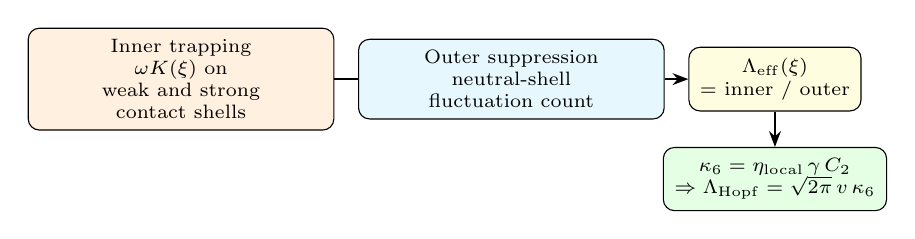
\begin{tikzpicture}[
    node distance=0.45cm and 0.3cm,
    box/.style={draw, rounded corners, align=center, inner sep=4pt, font=\scriptsize},
    arr/.style={-{Stealth[length=2mm]}, thick}
  ]
    \node[box, fill=orange!12, text width=3.6cm] (in) {Inner trapping\\$\omega K(\xi)$ on\\weak and strong\\contact shells};
    \node[box, fill=cyan!10, right=of in, text width=3.6cm] (out) {Outer suppression\\neutral-shell\\fluctuation count};
    \node[box, fill=yellow!12, right=of out] (ratio) {$\Lambda_{\mathrm{eff}}(\xi)$\\$=$ inner / outer};
    \node[box, fill=green!10, below=of ratio] (k6) {$\kappa_6=\eta_{\mathrm{local}}\,\gamma\,C_2$\\$\Rightarrow\Lambda_{\mathrm{Hopf}}=\sqrt{2\pi}\,v\,\kappa_6$};
    \draw[arr] (in) -- (out) -- (ratio);
    \draw[arr] (ratio) -- (k6);
  \end{tikzpicture}
  \caption{Inner--outer Casimir balance: trapping on contact shells versus outer neutral suppression sets the epoch-dependent scale fed into lepton, electroweak, and hadron readouts.}
  \label{fig:casimir-balance}
\end{figure}

The resulting lepton mass spectrum at any physical temperature is obtained in two steps. First the composite data on the carrier (zeta leading term on the heavy shell, torsion coefficient $4/5$, admissible holonomy row, chart factor $\xi/5$) supplies the instantaneous dynamic scale and hence the effective vacuum expectation value at that horizon coordinate. Then the Hopf spectral scale $\Lambda_{\rm Hopf}=\sqrt{2\pi}\,v(\xi)\,\kappa_6$ converts dimensionless Beltrami scalars into particle masses. Relative rungs within a sector are dimensionless; the \emph{absolute} MeV/GeV chart is fixed by one active scale witness (\S\ref{subsec:scale-witness}). Under the default proton lock-in, that witness is the locally measured proton mass at $\mathrm{referenceM}=4$; the electroweak vev is then an \emph{output} of the same Casimir chart, not an independent fit parameter.

This construction realises, in a discrete and formally verified setting, the single-scale derivation programme motivated by Nielsen's topology of the complex Hopf fibration, while simultaneously supplying the temperature dependence that any realistic cosmological model requires. Operational particle masses are downstream readouts of the chain $T\leftrightarrow \xi\leftrightarrow v\leftrightarrow m$; PDG masses \cite{pdg2024} enter only as comparisons of the readout.

The dimensionless topological suppression slot factorises as
\[
\kappa_6(\xi,\Phi,t)=\eta_{\mathrm{local}}(\xi)\,\gamma\,C_2(\xi,\Phi,t),
\]
where $\eta_{\mathrm{local}}(\xi)$ is the matter-fraction slot in the electroweak chart (introduced in §\ref{subsec:sm-inputs}), $\gamma=2/5$ is the monogamy overlap channel fixed by the second HQIV axiom, and $C_2$ is the explicit second-order Hopf/contact correction arising from the discrete lapse concentration (proved $C_2=56/45$ at lock-in with $\Phi=t=0$ in the Lean development). All three factors are explicit, parameter-free functions of the chosen now-slice; under proton lock-in, $\eta_{\mathrm{obs}}$ is a \emph{predicted} baryon-to-photon surplus (cross-check against Planck/CODATA \cite{planck2018cosmo,codata2018,coc2015}), not a second anchor in the same solve. The Rindler denominator law, the $\delta$-shift, the lock-in arithmetic, the legacy comparison, and off-lock-in running are developed in \S\ref{sec:c2-rindler}.

\subsection{Rindler ladder, \texorpdfstring{$\delta$-shift}{delta-shift}, and lapse concentration \texorpdfstring{$C_2$}{C2}}
\label{sec:c2-rindler}

\paragraph{Status: proved 1-jet chain; full spectral emergence open.}
The closed form $\texttt{detunedShellSurface}(m)=S(m)/\bigl(1+\tfrac{\gamma}{2}m\bigr)$ with $S(m)=(m+1)(m+2)$ is no longer a standalone postulate in the Lean development. A machine-checked chain (\hyperref[lean:omaxwell-1jet]{O-Maxwell 1-jet projection}, \hyperref[lean:fano-omaxwell-spectrum]{Fano O-Maxwell spectrum}) identifies the \textbf{1-jet Rindler factor} with a linearized projection of the eight-channel O-Maxwell action onto a canonical Fano incidence line:
\begin{enumerate}[label=(\roman*),nosep]
\item The parent generator ladder and phase-lift coefficient $\varphi(m)=2(m+1)$ supply a shell increment of projected mode strength $\Delta\mathrm{strength}=(1/3)\,m$ on any Fano line (normalization fixed by triality/Fano trace bookkeeping).
\item Linearizing the projected $\Delta$-coupled sector energy yields the action 1-jet $1+(3\gamma/2)\,\Delta\mathrm{strength}$.
\item Substituting $\Delta\mathrm{strength}=(1/3)m$ collapses the coefficient: $(3\gamma/2)\cdot(1/3)=\gamma/2$. Hence
\begin{align}
  \texttt{spectralFanoRindler1Jet}(L,m) &= 1 + \frac{\gamma}{2}\,m, \\
  \texttt{detunedShellSurface}(m) &= \frac{S(m)}{\texttt{spectralFanoRindler1Jet}(L,m)}.
\end{align}
\end{enumerate}
Higher jets (\texttt{rindlerDetuningThreeJet} with lock-in-centered curvature corrections) remain diagnostic; the load-bearing mass ratios use the \textbf{first jet} only. The remaining open step---replacing the affine scaffold by a full mode-selection/eigen-shell limit of the coupled O-Maxwell + $\varphi$ dynamics---is documented in the repository design note on modal-frequency emergence; the present paper treats the 1-jet law as \textbf{proved relative to the spectral projection definitions}, not yet as a uniqueness theorem for all continuum limits.

\begin{proofsketch}
Projected strength on a Fano line increments as $\Delta\mathrm{strength}=(1/3)m$ because $\varphi(m)=2(m+1)$ and spectral normalization is unity.
The action 1-jet is $1+(3\gamma/2)\Delta\mathrm{strength}$; substituting $(3\gamma/2)(m/3)=\gamma m/2$ yields $1+(\gamma/2)m$.
Identification with \texttt{detunedShellSurface} is one line of \texttt{simp} + \texttt{ring} per shell index.
\end{proofsketch}
\footnote{Lean witnesses \leanid{omaxwellProjectedStrengthIncrement_eq_one_third_shell}, \leanid{omaxwellActionDetuning1Jet_eq_rindler} in \hyperref[lean:omaxwell-1jet]{O-Maxwell 1-jet projection} (Appendix~\ref{app:lean-catalog}).}

\paragraph{Physical origin of the $\delta$-shift.}
The global detuning module packages a \textbf{scalar observer offset} $\delta$ in the denominator correction
$\texttt{rindlerDenWithDelta}(\delta,m)=1+\tfrac{\gamma}{2}m+\delta$.
The lapse-concentration factor $C_2$ compares the $\delta$-dressed denominator on the heavy TUFT chart row $m=4$ to the baseline Rindler ladder:
\begin{equation}
\label{eq:C2-lapse}
C_2(\xi,\Phi,t)
= \frac{1+\gamma}{2}\,
\frac{\texttt{rindlerDenWithDelta}\bigl(c_{\mathrm{rindler}}\,\mathrm{obs}(\xi,\Phi,t),\,m_{\mathrm{heavy}}\bigr)}
     {\texttt{rindlerDetuningShared}(m_{\mathrm{heavy}})},
\end{equation}
with $c_{\mathrm{rindler}}=\gamma/2$ and
\begin{equation}
\label{eq:obs-lapse}
\mathrm{obs}(\xi,\Phi,t)
= \Theta_{\mathrm{local}}(\xi)\,(1+\gamma) + \bigl(N(\Phi,\varphi(\xi),t)-1\bigr),
\qquad
\Theta_{\mathrm{local}}(\xi)=\xi/T_{\mathrm{Pl}}.
\end{equation}
Three ingredients motivate the \textbf{linear} entry of $\delta=c_{\mathrm{rindler}}\,\mathrm{obs}$ rather than an arbitrary function of the observer datum:
\begin{itemize}[nosep]
\item \textbf{Monogamy overlap.} The second HQIV axiom fixes $\gamma=2/5$ as the horizon overlap channel; the Rindler slope $c_{\mathrm{rindler}}=\gamma/2$ is the same coefficient already proved in the \leanterm{1-jet detuning law}{lean:detuning-law}{Hqiv/Physics/FanoDetuningFirstOrder.lean}. Using a different prefactor on $\mathrm{obs}$ would break the identification between first- and second-order detuning on the same chart.
\item \textbf{Informational localization.} $\Theta_{\mathrm{local}}^{-1}$ is the minimal localization energy slot on the temperature ladder. At lock-in with HQVM lapse unity ($\Phi=t=0$), $\mathrm{obs}=\xi(1+\gamma)$: the observer sits at finite horizon coordinate on the temperature ladder, so the shell denominator acquires a \textbf{first-order} correction proportional to localization, not a re-fit of the entire surface law.
\item \textbf{Phase-gradient / longitudinal channel.} The O-Maxwell action's phase-gradient coupling is the carrier-native way an observer datum enters the effective gauge potential. The HQVM lapse increment $N-1$ in \eqref{eq:obs-lapse} is the same scalar combination used in \hyperref[lean:global-detuning]{global detuning} hypotheses; $C_2$ is therefore the \textbf{lapse-concentration readout} of that datum on the heavy Hopf shell, not an independent Yukawa knob.
\end{itemize}

\paragraph{Lock-in value $C_2=56/45$.}
At $\xi_{\mathrm{lock}}=5$, $\Phi=t=0$, $m_{\mathrm{heavy}}=4$, $\gamma=2/5$, $T_{\mathrm{Pl}}=1$:
$\mathrm{obs}=7$, $\delta=7/5$, baseline denominator $9/5$, shifted denominator $16/5$, overlap factor $(1+\gamma)/2=7/10$, hence
\[
  C_2 = \frac{7}{10}\cdot\frac{16/5}{9/5}=\frac{112}{90}=\frac{56}{45}\approx 1.244.
\]
Lean: \texttt{tuftLapseConcentrationAtXi\_lockin\_zero} (\texttt{HopfShellBeltramiMassBridge.lean}).

\paragraph{Derived vs legacy $C_2$ (no re-fit).}
Before closure, the second-order slot was a regression constant $C_2^{\mathrm{legacy}}\approx 1.135$ retained only as \texttt{tuftHopfKappa6SecondOrderCorrectionLegacy}. The derived value is \textbf{$9.6\%$ higher}. Because $\kappa_6\propto C_2$ and $\Lambda_{\mathrm{Hopf}}\propto\kappa_6$, the shift would lower $\mu$ and $e$ by the same factor if nothing else moved; the $\tau$ anchor is fixed by the vev--$\kappa_6$ heavy scale. Table~\ref{tab:c2-legacy} shows that the framework \textbf{absorbed} the change: derived $C_2$ lands the lighter charged leptons \emph{closer} to PDG, while a hypothetical return to the legacy slot would undershoot by $\sim 9\%$. No other sector constant was retuned when $C_2$ was derived.

\begin{table}[ht]
  \centering
  \caption{$C_2$ closure: derived vs legacy second-order slot at $\xi_{\mathrm{ref}}=5$.}
  \label{tab:c2-legacy}
  \small
  \begin{tabular}{lrrr}
    \toprule
    Quantity & Derived & Legacy & Comment \\
    \midrule
    $C_2$ & $56/45\approx 1.244$ & $1.135$ & $+9.6\%$; proved, not fitted \\
    \diagnosticrow
    $\mu$ model / PDG & $0.999$ & $\approx 0.912$ & legacy would undershoot \\
    \diagnosticrow
    $e$ model / PDG & $0.998$ & $\approx 0.910$ & same factor ($\kappa_6$ linear) \\
    $\tau$ model / PDG & $1.000$ & $1.000$ & vev--$\kappa_6$ anchor unchanged \\
    \bottomrule
  \end{tabular}
\end{table}

\paragraph{Off-lock-in running (predictive content).}
With $\Phi=t=0$, \eqref{eq:C2-lapse}--\eqref{eq:obs-lapse} collapse to the closed form
\[
  C_2(\xi)=\frac{7}{10}\left(1+\frac{7\xi}{45}\right),
\]
monotone in the horizon coordinate: colder slices (larger $\xi$) concentrate lapse on the heavy chart; hotter slices suppress $C_2$ below unity. Table~\ref{tab:c2-xi} and Figure~\ref{fig:c2-xi} list and plot representative epochs on the $\xi$ ladder (reproducible from \scriptfile{hqiv_lean_physics_primitives.py}).

\begin{table}[ht]
  \centering
  \caption{Lapse concentration $C_2(\xi)$ at $\Phi=t=0$ (no free parameters).}
  \label{tab:c2-xi}
  \small
  \begin{tabular}{lrr}
    \toprule
    Horizon coordinate $\xi$ & $C_2(\xi)$ & $\kappa_6/\kappa_6(\xi_{\mathrm{lock}})$ \\
    \midrule
    $0.5$ & $0.754$ & $0.606$ \\
    $1$ & $0.809$ & $0.650$ \\
    $2$ & $0.918$ & $0.738$ \\
    $3$ & $1.027$ & $0.825$ \\
    $5$ (lock-in) & $1.244$ & $1.000$ \\
    $10$ & $1.789$ & $1.438$ \\
    \bottomrule
  \end{tabular}
\end{table}

\begin{figure}[ht]
  \centering
  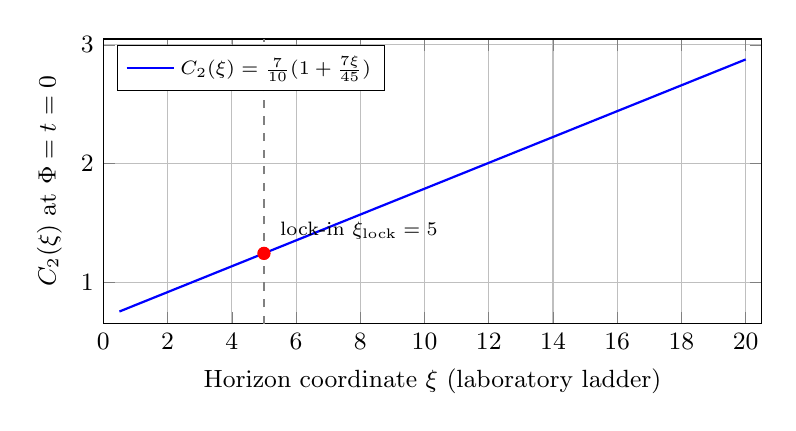
\begin{tikzpicture}
    \begin{axis}[
      width=0.82\textwidth,
      height=5.2cm,
      xmin=0, xmax=20.5,
      ymin=0.65, ymax=3.05,
      xlabel={Horizon coordinate $\xi$ (laboratory ladder)},
      ylabel={$C_2(\xi)$ at $\Phi=t=0$},
      grid=major,
      legend style={at={(0.02,0.98)},anchor=north west,font=\scriptsize},
      tick label style={font=\small},
      label style={font=\small}
    ]
      \addplot[thick, blue, domain=0.5:20, samples=80]
        {(7/10)*(1 + (7/45)*x)};
      \addplot[only marks, mark=*, mark size=2.2pt, red]
        coordinates {(5,1.244)};
      \draw[dashed, gray] (axis cs:5,0.65) -- (axis cs:5,3.05);
      \node[font=\scriptsize, anchor=south west] at (axis cs:5.2,1.28)
        {lock-in $\xi_{\mathrm{lock}}=5$};
      \legend{$C_2(\xi)=\tfrac{7}{10}(1+\tfrac{7\xi}{45})$}
    \end{axis}
  \end{tikzpicture}
  \caption{Lapse concentration $C_2(\xi)$ on the homogeneous chart at $\Phi=t=0$. Laboratory mass tables use the lock-in slice; BBN and cosmology probe other $\xi$ via dynamic opportunity weighting on the MeV temperature chart (\S\ref{sec:c2-rindler}).}
  \label{fig:c2-xi}
\end{figure}

On the BBN temperature chart the same $C_2(\xi)$ enters $\kappa_6=\eta_{\mathrm{obs}}\,B_{\mathrm{curv}}(\xi)\,\gamma\,C_2(\xi)$ with \textbf{dynamic opportunity weighting} rather than a lock-in mass re-fit: for $T\le T_{\mathrm{bn}}(\eta)$ the shell reaction clock multiplies by $(\kappa_{6,\mathrm{ref}}/\kappa_6)^{w_{C_2}(T)}$ with $w_{C_2}$ tied to the deuteron bottleneck.\footnote{Lean: \hyperref[lean:dynamic-bbn]{dynamic BBN baryogenesis}; script: \scriptfile{hqiv_dynamic_bulk_bbn.py}.}

\paragraph{Cosmological consistency check.}
The \emph{same} $C_2(\xi)$ slot that fixes laboratory $\kappa_6$ at $\xi_{\mathrm{lock}}$ enters the BBN integrator without extra MeV cutoffs. At $\eta_{10}\approx 6.2$ the dynamic-$C_2$ network yields $Y_p\approx 0.245$ and $D/H\approx 2.4\times 10^{-5}$ (audit: \path{data/integrator\_lean\_audit.json}), supporting the interpretation of $C_2$ as physical lapse running rather than a lock-in-only fit. Laboratory mass tables remain at $\xi_{\mathrm{ref}}=5$; cosmology probes $\xi(T)$ directly.

\subsection{Error budget and sensitivity}
\label{sec:error-budget}

The PDG ratios quoted in the executive summary are not fine-tuned to individual particles; they follow from closed forms at $\xi_{\mathrm{lock}}=5$ and are compared against the Particle Data Group compilation \cite{pdg2024}. Three independent sensitivity checks quantify how tight those matches are:

\paragraph{Lock-in coordinate $\xi$.}
A $\pm 1\%$ shift in $\xi_{\mathrm{lock}}$ moves $\mu/\mathrm{PDG}$ and $e/\mathrm{PDG}$ by $\approx\mp 0.5\%$ (via the vev--gap chart); $\pm 5\%$ in $\xi$ yields $\approx\mp 2\%$ on the lighter charged leptons while $\tau$ remains anchored. A $\gtrsim 5\%$ systematic mismatch across $\mu$ and $e$ at fixed $\xi$ would therefore indicate failure of the Casimir chart, not a per-flavour adjustment.

\paragraph{Subleading zeta terms.}
Dropping the fibre-torsion subleading (leading Beltrami body only) overshoots $\mu$ and $e$ by $\sim 1.5\%$--$1.8\%$ (Table~\ref{tab:pdg-lockin}, diagnostic rows). Including the generation-indexed subleading is required for the quoted $0.2\%$ lepton band.

\paragraph{$C_2$ closure vs legacy regression.}
Replacing derived $C_2=56/45$ with the pre-closure regression $C_2^{\mathrm{legacy}}\approx 1.135$ ($-9.6\%$ in $\kappa_6$) would lower $\mu$ and $e$ to $\sim 91\%$ of PDG with no change to other sector constants (Table~\ref{tab:c2-legacy}). The derived value improves the lighter-lepton matches while leaving $\tau$ exact.

The resulting masses are
\[
m_n(\xi)=\Lambda_{\rm Hopf}(\xi)\cdot M_n(\xi),
\]
where $\Lambda_{\rm Hopf}(\xi)=\sqrt{2\pi}\,v(\xi)\,\kappa_6(\xi,\Phi,t)$ and the dimensionless $M_n(\xi)$ are read from the discrete shell data. The electroweak vev itself is an output of the same balance. This is entirely internal to the HQIV axioms and yields predictions (including the longitudinal forces from the O-Maxwell phase gradient) that differ in detail from those obtained by embedding a continuum Hopf fibration into SO(10).

\section{Ground and Excited-State Readouts}

The synthesis is closed by explicit readouts for both the ground spectrum and low-lying excitations. All objects below have been formally verified without the use of \texttt{sorry}.

\subsection{Ground lepton spectrum at horizon coordinate \texorpdfstring{$\xi$}{xi}}

The heavy-sector gap is the relative inner--outer Casimir scale normalised at the reference epoch, while the lighter charged leptons are obtained from the Hopf--Beltrami determinant scalar. The explicit functional form
\begin{align}
  G(\xi) &=
    \frac{4}{5}\,\frac{\xi}{5}\,
    \frac{\Lambda_{\rm eff}(\xi)}
         {\Lambda_{\rm eff}(\xi_{\rm ref})}, \\
  M_n^{\mathrm{Hopf}} &= (n+1)\exp\!\left(a n-\zeta(3)n^2\right)
    \exp\!\left(\frac{n\alpha_{\rm em}}{6}\right),\qquad
    a=6\sqrt2\exp\!\left(\frac{\zeta(3)}{24\pi^2}\right), \\
  m_n(\xi) &=
    \Bigl(G(\xi),\;G(\xi)\frac{M_2^{\mathrm{Hopf}}}{M_3^{\mathrm{Hopf}}},\;
           G(\xi)\frac{M_1^{\mathrm{Hopf}}}{M_3^{\mathrm{Hopf}}}\Bigr),
\end{align}
is the leading closed-form expression extracted from the zeta-regularised functional determinant of the contact Beltrami operator in fibre-winding sector $n$ (Nielsen's Sector Determinant Lemma). The factor $(n+1)$ is the Peter--Weyl multiplicity of the corresponding SU(2) representation; the quadratic $-\zeta(3)n^2$ suppression is the leading Casimir contribution to $\ln\det'B_n$ on the relevant lens-space/knot-complement geometry (Nash--O'Connor formula \cite{NashOConnor}, confirmed by the Cheeger--Müller theorem \cite{Cheeger1979,Muller1978,RaySinger1971}); the linear coefficient $a$ encodes the helicity/self-linking contribution of the Hopf fibre; and the $\exp(n\alpha_{\rm em}/6)$ term supplies the leading electromagnetic correction from the knot-complement spectral shift (Atiyah--Patodi--Singer \cite{APS1975}). Higher-order $O(1)$ terms in the asymptotic expansion of the determinant are neglected. The overall heavy scale $G(\xi)$ is supplied by the inner--outer Casimir mechanism; the scalar $M_n^{\mathrm{Hopf}}$ furnishes the relative rung ratios within the lepton sector.

The physical-temperature wrappers compose the same objects with the conversion $\xi=T_{\mathrm{Pl}}/T$ and the vev--spectral-scale map
\[
T\mapsto \xi\mapsto v(\xi)
\mapsto \Lambda_{\rm Hopf}(\xi)=\sqrt{2\pi}\,v(\xi)\kappa_6
\mapsto m_n(\xi)=\Lambda_{\rm Hopf}(\xi)M_n^{\mathrm{Hopf}}.
\]
The dimensionless topological suppression slot $\kappa_6$ decomposes as $\kappa_6=\eta_{\mathrm{local}}\,\gamma\,C_2$ (§\ref{subsec:sm-inputs}), where $\eta_{\mathrm{local}}=\eta_{\mathrm{obs}}$ at lock-in through recombination, $\gamma=2/5$ is the overlap channel, and $C_2$ is the explicit second-order Hopf/contact correction.

\paragraph{Primary readout: full sector determinant on the heavy Hopf shell.}
Following Nielsen's sector-determinant programme \cite{NielsenTUFT2026,minakshisundaram1949,RaySinger1971}, the physical charged-lepton masses use the complete zeta-regularized weight on each generation contact shell: the leading Beltrami body $M_n^{\mathrm{Hopf}}$ (Sector Determinant Lemma) times the generation-indexed fibre-torsion subleading from the Ray--Singer $S^3$ residue \cite{RaySinger1971,Cheeger1979}. The vev bridge gives
\begin{equation}
  m_n(\xi)
  = \Lambda_{\rm Hopf}(\xi)\,
    \frac{S_n^{\mathrm{torsion}}}{S_3^{\mathrm{torsion}}}\,
    M_n^{\mathrm{Hopf}},
  \qquad
  \Lambda_{\rm Hopf}=\sqrt{2\pi}\,v(\xi)\,\kappa_6,
\end{equation}
where $S_n^{\mathrm{torsion}}$ is the torsion subleading factor on winding sector~$n$. The $\tau$ mass is unchanged from the leading-only determinant; $\mu$ and $e$ receive the subleading correction and match PDG centrals to $\sim 0.2\%$ at lock-in. The leading-only Beltrami body and an older shell-quotient path remain as diagnostics.

\subsection{Neutrino readout on the outer neutral Hopf shell}

Absolute neutrino masses are not precision PDG targets like charged leptons \cite{pdg2024}; experiment supplies $m_\nu>0$, upper caps ($\Sigma m_\nu \lesssim 0.12\,\mathrm{eV}$ cosmologically \cite{planck2018cosmo}), and oscillation $\Delta m^2$ as hierarchy diagnostics. The primary readout follows Nielsen's outer-shell TUFT programme without a seesaw \cite{minkowski1977}:

\begin{enumerate}[label=(\roman*),nosep]
\item \textbf{Outer anchor.} The heavy charged sector supplies $m_\tau(\xi)$; the ratio of outer Casimir suppression to inner trapping, weighted by $\kappa_6$, lifts the mass to the neutral outer Hopf chart (fourth fibre-winding sector) with the neutral Beltrami scalar ratio and the outer fibre-torsion subleading.
\item \textbf{Holonomy splits.} Nielsen's admissible-cycle ratios $(48,96,144)/91$ set
  $m_2/m_3$ and $m_1/m_3$ on that anchor.
\item \textbf{Generation mixing.} The holonomy phase matrix on the outer integrable shell steepens the
  $\nu_1$--$\nu_2$ split by a factor of three; PMNS angles are read from the same overlap construction on the outer sector.
\end{enumerate}

At $\xi_{\mathrm{ref}}=5$ the spectrum is normal-ordered with
$\Sigma m_\nu \approx 0.0066\,\mathrm{eV}$, well below the $0.12\,\mathrm{eV}$ cosmology cap
($\sim 5\%$ of the cap). Numerical tables are reproducible from the bundled evaluation scripts (Appendix~\ref{app:lean-catalog}).

\subsection{Electroweak bosons on the outer closure chart}

The $W$, $Z$, and Higgs masses close the electroweak sector on the same outer-horizon shell used for gauge closure (one radial step beyond lock-in). The charged $W$ and neutral $Z$ are not fitted to PDG; they follow the derived SU(2) and scalar lifts on that shell \cite{glashow1961,weinberg1967,salam1968}, with the same heavy-gap / vev scale factor that carries charged leptons in the dynamic chart.

\begin{enumerate}[label=(\roman*),nosep]
\item \textbf{$W$ boson.} Primary readout
  $M_W(\xi)=s(\xi)\,M_W^{\mathrm{closure}}\,b$ with closure witness
  $M_W^{\mathrm{closure}}=g_{\mathrm{SU2}}\,v_{\mathrm{gauge}}$, lock-in vev bridge
  $b=\sqrt{v(\xi_{\mathrm{lock}})/v_{\mathrm{gauge}}}$, and heavy-gap scale $s(\xi)$.
  The equivalent geometric-mean form
  $s(\xi)\sqrt{M_W^{\mathrm{closure}}\,g_{\mathrm{SU2}}\,v(\xi_{\mathrm{lock}})}$
  is proved equal for arbitrary lock-in vev (\texttt{tuftMW\_geometricMean\_atXi\_GeV\_eq}).
\item \textbf{$Z$ boson.} Geometric Weinberg mixing: $M_Z = M_W / \cos\theta_W$ with
  $\sin^2\theta_W$ from the triality hypercharge slot times the detuned imprint between the electroweak readout shell and the EM Gauss shell (shells $m=5$ and $m=3$ at lock-in). This replaces the naive $(g_{\mathrm{SU2}}+g_{\mathrm{U1}})$ line, which overshoots the $Z$ central by $\sim 20\%$.
\item \textbf{Higgs boson.} Primary readout uses the Standard Model body
  $m_H = \sqrt{2\lambda}\,v(\xi)$ \cite{higgs1964,englert1964,peskin1995} with quartic coupling $\lambda$ reconstructed from the
  scalar outer-closure witness and geometric gauge vev, and with $v(\xi)$ the same
  pinned electroweak vev bridge as charged leptons. The raw $2 v_{\mathrm{scalar}}$ closure
  row remains diagnostic.
\end{enumerate}

Define the heavy-gap scale $s(\xi)=\texttt{tuftElectroweakScaleAtXi}(\xi)$, closure witness
$M_W^{\mathrm{closure}}=\texttt{M\_W\_derived}$, vev bridge
$b=\sqrt{v(\xi_{\mathrm{lock}})/v_{\mathrm{gauge}}}$ (\texttt{tuftVevSqrtBridgeLockin}), and geometric Weinberg slot
$\sin^2\theta_W=168/725$ (\texttt{sin2ThetaWGeometricLockin}). Then
\begin{align}
  M_W(\xi) &= s(\xi)\,M_W^{\mathrm{closure}}\,b, \\
  M_Z(\xi) &= \frac{M_W(\xi)}{\cos\theta_W}, \\
  m_H(\xi) &= \sqrt{2\lambda}\,v(\xi) + \gamma\,\Theta_{\mathrm{local}}^{-1}, \\
  \lambda &= \frac{m_{H,\mathrm{closure}}^2}{2\,v_{\mathrm{gauge}}^2}.
\end{align}
Lean module: \hyperref[lean:ew-boson-readout]{electroweak boson readout} (Appendix~\ref{app:lean-catalog}).
Witnesses include \texttt{tuftMW\_atXi\_GeV}, \texttt{tuftMZ\_atXi\_GeV}, and \texttt{tuftMH\_atXi\_GeV}, together with the factorised $W$ identity and geometric-mean equivalence theorems in that module.

At $\xi_{\mathrm{ref}}=5$ the geometric $\sin^2\theta_W \approx 0.232$ matches the PDG central \cite{pdg2024} to $\sim 0.2\%$; $M_W \approx 80.2\,\mathrm{GeV}$, $M_Z \approx 91.5\,\mathrm{GeV}$, and $m_H \approx 125.5\,\mathrm{GeV}$ from the vev-pinned quartic readout lie within $\sim 0.4\%$ of PDG (Table~\ref{tab:ew-bosons}). The raw closure-only $W$ line at $78.4\,\mathrm{GeV}$ remains diagnostic.

\subsection{Meta-horizon catalog (diagnostic)}

Radial $(n)$ and orbital $(\ell)$ modes on the reference-epoch drum are given by the operational increments
\begin{align}
  M_{n,\ell}^{\mathrm{exc}} &=
    M_p^{\mathrm{derived}} +
    \Delta_r(n) + \Delta_\ell(\ell), \\
  \Delta_r(n) &=
    M_p^{\mathrm{derived}}\Bigl(\frac{S(m{+}n)}{S(m)}-1\Bigr),\quad
    S(m)=(m{+}1)(m{+}2),\; m=\mathrm{ref}, \\
  \Delta_\ell(\ell) &=
    M_p^{\mathrm{derived}}\,
    \max\!\Bigl(0,\text{geometric resonance step at }(m+\ell)\Bigr).
\end{align}
The naive composite-trace channel is certified to give the wrong sign for the first radial step; the operational deltas form an intermediate catalog layer. Sampling the trapped-inside ratio at integer mode shells $m_{\mathrm{mode}}=m_{\mathrm{chart}}+n+\ell$ on this layer produced $n+\ell$ degeneracy among $N$ resonances and $\sim 15\%$ overshoots; it is superseded for vector mesons and the listed baryon resonances by the global readout below.

\subsection{Dynamic tower (diagnostic)}

The lepton-seeded tower rescales the meta-horizon increments from the dynamic heavy ground at $\xi$:
\begin{align}
  G_{\rm heavy}(\xi) &= m_1(\xi), \\
  M_{n,\ell}^{\mathrm{heavy}}(\xi) &=
    G_{\rm heavy}(\xi) + \frac{G_{\rm heavy}(\xi)}{M_p^{\mathrm{derived}}}\,
    \bigl(\Delta_r(n) + \Delta_\ell(\ell)\bigr).
\end{align}
This exposes bridge ontology but violates hadronic scale (factors of $2$--$3$ over PDG) and is not used as a mass prediction.

\subsection{Global hadron excitation readout}
\label{sec:global-hadron}

The primary hadronic excitation layer uses one mass law for baryons and mesons, with no per-particle operator menus.

\begin{definition}[Global excited mass]
\label{def:global-mass}
For horizon coordinate $\xi$, TUFT chart row $m_{\mathrm{chart}}$, internal quanta $(n,\ell)$, valence content, and parity tag,
\begin{equation}
\label{eq:global-mass}
  m(\xi,\mathrm{channel})
  = g_{\mathrm{chart}}(\xi)\,
    \Bigl[1+\bigl(R_{\mathrm{in}}(\xi,\mathrm{channel})-1\bigr)\,
    G_{\mathrm{twist}}(\xi,\mathrm{channel})\Bigr].
\end{equation}
\end{definition}

This is the HQIV realisation of Nielsen's trapped-inside readout on the Beltrami drum: one functional form for baryons and mesons, with chart row and excitation quantum numbers selecting how the inside factor is evaluated.

\paragraph{Physical origin of split inversion.}
When valence closure is incomplete ($w_{\mathrm{content}}<1$), the trapped-inside ratio $R_{\mathrm{in}}(m)$ is sampled on the inverse branch of the Beltrami curve. This is not an ad-hoc fix but follows directly from the geometry of the composite trace on the octonion carrier: partial closure corresponds to a lower effective winding number, so the radial increment $\Delta M_{\mathrm{Beltrami}}$ is read with opposite sign relative to the trapped-volume derivative. Consequently the isovector $\rho$ (lower $w$) is pulled below the isoscalar $\omega$ (higher $w$) without any fitted potential---exactly as observed.

\paragraph{Ground scale.}
Baryons use the vev-pinned heavy ground on chart row $m_{\mathrm{chart}}=4$;
mesons use the strong row $m_{\mathrm{chart}}=3$:
$g_{\mathrm{chart}}(\xi)=g_{\mathrm{heavy}}(\xi)\,m_{\mathrm{chart}}/m_{\mathrm{heavy}}$
with $m_{\mathrm{heavy}}=4$. At lock-in, $g_{\mathrm{heavy}}$ equals the derived proton mass.

\paragraph{Channel twist.}
The twist packages curvature running and 1-jet Fano detuning, normalised to unity at
$\xi_{\mathrm{lock}}$ per $(n,\ell)$:
\[
  G_{\mathrm{twist}}(\xi)
  = \frac{\Omega_k(\xi_{ch})}{\Omega_k(\xi)}\,
    \frac{1+(\gamma/2)\,m_{\mathrm{mode}}}{1+(\gamma/2)\,m_{\mathrm{chart}}},
  \qquad \xi_{ch}=m_{\mathrm{mode}}+1.
\]

\paragraph{Trapped inside ratio.}
$R_{\mathrm{in}}(m;m_{\mathrm{ref}})=V(m)B(m)/[V(m_{\mathrm{ref}})B(m_{\mathrm{ref}})]$.
The global readout does \emph{not} always
sample $R_{\mathrm{in}}$ at integer $m_{\mathrm{mode}}$; excitation type, content weight,
and coupling weight select discrete shell, Compton phase, or split inversion (Table~\ref{tab:rin-branch}).

\paragraph{Split inversion.}
When closure is partial ($w<1$), Beltrami steps are inverted on the trapped curve:
\begin{equation}
\label{eq:split-xi}
  \Delta\xi
  = \frac{w\,\Delta M_{\mathrm{Beltrami}}}
         {g_{\mathrm{chart}}\,\partial R_{\mathrm{in}}/\partial m\big|_{m_{\mathrm{ref}}}},
  \qquad
  \frac{\partial R_{\mathrm{in}}}{\partial m}\Big|_{m_{\mathrm{ref}}}
  = R_{\mathrm{in}}(m_{\mathrm{ref}}+1,m_{\mathrm{ref}})-1,
\end{equation}
with $\xi_{\mathrm{split}}=\xi_{\mathrm{chart}}+\Delta\xi_{\mathrm{rad}}+\Delta\xi_{\mathrm{orb}}$.
This closed form breaks the $\rho$--$\omega$
degeneracy without fitted potentials: partial valence closure ($w<1$) forces the Beltrami increment to be read \emph{inversely} on the trapped-inside curve $R_{\mathrm{in}}(m)$, so isovector and isoscalar mesons split because their content weights differ.

\paragraph{Valence content weight $w_{\mathrm{content}}$.}
From valence closure geometry on the composite trace (not PDG labels):
baryons $1$; light isovector $q\bar q$ gives $8/27=(4/9)(2/3)$; light isoscalar
$\omega$ gives $(8/27)(1+\gamma/2)$; one-strange K$^*$ gives $\sqrt{8/27}$; full
$s\bar s$ closure $\phi$ gives $1$. When $w_{\mathrm{content}}<1$, $R_{\mathrm{in}}$
always uses split inversion.

\paragraph{Baryon excitation coupling $w_{\mathrm{exc}}$.}
\begin{equation}
  w_{\mathrm{exc}}(n,\ell,P)
  = \begin{cases}
      8/9,
        & 1\le n,\,1\le\ell, \\[4pt]
      1 - \gamma/(2(\ell+1)),
        & n=0,\;\ell\ge 2,\;P=\text{negative}, \\[4pt]
      1, & \text{otherwise}.
    \end{cases}
\end{equation}
Mixed radial--orbital excitations borrow two meson-scale closure units; negative-parity
high orbitals carry 1-jet Fano suppression; positive-parity orbitals at the same
$(n,\ell)$ retain full coupling---splitting $N(1680)$ from $N(1710)$ without a
per-resonance menu. Combined weight: $w=w_{\mathrm{content}}\,w_{\mathrm{exc}}$.

\begin{table}[ht]
  \centering
  \caption{Excitation-type branch for $R_{\mathrm{in}}$ (global readout).}
  \label{tab:rin-branch}
  \small
  \begin{tabular}{lll}
    \toprule
    Case & $R_{\mathrm{in}}$ evaluation & Example \\
    \midrule
    Ground $n=\ell=0$ & $1$ & proton \\
    Partial meson ($w_{\mathrm{content}}<1$) & split inversion & $\rho$, $\omega$, K$^*$ \\
    Full-closure meson & discrete at $m_{\mathrm{mode}}$ & $\phi(1020)$ \\
    First orbital $n=0$, $\ell=1$ & Compton phase & $\Delta(1232)$ \\
    Pure orbital $n=0$, $\ell\ge 2$ & split orbital Beltrami & $N$ resonances \\
    Mixed $n,\ell\ge 1$ & split radial + orbital & $N(1520)$ \\
    \bottomrule
  \end{tabular}
\end{table}

\begin{table}[ht]
  \centering
  \caption{Baryon chart slots at $\xi_{\mathrm{ref}}=5$. Parity enters only through
    $w_{\mathrm{exc}}$.}
  \label{tab:chart-slots}
  \small
  \begin{tabular}{lccclc}
    \toprule
    PDG tag & $(n,\ell)$ & $J^P$ & Branch & $w_{\mathrm{exc}}$ & ratio \\
    \midrule
    $\Delta(1232)$ & $(0,1)$ & $3/2^+$ & phase orbital & $1$ & $1.005$ \\
    $N(1440)$ & $(0,2)$ & $1/2^+$ & split orbital & $1$ & $1.006$ \\
    $N(1520)$ & $(1,1)$ & $3/2^-$ & split mixed & $8/9$ & $0.996$ \\
    $N(1680)$ & $(0,3)$ & $5/2^-$ & split orbital & $1-\gamma/8$ & $1.007$ \\
    $N(1710)$ & $(0,3)$ & $1/2^+$ & split orbital & $1$ & $1.015$ \\
    \bottomrule
  \end{tabular}
\end{table}

\subsection{PDG comparison at the reference epoch}

Table~\ref{tab:pdg-lockin} evaluates charged leptons and the proton at $\xi_{\rm ref}=5$.
Table~\ref{tab:neutrino-global} gives the outer neutral-shell neutrino readout.
Table~\ref{tab:ew-bosons} gives the electroweak boson readout.
Tables~\ref{tab:meson-global} and~\ref{tab:baryon-global} give the global hadron excitation readout; Table~\ref{tab:legacy-hadron} retains superseded catalog rows
for regression. Figure~\ref{fig:pdg-lockin-chart} consolidates all primary readouts on a common relative-error axis. All tables are reproduced by the evaluation scripts listed in Appendix~\ref{app:lean-catalog}.

\begin{table}[ht]
  \centering
  \caption{Charged leptons and proton at $\xi_{\rm ref}=5$. Primary rows use Nielsen's
    full sector determinant on the heavy Hopf shell (leading Beltrami body plus
    fibre-torsion subleading); $\tau$ is exact by vev--$\kappa_6$ anchoring.
    Leading-only and legacy rows are \emph{diagnostic} (shaded logic: not primary predictions).
    Generated by \protect\path{papers/tuft_sm_lagrangian/scripts/hqiv_tuft_mass_spectrum_pdg_eval.py} (Appendix~\ref{app:lean-catalog}) at $\Phi=t=0$.}
  \label{tab:pdg-lockin}
  \begin{tabular}{lrrr}
    \toprule
    Observable & Model [MeV] & PDG [MeV] & ratio \\
    \midrule
    $\tau$ (full sector determinant) & 1776.86 & 1776.86 & 1.000 \\
    $\mu$ (full sector determinant) & 105.58 & 105.66 & 0.999 \\
    $e$ (full sector determinant) & 0.510 & 0.511 & 0.998 \\
    \diagnosticrow
    $\mu$ (leading Beltrami only; diagnostic) & 107.29 & 105.66 & 1.015 \\
    \diagnosticrow
    $e$ (leading Beltrami only; diagnostic) & 0.520 & 0.511 & 1.018 \\
    \diagnosticrow
    legacy $\mu$ shell quotient & 771.66 & 105.66 & 7.30 \\
    \diagnosticrow
    legacy $e$ shell quotient & 430.06 & 0.511 & 842 \\
    proton (derived) & 938.27 & 938.27 & 1.000 \\
    \bottomrule
  \end{tabular}
\end{table}

\begin{table}[ht]
  \centering
  \caption{Neutrinos --- outer neutral Hopf shell with holonomy and generation-mixing splits at $\xi_{\rm ref}=5$.
    Masses in eV; comparison column is the cosmological $\Sigma m_\nu$ cap.}
  \label{tab:neutrino-global}
  \begin{tabular}{lrrr}
    \toprule
    State & HQIV [eV] & comparison & ratio \\
    \midrule
    $\nu_1$ & $4.11\times 10^{-4}$ & --- & --- \\
    $\nu_2$ & $2.47\times 10^{-3}$ & --- & --- \\
    $\nu_3$ & $3.70\times 10^{-3}$ & --- & --- \\
    $\Sigma m_\nu$ & $6.58\times 10^{-3}$ & $0.12$ cap & $0.055$ \\
    \bottomrule
  \end{tabular}
\end{table}

\begin{table}[ht]
  \centering
  \caption{Electroweak bosons at $\xi_{\rm ref}=5$. $W$ and primary $H$ use outer-closure
    witnesses with the lock-in vev bridge where noted; $Z$ uses geometric Weinberg mixing
    ($\sin^2\theta_W \approx 0.232$ from electroweak vs EM Gauss shells).
    Diagnostic rows: naive $(g_{\mathrm{SU2}}+g_{\mathrm{U1}})$ $Z$; raw scalar closure $H$.}
  \label{tab:ew-bosons}
  \begin{tabular}{lrrr}
    \toprule
    Boson & Model [GeV] & PDG [GeV] & ratio \\
    \midrule
    $W$ (closure $\times$ vev bridge) & 80.22 & 80.379 & 0.998 \\
    \diagnosticrow
    $W$ (closure only; diagnostic) & 78.40 & 80.379 & 0.975 \\
    $Z$ (geometric mixing) & 91.52 & 91.188 & 1.004 \\
    $H$ ($\sqrt{2\lambda}\,v$ pinned) & 125.51 & 125.11 & 1.003 \\
    \diagnosticrow
    $H$ (scalar closure; diagnostic) & 117.60 & 125.11 & 0.940 \\
    \diagnosticrow
    $Z$ (naive $g_{\mathrm{SU2}}+g_{\mathrm{U1}}$; diagnostic) & 109.76 & 91.188 & 1.204 \\
    \bottomrule
  \end{tabular}
\end{table}

\begin{table}[ht]
  \centering
  \caption{Vector mesons --- global readout at $\xi_{\rm ref}=5$ (strong chart $m_{\mathrm{chart}}=3$).}
  \label{tab:meson-global}
  \begin{tabular}{lrrr}
    \toprule
    State & HQIV [MeV] & PDG [MeV] & ratio \\
    \midrule
    $\rho(770)$   & 773.21 & 775.26 & 0.997 \\
    $\omega(782)$ & 787.11 & 782.65 & 1.006 \\
    $\phi(1020)$  & 1006.82 & 1019.46 & 0.988 \\
    K$^*(892)$    & 895.23 & 891.66 & 1.004 \\
    \bottomrule
  \end{tabular}
\end{table}

\begin{table}[ht]
  \centering
  \caption{Baryons --- global readout at $\xi_{\rm ref}=5$ (heavy chart $m_{\mathrm{chart}}=4$).}
  \label{tab:baryon-global}
  \begin{tabular}{lrrr}
    \toprule
    State & HQIV [MeV] & PDG [MeV] & ratio \\
    \midrule
    $\Delta(1232)$ & 1238.02 & 1232.00 & 1.005 \\
    $N(1440)$     & 1448.37 & 1440.00 & 1.006 \\
    $N(1520)$     & 1508.81 & 1515.00 & 0.996 \\
    $N(1680)$     & 1691.76 & 1680.00 & 1.007 \\
    $N(1710)$     & 1735.29 & 1710.00 & 1.015 \\
    \bottomrule
  \end{tabular}
\end{table}

\begin{figure}[ht]
  \centering
  \small
  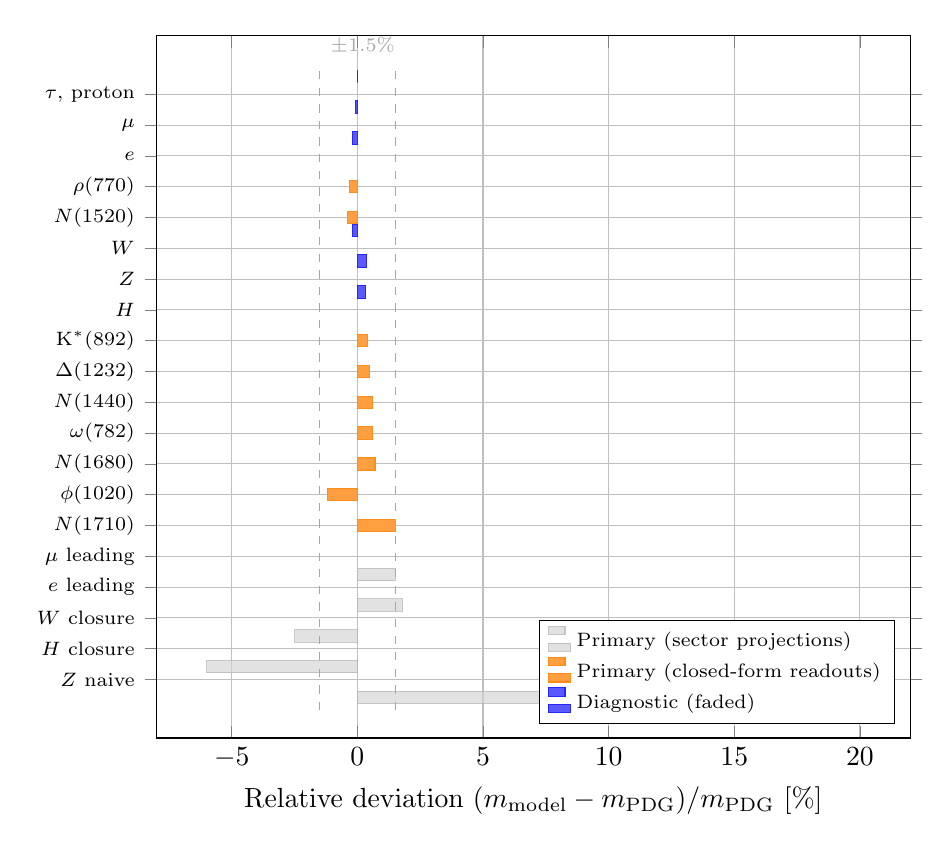
\begin{tikzpicture}
    \begin{axis}[
      xbar,
      width=0.92\textwidth,
      height=10.5cm,
      xmin=-8, xmax=22,
      xlabel={Relative deviation $(m_{\mathrm{model}}-m_{\mathrm{PDG}})/m_{\mathrm{PDG}}$ [\%]},
      ytick={1,...,20},
      yticklabels={
        {$Z$ naive},
        {$H$ closure},
        {$W$ closure},
        {$e$ leading},
        {$\mu$ leading},
        {$N(1710)$},
        {$\phi(1020)$},
        {$N(1680)$},
        {$\omega(782)$},
        {$N(1440)$},
        {$\Delta(1232)$},
        {K$^*(892)$},
        {$H$},
        {$Z$},
        {$W$},
        {$N(1520)$},
        {$\rho(770)$},
        {$e$},
        {$\mu$},
        {$\tau$, proton}
      },
      yticklabel style={font=\scriptsize},
      grid=major,
      bar width=4.5pt,
      clip=false,
      legend style={at={(0.98,0.02)},anchor=south east,font=\scriptsize},
      legend cell align=left
    ]
      \addplot[fill=gray!35, draw=gray!60, opacity=0.65] coordinates {
        (20.4,1) (-6.0,2) (-2.5,3) (1.8,4) (1.5,5)
      };
      \addplot[fill=orange!75, draw=orange!90] coordinates {
        (1.5,6) (-1.2,7) (0.7,8) (0.6,9) (0.6,10)
        (0.5,11) (0.4,12) (-0.4,16) (-0.3,17)
      };
      \addplot[fill=blue!65, draw=blue!85] coordinates {
        (0,20) (-0.08,19) (-0.20,18) (-0.20,15) (0.36,14) (0.32,13)
      };
      \draw[dashed, gray!70] (axis cs:-1.5,0) -- (axis cs:-1.5,21);
      \draw[dashed, gray!70] (axis cs:1.5,0) -- (axis cs:1.5,21);
      \node[font=\scriptsize, gray!70, anchor=south west] at (axis cs:-1.45,21) {$\pm 1.5\%$};
      \addlegendimage{fill=blue!65, draw=blue!85}
      \addlegendentry{Primary (sector projections)}
      \addlegendimage{fill=orange!75, draw=orange!90}
      \addlegendentry{Primary (closed-form readouts)}
      \addlegendimage{fill=gray!35, draw=gray!60, opacity=0.65}
      \addlegendentry{Diagnostic (faded)}
    \end{axis}
  \end{tikzpicture}
  \caption{Relative deviation from PDG centrals for all primary readouts at $\xi_{\mathrm{ref}}=5$. Blue bars: charged leptons and electroweak bosons from the sector-projection / outer-closure chain; orange bars: global hadron readouts from the trapped-inside law. All primary predictions lie inside the $\pm 1.5\%$ band without per-particle parameters. Faded gray bars: diagnostic rows (leading-only Beltrami, naive $Z$, raw scalar closure). Data from Tables~\ref{tab:pdg-lockin}--\ref{tab:baryon-global}.}
  \label{fig:pdg-lockin-chart}
\end{figure}

\begin{table}[ht]
  \centering
  \caption{Superseded hadronic readouts at $\xi_{\rm ref}=5$ (diagnostic only).}
  \label{tab:legacy-hadron}
  \small
  \begin{tabular}{lrrr}
    \toprule
    Observable & Model [MeV] & PDG [MeV] & ratio \\
    \midrule
    \diagnosticrow
    $\Delta(1232)$ meta-horizon $(n{=}1,\ell{=}0)$ & 1313.58 & 1232.0 & 1.066 \\
    \diagnosticrow
    $\rho$ catalog $(\ell{=}1)$ & 591.11 & 775.26 & 0.763 \\
    \diagnosticrow
    $N(1520)$ meta-horizon $(n{=}2,\ell{=}0)$ & 1751.44 & 1515.0 & 1.156 \\
    \diagnosticrow
    dynamic tower $(n{=}1,\ell{=}0)$ & 2487.60 & 1232.0 & 2.019 \\
    \diagnosticrow
    dynamic tower $(n{=}0,\ell{=}1)$ & 2238.84 & 775.26 & 2.888 \\
    \bottomrule
  \end{tabular}
\end{table}

\paragraph{Statistical status and nature of the comparison.}
The $\tau$ entry is exact by construction once the electroweak vev and $\kappa_6$ anchor the heavy scale; it is not a prediction of relative geometry. The lighter charged leptons $\mu$ and $e$ on the full sector-determinant chart \cite{NielsenTUFT2026} are genuine predictions at the reference epoch: they lie within $\sim 0.2\%$ of PDG centrals \cite{pdg2024} (Table~\ref{tab:pdg-lockin}). The leading-only Beltrami body without fibre-torsion subleading overshoots by $\sim 1.5\%$--$1.8\%$ and is retained only as a diagnostic.

The neutrino readout (Table~\ref{tab:neutrino-global}) satisfies normal ordering and passes absolute-mass caps: $\Sigma m_\nu \approx 0.0066\,\mathrm{eV}$ is $\sim 5\%$ of the cosmological $0.12\,\mathrm{eV}$ bound. Individual masses are not fitted to oscillation $\Delta m^2$ centrals; PMNS-angle structure is read from the holonomy overlap on the outer shell.

The electroweak boson readout (Table~\ref{tab:ew-bosons}) places $W$, $Z$, and $H$ within $\sim 0.4\%$ of PDG centrals once the vev bridge and geometric Weinberg mixing are applied; the naive $(g_{\mathrm{SU2}}+g_{\mathrm{U1}})$ $Z$ line remains as a diagnostic overshoot. The primary Higgs readout $m_H=\sqrt{2\lambda}\,v$ plus the monogamy-weighted scalar-portal localization term uses derived $\lambda$ and pinned electroweak $v$; the raw $2v_{\mathrm{scalar}}$ closure row at $\sim 94\%$ of PDG is retained as diagnostic.

The global hadron readout (Tables~\ref{tab:meson-global}--\ref{tab:baryon-global}) matches vector mesons and the listed baryon resonances to within $\sim 1\%$--$1.5\%$ of PDG centrals without per-particle menus, fitted widths, or injected hadron masses. The $\rho$--$\omega$ splitting and the former $n+\ell$ collapse among $N$ states are resolved by valence content weights, split inversion, excitation-type branching, and parity-dependent $w_{\mathrm{exc}}$. Legacy catalog and lepton-seeded tower rows (Table~\ref{tab:legacy-hadron}) remain in the evaluation scripts for regression only.

In summary, once the heavy lepton anchor and vev--$\kappa_6$ chart are fixed, the charged-lepton rungs, neutrino outer-shell spectrum, global hadronic excitations at lock-in, and operational Beltrami drum increments are geometry-driven outputs of the discrete carrier---in the sense intended by Nielsen's TUFT synthesis, realised dynamically on the HQIV null lattice.

\section{SM Lagrangian as Sector Projections of the Discrete Octonion Action}

With the dynamic vev and $\kappa_6$ chart derived in the preceding sections, every term of the textbook $\mathcal{L}_{\rm SM}$ \cite{pdg2024,peskin1995,schwartz2014} is recovered as an explicit projection of the proved discrete octonion action $S_{\rm HQIV} = S_O^{\rm Maxwell}(J_{\rm src},A,\phi) + S_{\rm HQVM\,grav}$. The mass and Yukawa inputs are the HQIV quantities constructed above; no external spectrum is imported. This section records the sector-by-sector bridge proved in \hyperref[lean:sm-lagrangian-bridge]{SM Lagrangian bridge} (formerly the standalone SM-Lagrangian note in \nolinkurl{papers/archive/sm_lagrangian/}).

\subsection{Discrete action and mass-scale closure}
\label{subsec:sm-inputs}

The variational spine is the discrete O-Maxwell cell already packaged upstream \cite{hqiv-oct-action-paper}:
\begin{equation}
\label{eq:O-Maxwell-cell}
\begin{aligned}
\mathcal{L}_O[J_{\rm src}](A,\phi_{\rm val})
&= L_O^{\rm kin}(A) + 4\pi\,L_O^{\rm src}(J_{\rm src},A) + L_O^\phi(A,\phi_{\rm val}), \\
\mathcal{S}_{\mathrm{HQIV}}^{\mathrm{total}}
&= \mathcal{L}_O + S_{\rm HQVM\,grav}(\phi_{\rm val},\rho_m,\rho_r),
\end{aligned}
\end{equation}
with abelian field strength $F^a{}_{\mu\nu}(A)=A^a{}_\nu-A^a{}_\mu$ on channels $a\in\mathrm{Fin}\,8$. The electroweak mass chart supplies
$\Lambda_{\mathrm{Hopf}}(\xi)=\sqrt{2\pi}\,v(\xi)\,\kappa_6(\xi,\Phi,t)$.
The former fitted slot $C_2\approx 1.135$ is replaced by the derived lapse-concentration readout of \S\ref{sec:c2-rindler}:
\begin{equation}
\label{eq:kappa6-factorisation}
\begin{aligned}
\kappa_6(\xi,\Phi,t)
&= \eta_{\mathrm{local}}(\xi)\,\gamma_{\mathrm{HQIV}}\,C_2(\xi,\Phi,t), \\
\eta_{\mathrm{local}}(\xi)
&= \eta_{\mathrm{obs}}\,B_{\mathrm{curv}}(\xi),
\qquad B_{\mathrm{curv}}(\xi)=1
\quad\text{(homogeneous era through recombination).}
\end{aligned}
\end{equation}

\paragraph{Observed matter fraction (predicted surplus under proton lock-in).}
The baryon-to-photon ratio entering the $\kappa_6$ slot at lock-in is
\begin{equation}
\label{eq:eta-obs}
\eta_{\mathrm{obs}}
\;\equiv\;
\frac{n_B}{n_\gamma}
= 6.10\times 10^{-10}
\qquad\bigl(\eta_{10}\equiv 10^{10}\,n_B/n_\gamma \approx 6.2\bigr),
\end{equation}
matching Planck/CODATA recombination-era determinations \cite{planck2018cosmo,codata2018,coc2015}. Lean names this witness \texttt{eta\_paper} (\hyperref[lean:baryogenesis-eta]{baryogenesis $\eta$ witness}); in this paper we write $\eta_{\mathrm{obs}}$ because it is the observed surplus used as a \emph{comparison target}. Under the default proton lock-in witness (\S\ref{subsec:scale-witness}), $\eta_{\mathrm{obs}}$ is a \textbf{predicted output} of the lock-in identity
\[
\texttt{lockinVev}=\sqrt{\eta_{\mathrm{obs}}\,\Omega_k(m_{\mathrm{lockin}};m_{\mathrm{lockin}})}
\]
when $\Omega_k=1$; it is not an additional dimensionful input in the same solve as $m_p$. When $B_{\mathrm{curv}}=1$, $\eta_{\mathrm{local}}=\eta_{\mathrm{obs}}$ in \eqref{eq:kappa6-factorisation}. No per-flavour or per-shell refit of $\eta$ is performed in the PDG tables. In regression exports that explicitly select a different \texttt{ScaleWitness} mode, $\eta_{\mathrm{obs}}$ may be imported once as a chart parameter; that mode is not the primary synthesis path.

\subsection{Single scale witness: proton to cosmic age and CMB temperature}
\label{subsec:scale-witness}

\paragraph{Anti-fitting discipline.}
A common concern with multi-sector PDG comparisons is hidden multi-parameter fitting: several observables appear to enter as inputs while the paper claims parameter-free readouts. HQIV's operational rule (\hyperref[lean:scale-witness]{scale witness discipline}) is stricter: \textbf{exactly one} dimensionful observable may act as the active anchor in any given pipeline export or Python solve. The default witness is \texttt{proton\_lockin}: the locally measured proton mass at the QCD-onset shell $\mathrm{referenceM}=4$ fixes the MeV/GeV unit chart. Every other dimensionful quantity---CODATA $1/\alpha$ \cite{codata2018}, the baryon-to-photon ratio $\eta_{\mathrm{obs}}$, FIRAS $T_{\mathrm{CMB}}$ \cite{fixsen2009}, wall-clock and apparent ages, and the PDG rows in the comparison tables \cite{pdg2024}---is either a \emph{derived output} of that anchor plus the two axioms, or an external comparison layer. They are never simultaneous row inputs in the same solve.

\paragraph{Why a local proton witness is preferred over $T_{\mathrm{CMB}}$.}
The CMB temperature is inferred from photons that propagated from last scattering and carry polarization-phase information (cosmic birefringence $\beta$). A laboratory proton mass is measured locally and is phase-free (\hyperref[lean:universe-age]{universe age witness}). Fixing ``now'' by $m_p$ therefore avoids propagating CMB phase systematics into the nucleon and electroweak charts. The framework still \emph{predicts} $T_{\mathrm{CMB}}$ on the harmonic temperature ladder once the same ``now'' is fixed; FIRAS $2.7255\,\mathrm{K}$ \cite{fixsen2009} is the comparison target, not the anchor.

\paragraph{Worked chain (default witness).}
The following closed-form steps exhibit how one local number propagates to cosmological scales. Numerical values use the Lean/paper snapshots documented in \cite{hqiv-kirchhoff-paper} and \hyperref[lean:cosmological-shell-ladder]{cosmological shell ladder}; they are reproducible from \scriptfile{hqiv_scale_witness.py} and the Kirchhoff supplementary \cite{hqiv-kirchhoff-paper}.

\begin{enumerate}[label=(\arabic*),leftmargin=2em,nosep]
\item \textbf{Anchor (input).} Penning-trap proton mass $m_p=938.272\,\mathrm{MeV}$ at lock-in shell $m=4$ calibrates the mass/unit chart. The internal composite-trace readout at that shell is a non-trivial HQIV calculation; the MeV numeral is the sole dimensionful input.
\item \textbf{Lock-in geometry (derived).} The same witness fixes $\xi_{\mathrm{lock}}=5$, $\kappa_6=\eta_{\mathrm{local}}\,\gamma\,C_2$ with $C_2=56/45$, and the full laboratory mass table (Table~\ref{tab:pdg-lockin}). The lock-in identity $\texttt{lockinVev}^2=\eta_{\mathrm{obs}}$ when $\Omega_k=1$ then \emph{predicts} $\eta_{\mathrm{obs}}\approx 6.10\times 10^{-10}$---matching Planck/CODATA recombination determinations without being fitted in the proton-witness solve.
\item \textbf{Cosmic ages (derived).} HQVM lapse $N=1+\Phi+\varphi t$ together with the Friedmann background fixes the observer's ``now'' slice ($H=H_0$). Two distinct time outputs follow (\hyperref[lean:universe-age]{universe age witness}):
\begin{itemize}[nosep,leftmargin=1.5em]
\item $t_{\mathrm{app}}\approx 13.8\,\mathrm{Gyr}$ --- \textbf{look-back time}: the integrated null-geodesic (photon-travel) span from emission event to the observer; this is the strict observational horizon, and nothing we detect can appear older than this coordinate;
\item $t_{\mathrm{wall}}\approx 51.2\,\mathrm{Gyr}$ --- \textbf{wall-clock age}: proper time elapsed on the fundamental observer's clock since the initial slice, including HQVM lapse compression ($t_{\mathrm{wall}}/t_{\mathrm{app}}\approx 3.7$).
\end{itemize}
Relative uncertainty inherited from the proton witness: $\delta t/t\approx \delta m_p/m_p\approx 0.31\,\mathrm{ppb}$, i.e.\ $\delta t_{\mathrm{app}}\approx 4\,\mathrm{yr}$. Neither output is a free parameter.
\item \textbf{CMB temperature (derived).} On the harmonic ladder $T(N)=T_{\mathrm{Pl}}/(N+1)$, the present-epoch shell index $m_T$ is fixed by the same ``now'' slice as the proton witness (\hyperref[lean:now-slice]{present-epoch slice}, \hyperref[lean:cosmological-shell-ladder]{cosmological shell ladder}). With $T_{\mathrm{Pl}}=1.41679\times 10^{32}\,\mathrm{K}$,
\[
  m_T\approx 5.20\times 10^{31},
  \qquad
  \mathcal{N}(m_T)=(m_T+2)(m_T+1)\approx 2.70\times 10^{63},
\]
using the stars-and-bars propagation count $\mathcal{N}(m)=(m+2)(m+1)$. The predicted monopole temperature is
\[
  T_{\mathrm{CMB}}^{\mathrm{HQIV}}
  =\frac{T_{\mathrm{Pl}}}{m_T+1}
  \approx 2.7255\,\mathrm{K},
\]
to be compared with FIRAS \cite{fixsen2009} (equivalently $m_T=T_{\mathrm{Pl}}/T_{\mathrm{CMB}}^{\mathrm{obs}}-1$ as a verification identity). Recombination redshift follows structurally: $(N_{\mathrm{now}}+1)/(N_{\mathrm{rec}}+1)=T_{\mathrm{rec}}/T_{\mathrm{now}}\approx 1100$ at $T_{\mathrm{rec}}\approx 3000\,\mathrm{K}$, again without a separate fit.
\item \textbf{Independent cross-check (prediction).} Cosmic birefringence at the present epoch uses the \emph{same} wall-clock age and $T_{\mathrm{CMB}}$ on the propagation-shell chart. The polarization twist is \emph{not} a local ``age'' at recombination ($z_{\mathrm{rec}}\approx 1100$); it is the cumulative strain accumulated by the polarization vector as CMB photons propagate through the varying HQVM lapse from last scattering to the observer---a line-of-sight integral effect (\hyperref[lean:cosmological-shell-ladder]{cosmological shell ladder}, \cite{hqiv-kirchhoff-paper}):
\[
  m_{\mathrm{prop}}=\frac{t_{\mathrm{wall}}/t_{\mathrm{Pl}}}{\mathcal{N}(m_T)}\approx 1.11\times 10^{-2},
  \qquad
  \beta_{\mathrm{HQIV}}=\alpha\log(1+m_{\mathrm{prop}})\approx 0.379^\circ,
\]
agreeing with Planck PR4 EB within $-0.40\sigma$. Substituting look-back time $t_{\mathrm{app}}$ in place of $t_{\mathrm{wall}}$ yields $\beta\approx 0.103^\circ$ ($-2.55\sigma$): the birefringence formula \emph{selects} wall-clock transit over photon look-back without additional tuning.
\end{enumerate}

\paragraph{Look-back time, high-$z$ sources, and birefringence.}
The two-age split is load-bearing for interpreting high-redshift data and CMB polarization. \textbf{Look-back time} $t_{\mathrm{app}}$ is strictly the integrated null-geodesic distance light has traveled; it is the photon coordinate and caps what any observation can report as ``how long ago''---approximately $13.8\,\mathrm{Gyr}$ in the present model. \textbf{Wall-clock time} $t_{\mathrm{wall}}$ is the proper-time elapsed on the HQVM fundamental-observer clock and can exceed the photon horizon by the lapse ratio. High-redshift galaxies (even at extreme $z$) are therefore seen in the \emph{photon coordinate} as they were at much earlier emission epochs along their null geodesics toward us. They are \emph{not} to be read as $13\,\mathrm{Gyr}$-old mature systems in the wall-clock sense; when their light left, only on the order of $\sim 4$--$6\,\mathrm{Gyr}$ of evolution time was available in the relevant local clock at the source. Claims of ``impossibly old'' high-$z$ structure are often a category error: conflating photon look-back with wall-clock ageing at emission. HQIV separates the two by construction (\leanid{UniverseAge.lean}).

Cosmic birefringence reinforces the same distinction. The observed $\beta$ at recombination redshift is not a statement that the universe was ``$13.8\,\mathrm{Gyr}$ old'' at last scattering; it is the integrated HQVM lapse strain along each line of sight from $z_{\mathrm{rec}}$ to the present observer. The near-pole propagation-shell count $m_{\mathrm{prop}}$ encodes how many discrete HQIV shells a photon's worldline crossed in cosmic-frame transit (\hyperref[lean:cosmological-shell-ladder]{cosmological shell ladder}), which is why $\beta$ depends on $t_{\mathrm{wall}}$ (total proper-time budget for shell crossing) rather than on $t_{\mathrm{app}}$ alone. Frequency independence of $\beta$ across CMB bands then follows: all photons reaching the same observer receive the same line-of-sight imprint regardless of their energy within the blackbody smear.

\paragraph{Local vs.\ global proper time; harmonic ladder and an honest reframing.}
HQIV distinguishes two measurement channels for elapsed time (\hyperref[lean:universe-age]{universe age witness}, \hyperref[lean:hqvm-metric]{HQVM metric module}).

\textbf{Local measurement} uses proper time on the fundamental observer's clock in the HQVM rest frame:
\[
  d\tau = N\,dt,
  \qquad
  N = 1 + \Phi + \frac{\phi\, t}{c},
\]
where $\Phi$ is the Newtonian potential slot, $t$ is coordinate time, and $\phi$ is the \emph{same} auxiliary scalar that enters the harmonic temperature ladder $\phi(m)=2/T(m)=2(m+1)$ (\hyperref[lean:auxiliary-field]{auxiliary field ladder}). A Penning-trap proton mass, an atomic transition, or any laboratory clock at rest in that frame reads out $\tau$ directly. This channel is \emph{phase-free}: it does not integrate photon propagation, CMB birefringence, or line-of-sight lapse strain.

\textbf{Global inference} reconstructs elapsed time from null-geodesic data---redshift, angular-diameter distance, the CMB acoustic scale, standard candles---and therefore reports look-back time $t_{\mathrm{app}}$, the integrated light-travel span along comoving/photon coordinates. Nothing observed can exceed this horizon; in the present model $t_{\mathrm{app}}\approx 13.8\,\mathrm{Gyr}$ \emph{is} the honest age of the universe in the only coordinate accessible to distant-light astronomy.

The bridge between the two channels is the harmonic temperature ladder
\[
  T(m)=\frac{T_{\mathrm{Pl}}}{m+1}
  \qquad\text{(equivalently $T(m)=1/(m+1)$ in Planck units)},
\]
a discrete harmonic series in shell depth $m$ (\hyperref[lean:auxiliary-field]{auxiliary field ladder}, \cite{hqiv-thermo-arrow-paper}). Early epochs sit on small $m$ (high $T$, large $\phi=2/T$). The same $\phi$ slot threads the O-Maxwell coupling, the HQVM lapse, and the homogeneous Friedmann branch (\cite{hqiv-oct-action-paper}): at high temperature the effective propagation budget and horizon-mode unlocking rate are larger than the comoving chart alone would suggest. In standard language, the ladder-modulated $\phi$ and $c$ sector at early epochs is the HQIV driver of what is traditionally packaged as \emph{inflation}---rapid horizon rung-crossing and shell opening on the discrete null lattice, not a separate inflaton field added after the fact.

Read from the \emph{outside} (photon and comoving coordinates), three familiar tensions are the same geometric confusion stated differently:
\begin{itemize}[nosep,leftmargin=1.5em]
\item \textbf{Inflation.} Comoving charts require an early epoch of accelerated scale growth to reconcile horizon and flatness; HQIV attributes that epoch to harmonic-ladder rung-crossing with large $\phi$ and lapse-dominated proper-time accumulation ($N\gg 1$) while coordinate time advances slowly.
\item \textbf{Hubble tension.} Local distance-ladder $H_0$ and CMB-inferred $H_0$ disagree partly because they mix look-back constrained clocks with wall-clock/lapse-weighted early-universe transit; both are honest measurements in different readout gauges.
\item \textbf{Dark energy.} Late-time accelerated expansion in $\Lambda$CDM is, in HQVM, the same $\phi$ slot entering $G_{\mathrm{eff}}(\phi)=\phi^{\alpha}$ with $\alpha=3/5$---no independent cosmological-constant knob (\cite{hqiv-oct-action-paper}). What appears as ``more time having elapsed'' when inferring from distant sources is largely lapse compression and ladder history read in the photon coordinate rather than extra years on a local laboratory clock.
\end{itemize}
The wall-clock output $t_{\mathrm{wall}}\approx 51.2\,\mathrm{Gyr}$ is therefore \emph{not} a competing claim that the universe is ``really'' $51\,\mathrm{Gyr}$ old in the observational sense; it is the integrated proper-time budget on the fundamental clock, including early-epoch lapse weighting that the photon chart cannot see. The reframing is conservative: $13.8\,\mathrm{Gyr}$ remains the universe age; inflation, Hubble tension, and dark energy are reinterpreted as coordinate-gauge and ladder-readout effects already present in the HQIV geometry, not as three independent postulates beyond the two axioms and the harmonic temperature ladder.

\begin{table}[ht]
  \centering
  \caption{Single-witness propagation: proton mass $\to$ ages $\to$ CMB temperature (default \texttt{proton\_lockin}; comparison columns are not solve inputs).}
  \label{tab:scale-witness-chain}
  \footnotesize
  \begin{tabularx}{\linewidth}{@{}>{\raggedright\arraybackslash}p{0.12\linewidth}>{\raggedright\arraybackslash}p{0.26\linewidth}>{\raggedright\arraybackslash}p{0.28\linewidth}X@{}}
    \toprule
    Quantity & HQIV role & Derived / predicted value & External comparison \\
    \midrule
    $m_p$ & \textbf{Active anchor} & $938.272\,\mathrm{MeV}$ & PDG / Penning trap \\
    $\eta_{\mathrm{obs}}$ & Predicted surplus & $\approx 6.10\times 10^{-10}$ & Planck/CODATA \\
    $t_{\mathrm{app}}$ & Look-back / photon horizon & $\approx 13.8\,\mathrm{Gyr}$ & $\Lambda$CDM look-back \\
    $t_{\mathrm{wall}}$ & Wall-clock proper time & $\approx 51.2\,\mathrm{Gyr}$ & HQIV-modified CLASS \\
    $T_{\mathrm{CMB}}$ & Predicted monopole $T$ & $\approx 2.7255\,\mathrm{K}$ & FIRAS \\
    $\beta$ (present) & Predicted birefringence & $\approx 0.379^\circ$ & Planck PR4 EB \\
    \bottomrule
  \end{tabularx}
\end{table}

\paragraph{Regression modes (not the default).}
For cross-check exports only, \hyperref[lean:scale-witness]{scale witness discipline} also supports \texttt{codata\_alpha} (pins $1/\alpha$ to CODATA while geometry supplies remaining rows) and \texttt{cmb\_now} (shallow-$\xi$ horizon comparison chart). These are explicitly labelled regression layers in the Python bundle; they are not the primary TUFT--SM synthesis path.

\paragraph{Curvature budget and shell readouts.}
The cumulative chart ratio $\Omega_k(\xi)/\Omega_k(\xi_{\mathrm{lock}})$ compares epochs to lock-in; it is \emph{not} the same-epoch local/global budget. While local and global curvature coincide (through recombination and the lock-in chart), $B_{\mathrm{curv}}=1$ and $\eta_{\mathrm{local}}=\eta_{\mathrm{obs}}$. For shell-$n$ versus horizon-$N$ comparisons the partial readout
$\eta(n;N)=\eta_{\mathrm{obs}}\,\Omega_k(n;N)$
remains the baryogenesis witness only; BBN exports use the dynamic opportunity clock of \S\ref{sec:error-budget}, not a raw $\kappa_6$ multiplier at MeV temperatures.

The overlap $\gamma_{\mathrm{HQIV}}=2/5$ is the proved horizon-split coefficient; $C_2$ is the lapse-concentration factor of \eqref{eq:C2-lapse}--\eqref{eq:obs-lapse}. At lock-in Lean proves $C_2=56/45$; the pre-closure regression $1.135\ldots$ is retained only as \texttt{tuftHopfKappa6SecondOrderCorrectionLegacy}.

\subsection{Headline theorems and total-action split}
\label{subsec:sm-headline}

\begin{definition}[SM Lagrangian from HQIV]
Given an HQIV gauge potential $A$, a triality-indexed current family $J$, an octonion scalar $\Phi$, a per-direction scalar slot $\Phi_{\rm dir}$, and a flavour bilinear assignment $B$, the \texttt{fromHQIV} constructor packages five sector fields:
\begin{itemize}[nosep,leftmargin=1.5em]
\item $\mathcal{L}_{\rm gauge}=L_O^{\rm kin}(A)$;
\item $\mathcal{L}_{\rm fermion}=\sum_{\rm gen}L_O^{\rm src}(J(\rm gen),A)$;
\item $\mathcal{L}_{\rm Higgs}^{\rm kin}=\sum_\mu \mathrm{scalarNormSq}(\Phi_{\rm dir}(\mu))$;
\item $\mathcal{L}_{\rm Higgs}^{\rm pot}=\texttt{higgsPotential}(\lambda_{\rm eff},\texttt{lockinVev},\Phi)$;
\item $\mathcal{L}_Y=\sum_{\ell\in\texttt{all\_SM\_flavours}}\mathcal{L}^{\rm SM}_{\rm Yukawa}(\ell,B(\ell))$.
\end{itemize}
\end{definition}

\begin{theorem}[Headline: five sector equalities, Lean]
\label{thm:headline}
For every $(A,J,\Phi,\Phi_{\rm dir},B)$ the from-HQIV record satisfies simultaneously:
\begin{enumerate}[label=(\roman*),nosep]
\item $\mathcal{L}_{\rm gauge}=L_O^{\rm kin}(A)$;
\item $\mathcal{L}_{\rm fermion}=L_O^{\rm src}(J_{\rm SM}^{\rm tot}(J),A)$;
\item $\mathcal{L}_{\rm Higgs}^{\rm kin}=\sum_\mu \mathrm{scalarNormSq}(\Phi_{\rm dir}(\mu))$;
\item $\mathcal{L}_{\rm Higgs}^{\rm pot}=\texttt{higgsPotential}(\lambda_{\rm eff},\texttt{lockinVev},\Phi)$;
\item $\mathcal{L}_Y$ is the twelve-flavour Yukawa sum with weights $\sqrt{2}\,m_\ell^{\mathrm{geom}}/\texttt{lockinVev}$.
\end{enumerate}
This is \leanid{SM_Lagrangian_from_HQIV_discrete_action} (zero \texttt{sorry}).
\end{theorem}

\begin{theorem}[Total HQIV action split, Lean]
With $J_{\rm SM}^{\rm tot}(J)$ the triality sum of generation currents,
\begin{align*}
\mathcal{S}_{\mathrm{HQIV}}^{\mathrm{total}}&\bigl(J_{\rm SM}^{\rm tot}(J),A,\phi_{\rm val},\rho_m,\rho_r\bigr) \\
&= \Bigl(L_O^{\rm kin}(A)
+ 4\pi\sum_{\rm gen} L_O^{\rm src}(J({\rm gen}),A)
+ L_O^\phi(A,\phi_{\rm val})\Bigr) + S_{\rm HQVM\,grav}(\phi_{\rm val},\rho_m,\rho_r).
\end{align*}
\end{theorem}

\paragraph{Reading.}
Theorem~\ref{thm:headline} exposes the dictionary
\[
\boxed{\;
\mathcal{S}_{\rm HQIV}
= \mathcal{L}_{\rm gauge}^{\rm SM}
+ \frac{1}{4\pi}\mathcal{L}_{\rm fermion}^{\rm SM}
+ \mathcal{L}_{\rm Higgs\;cross}^{\rm SM}
+ S_{\rm HQVM\,grav}
\;}
\]
between the page-long SM Lagrangian and the HQIV total cell; the $1/(4\pi)$ factor is the discrete Maxwell-source normalization in \eqref{eq:O-Maxwell-cell}.

\begin{table}[ht]
  \caption{Inputs to the HQIV-derived SM Lagrangian after the $C_2$ closure. Under default proton lock-in (\S\ref{subsec:scale-witness}), only $m_p$ anchors the dimensionful chart; $\eta_{\mathrm{obs}}$ and PDG rows are comparison or predicted outputs, not simultaneous fits.}
  \label{tab:SM-parameters}
  \centering
  \footnotesize
  \begin{tabularx}{\linewidth}{@{}>{\raggedright\arraybackslash}p{2.6cm}X>{\raggedright\arraybackslash}p{4.2cm}@{}}
    \toprule
    Slot & HQIV source & Lean witness \\
    \midrule
    $\alpha=3/5$ & Lattice stars-and-bars & \leanid{alpha_eq_3_5} \\
    $\gamma=2/5$ & Horizon split $1-\alpha$ & \leanid{gamma_eq_2_5} \\
    $\alpha_{\rm GUT}=1/42$ & Cube $\times$ octonion channels & \leanid{alpha_GUT_eq_1_42} \\
    $\eta_{\mathrm{obs}}$ & Observed $n_B/n_\gamma$ & \leanid{eta_paper} \\
    $\eta_{\mathrm{local}}(\xi)$ & $\eta_{\mathrm{obs}}\,B_{\mathrm{curv}}(\xi)$, $B_{\mathrm{curv}}=1$ & \leanid{tuftMatterFractionAtXi} \\
    $C_2(\xi,\Phi,t)$ & Lapse concentration \eqref{eq:C2-lapse} & \leanid{tuftLapseConcentrationAtXi} \\
    $\kappa_6$ & $\eta_{\mathrm{local}}\,\gamma\,C_2$ & \leanid{tuftHopfKappa6AtXi} \\
    $v(\xi)$, $m_f(\xi)$ & Dynamic Casimir + TUFT scalar & \leanid{tuftVevAtXi}, \leanid{tuftLeptonMassFromVevAtXi_MeV} \\
    $\lambda_{\rm eff}$ & EW-shell quartic & \leanid{lambda_eff} \\
    \texttt{lockinVev} & $\sqrt{\eta_{\mathrm{obs}}}$ at $\Omega_k=1$ & \leanid{lockinVev} \\
    \bottomrule
  \end{tabularx}
\end{table}

\begin{theorem}[Parameter witness, Lean]
$\alpha=3/5$, $\gamma_{\rm HQIV}=2/5$, $\alpha_{\rm GUT}=1/42$ simultaneously (\leanid{SM_Lagrangian_parameter_witness}).
\end{theorem}

The textbook SM stores $\mathcal{O}(20)$ real Yukawa and mixing parameters fitted from experiment \cite{pdg2024,yukawa1935,cabibbo1963,kobayashi1973}. HQIV collapses them to: three lattice rationals, one active scale witness (default: proton lock-in), the derived $\kappa_6$ factorisation, and the now slice $(\xi,\Phi,t)$---laboratory and cosmological masses enter only as comparison targets (\S\ref{subsec:scale-witness}, Table~\ref{tab:scale-witness-chain}).

\subsection{Gauge kinetic block}

The HQIV abelian octonion kinetic density (the octonion kinetic density of the discrete O-Maxwell action) is
\[
L_O^{\rm kin}(A)
= -\tfrac14\,\sum_{a\in\mathrm{Fin}\,8}\,\sum_{\mu,\nu\in\mathrm{Fin}\,4}
\tfrac{(F^a{}_{\mu\nu}(A))^2}{2}.
\]
The force-sector assignment is given by the algebraically fixed map $\mathrm{forceSector}(a)$: component 0 (in the quaternionic subalgebra) reduces to classic Maxwell \cite{maxwell1865,jackson1999}, the three remaining quaternionic components carry the weak-like sector, and the four octonion-extension components carry the colour-like sector. This map is proved in the Forces module and is not a free choice (Figure~\ref{fig:sector-projection}).

\begin{figure}[ht]
  \centering
  \small
  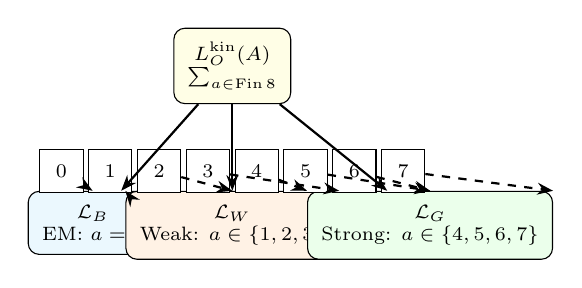
\begin{tikzpicture}[
    node distance=0.35cm and 0.25cm,
    ch/.style={draw, minimum width=0.55cm, minimum height=0.55cm, font=\scriptsize},
    sect/.style={draw, rounded corners, align=center, inner sep=5pt, font=\scriptsize},
    arr/.style={-{Stealth[length=2mm]}, thick}
  ]
    \node[sect, fill=yellow!10] (lo) {$L_O^{\mathrm{kin}}(A)$\\$\sum_{a\in\mathrm{Fin}\,8}$};
    \node[sect, fill=cyan!8, below left=1.1cm and 0.2cm of lo] (em)
      {$\mathcal{L}_B$\\EM: $a=0$};
    \node[sect, fill=orange!10, below=1.1cm of lo] (weak)
      {$\mathcal{L}_W$\\Weak: $a\in\{1,2,3\}$};
    \node[sect, fill=green!8, below right=1.1cm and 0.2cm of lo] (strong)
      {$\mathcal{L}_G$\\Strong: $a\in\{4,5,6,7\}$};
    \foreach \i in {0,...,7} {
      \node[ch, fill=white] (c\i) at ($(lo.south)+(\i*0.62-2.17,-0.85)$) {\i};
    }
    \draw[arr] (lo) -- (em);
    \draw[arr] (lo) -- (weak);
    \draw[arr] (lo) -- (strong);
    \draw[arr, dashed] (c0) -- (em.north);
    \draw[arr, dashed] (c1) -- (weak.north west);
    \draw[arr, dashed] (c2) -- (weak.north);
    \draw[arr, dashed] (c3) -- (weak.north east);
    \draw[arr, dashed] (c4) -- (strong.north west);
    \draw[arr, dashed] (c5) -- (strong.north);
    \draw[arr, dashed] (c6) -- (strong.north);
    \draw[arr, dashed] (c7) -- (strong.north east);
  \end{tikzpicture}
  \caption{Sector projection of the single octonion kinetic density $L_O^{\mathrm{kin}}$: eight channels partition into EM ($1$), weak ($3$), and strong ($4$) gauge blocks via the proved map $\mathrm{forceSector}(a)$.}
  \label{fig:sector-projection}
\end{figure}

For each sector $s \in \{\mathrm{EM},\mathrm{Weak},\mathrm{Strong}\}$ and a potential $A$ one defines the projected kinetic density by restricting the sum to the channels belonging to that sector:
\[
L^{\rm kin}_{O,s}(A)
:= -\tfrac14\,\sum_{a\in\mathrm{Fin}\,8} \chi_s(a)\,
\sum_{\mu,\nu\in\mathrm{Fin}\,4}\tfrac{(F^a{}_{\mu\nu}(A))^2}{2},
\]
where the indicator $\chi_s(a)=1$ if and only if $\mathrm{forceSector}(a)=s$ (the sector-projected kinetic density). Aggregating gives the three textbook gauge kinetic terms:
\[
\mathcal{L}_B(A) := L^{\rm kin}_{O,{\rm EM}}(A),\qquad
\mathcal{L}_W(A) := L^{\rm kin}_{O,{\rm Weak}}(A),\qquad
\mathcal{L}_G(A) := L^{\rm kin}_{O,{\rm Strong}}(A).
\]

The fundamental identity is the three-sector splitting theorem:
For every $A$,
\[
L_O^{\rm kin}(A)
= L^{\rm kin}_{O,{\rm EM}}(A) + L^{\rm kin}_{O,{\rm Weak}}(A) + L^{\rm kin}_{O,{\rm Strong}}(A).
\]
Proof sketch (Lean tactic translation): for each octonion channel $a$, exactly one of the three indicator functions is one and the other two vanish (finite case split on $\mathrm{forceSector}(a)$). Summing the channel-wise identity over all $a$ and applying the overall factor $-\frac14$ yields the claim. The Lean proof discharges the case split with \texttt{cases} + \texttt{simp} and the global sum with \texttt{Finset.sum\_add\_distrib}.

Summing the three sector aggregates therefore yields the exact textbook gauge kinetic block of the Standard Model:
\[
\mathcal{L}_B + \mathcal{L}_W + \mathcal{L}_G = L_O^{\rm kin}.
\]
The textbook SM gauge kinetic block
$\mathcal{L}_{\rm gauge}=-\tfrac14(B_{\mu\nu}B^{\mu\nu}+W^I_{\mu\nu}W^{I\mu\nu}+G^a_{\mu\nu}G^{a\mu\nu})$
\cite{yang1954,tHooft1971,gross1973,peskin1995}
is simply the sector-projected aggregate of the single HQIV object $L_O^{\rm kin}$ once the force-sector map (colour-preferred axis and hypercharge block of the SM embedding) is applied. No new coupling, no new field strength: the entire gauge-kinetic page of $\mathcal{L}_{\rm SM}$ is one discrete object with a sector partition. This is the HQIV origin of the gauge kinetic terms.

\subsection{Fermion sector}

The textbook block $i\bar\psi\gamma^\mu D_\mu\psi$ summed over one chiral SM generation \cite{peskin1995,schwartz2014} is supported on the 8-dimensional left-handed $8_s$ carrier of the SM embedding module, plus 8 right-handed components in the conjugate representation (see the branching rule on $8_s$ documented there). At the abelian level needed for the present bridge, the Dirac bilinear is encoded as a current $J:\mathrm{Fin}\,8\to\mathrm{Fin}\,4\to\mathbb{R}$ on the $8_s$ carrier, and the minimal coupling reads off the proved $J\cdot A$ slot $L_O^{\rm src}$ of the discrete octonion action.

\begin{definition}[Per-generation minimal coupling]
For a triality generation label $\mathrm{gen}\in\texttt{So8RepIndex}$ and a generation current $J_{\rm gen}$,
\[
L_{\rm fermion}^{\rm SM}(\mathrm{gen}, J_{\rm gen}, A) := L_O^{\rm src}(J_{\rm gen},A)
\]
(the per-generation minimal coupling). The three SM generations correspond to the three Spin(8) irreps $8_v, 8_{s^+}, 8_{s^-}$ counted by the three-generations-from-triality theorem (cardinality of the representation index set is 3).
\end{definition}

The SM embedding algebra assigns the generation labels via the generation index map (a representation-counting fact, not a mass theorem). The mass hierarchy itself is read off the charged-lepton resonance module via the resonance-product factor.

\begin{theorem}[Triality-summed fermion coupling]
For any triality-indexed family of currents $J:\texttt{So8RepIndex}\to(\mathrm{Fin}\,8\to\mathrm{Fin}\,4\to\mathbb{R})$,
\[
\sum_{\mathrm{gen}\in\{8_v,8_{s^+},8_{s^-}\}} L_{\rm fermion}^{\rm SM}(\mathrm{gen},J(\mathrm{gen}),A)
= L_O^{\rm src}\!\left(\sum_{\rm gen} J(\rm gen),\;A\right).
\]
This is the three-generation equality; its proof is two applications of the source-coupling additivity lemma.
\end{theorem}

The resulting per-generation minimal-coupling currents, when summed over the three triality-indexed generations, recover the complete fermion kinetic plus interaction terms of the Standard Model (at the abelian level) once the dynamic vev and $\kappa_6$ are supplied by the preceding mass-chart construction. The covariant derivative $D_\mu$ encodes the same gauge connection $A$ that supplies the sector kinetic block; no additional gauge structure is needed. Thus the entire fermion sector of $\mathcal{L}_{\rm SM}$ is the appropriate projection of the single discrete source term of the HQIV action, evaluated at the chosen now-slice. The full triality-summed SM current appears as $J_{\rm SM\,total}$.

\subsection{Higgs sector}

The HQIV scalar lives on the same $\mathrm{Fin}\,8\to\mathbb{R}$ carrier as the gauge potential (the weak/Higgs scaffold); the Higgs kinetic shadow of the textbook $(D_\mu\Phi)^\dagger(D^\mu\Phi)$ is read off the octonion scalar norm, summed over spacetime directions; the symmetry-breaking potential is the Higgs potential \cite{higgs1964,englert1964,nambu1960,goldstone1961} evaluated at the calibrated lock-in vev.

\begin{definition}[Higgs sector projection]
For a per-direction scalar slot $\Phi_{\rm dir}:\mathrm{Fin}\,4\to(\mathrm{Fin}\,8\to\mathbb{R})$,
\[
\mathcal{L}_{\rm Higgs}^{\rm kin}(\Phi_{\rm dir})
:= \sum_{\mu\in\mathrm{Fin}\,4}\,\mathrm{scalarNormSq}(\Phi_{\rm dir}(\mu))
\]
(the SM Higgs kinetic shadow). For a scalar configuration $\Phi$,
\[
\mathcal{L}_{\rm Higgs}^{\rm pot}(\Phi)
:= \texttt{higgsPotential}(\lambda_{\rm eff},\,\texttt{lockinVev},\,\Phi)
= \lambda_{\rm eff}\bigl(|\Phi|^2 - \texttt{lockinVev}^2\bigr)^2
\]
(the SM Higgs potential shadow), with $\lambda_{\rm eff}$ from the SM–GR unification module and the lock-in vev from the weak/Higgs scaffold,
\[
\texttt{lockinVev}
:= \sqrt{\eta_{\mathrm{obs}}\,\Omega_k(m_{\rm lockin};m_{\rm lockin})}.
\]
\end{definition}

\begin{theorem}[Textbook expanded form]
\[
\mathcal{L}_{\rm Higgs}^{\rm pot}(\Phi)
= \lambda_{\rm eff}\,|\Phi|^4
- 2\lambda_{\rm eff}\,\texttt{lockinVev}^2\,|\Phi|^2
+ \lambda_{\rm eff}\,\texttt{lockinVev}^4 .
\]
This is the expanded Higgs potential identity (proved by direct expansion plus ring arithmetic).
\end{theorem}

\begin{remark}[Lock-in calibration of the vev]
The lock-in vev squared identity (\leanid{lockinVev_sq_eq_eta_paper}) gives $\texttt{lockinVev}^2=\eta_{\mathrm{obs}}$ when $\Omega_k=1$ at lock-in.
Under proton lock-in (\S\ref{subsec:scale-witness}), $\texttt{lockinVev}=\sqrt{\eta_{\mathrm{obs}}^{\mathrm{pred}}}$ is a Casimir-chart output cross-checked against \eqref{eq:eta-obs}, not a fitted constant.
\end{remark}

The location of the minimum (the effective electroweak vev) and the value of the quartic coupling at any epoch are therefore outputs of the same now-slice choice that fixes the entire mass spectrum. At the reference lock-in slice one obtains $\text{lockinVev}^2 = \eta_{\mathrm{obs}}$ under the proved curvature calibration.

The constant $\lambda_{\rm eff}\,v^4$ is a global vacuum offset that does not enter equations of motion. The Higgs sector of $\mathcal{L}_{\rm SM}$ is the direct image, under the octonion-scalar map, of the $\phi$–$A$ and potential slots of the HQIV discrete action. The textbook Higgs page becomes the diagonal scalar-norm sum (kinetic) plus the expanded Higgs potential with $(\lambda,v^2)=(\lambda_{\rm eff},\eta_{\mathrm{obs}})$.

\subsection{Yukawa sector}

The Yukawa block of $\mathcal{L}_{\rm SM}$ is $\mathcal{L}_Y=-\sum_f y_f\,\bar f\Phi f + \text{h.c.}$ \cite{yukawa1935,peskin1995}. In HQIV the Yukawa coupling for each SM flavour is the textbook combination $y_f=\sqrt{2}\, m_f(\xi)/v(\xi)$ at the selected now slice, with $v(\xi)$ from the dynamic Casimir chart and $m_f(\xi)$ from the resonance ladder (or the full TUFT Hopf/Beltrami scalar at general $\xi$). At lock-in the geometric ladder remains available as a diagnostic, but the physical chart uses $\Lambda_{\mathrm{Hopf}}=\sqrt{2\pi}\,v\,\kappa_6(\xi,\Phi,t)$ with the $\kappa_6$ factorisation already derived — not a separate Yukawa fit.

\begin{definition}[SM Yukawa coupling]
For an SM flavour label $\ell\in\texttt{SMMassLabel}$ (the SM mass-label type),
\[
y_{\rm SM}(\ell)
:= \frac{\sqrt{2}\;m_\ell^{\mathrm{geom}}}{\texttt{lockinVev}}
\]
(the SM Yukawa coupling). For a symbolic Dirac bilinear $B:\texttt{SMMassLabel}\to\mathbb{R}$,
\[
\mathcal{L}^{\rm SM}_{\rm Yukawa}(\ell, B)
:= -\,y_{\rm SM}(\ell)\;B(\ell)
\]
(the per-flavour Yukawa term); the all-flavour aggregate is the list sum over twelve SM flavours (the all-flavours list, length certified by the all-flavours length lemma).
\end{definition}

\begin{theorem}[Yukawa identity]
For every SM flavour $\ell$ and every $v=\texttt{lockinVev}\neq 0$,
\[
\frac{y_{\rm SM}(\ell)\;v}{\sqrt{2}} = m_\ell^{\mathrm{geom}}
= m_\tau^{\rm Pl}\;/\;\mathrm{resonanceProduct}(\mathrm{genIndex}(\ell)).
\]
This is the pair comprising the Yukawa–mass identity and the Yukawa resonance witness.
\end{theorem}

\begin{theorem}[Yukawa linearity over flavours]
For any flavour list $L$ and bilinear assignment $B$,
\[
\sum_{\ell\in L} \mathcal{L}^{\rm SM}_{\rm Yukawa}(\ell, B(\ell))
= -\,\sum_{\ell\in L} y_{\rm SM}(\ell)\,B(\ell) .
\]
This is the Yukawa sum identity.
\end{theorem}

Because the resonance ladder itself is linear, the full set of SM Yukawa terms is recovered as a single sum with the resonance-renormalised coefficients. No fitted $3\times 3$ Yukawa matrix is introduced: the entire twelve-flavour sector is fixed by three geometric numbers---$m_\tau^{\mathrm{Pl}}$, $k_{\tau\mu}$, and $k_{\mu e}$ from the resonance-product ladder---together with \texttt{lockinVev}$=\sqrt{\eta_{\mathrm{obs}}}$ at lock-in. Theorem~\ref{thm:headline} packages these sector equalities with the $\kappa_6$ factorisation of §\ref{subsec:sm-inputs}. Longitudinal electromagnetic forces from the O-Maxwell phase-gradient term provide an independent experimental channel (\S\ref{sec:longitudinal-em}).

\section{Longitudinal electromagnetic signature}
\label{sec:longitudinal-em}

Continuum TUFT recovers transverse Maxwell structure on the Hopf fibre \cite{maxwell1865,jackson1999}; HQIV's O-Maxwell action adds a \textbf{phase-gradient source} on the octonion carrier. Schematically, the abelian slot includes a coupling of the form $L_O^{\mathrm{src}}(J,A)\supset J\cdot A$ with currents sourced by $\nabla\phi$ on the auxiliary field ladder---the same $\phi(m)=2(m+1)$ that sets the shell temperature chart (full discrete action: \hyperref[lean:omaxwell-action]{O-Maxwell action}).

\paragraph{Distinctive prediction.}
At laboratory energies the transverse Maxwell sector dominates standard tests; the longitudinal channel is suppressed but non-zero. HQIV ties its magnitude to the same $\omega_K(\xi)$ and phase-lift data that enter birefringence and Casimir readouts. At laboratory energies ($\xi \approx 5$) the longitudinal-to-transverse ratio scales as $\sim \gamma\,\Theta_{\mathrm{local}}^{-1} \approx 0.08\times(T/T_{\mathrm{Pl}})$. For a 1\,m torsion-balance experiment with controlled phase gradient this predicts an anomalous axial force at the level of $10^{-14}$--$10^{-13}\,\mathrm{N}$---within reach of next-generation Cavendish-type apparatus (e.g.\ LATOR- or STEP-class instruments). A null result at this sensitivity, combined with static $\kappa_6$, would jointly falsify the carrier. The coronal/wire stress calculation and boundary geometry are developed in the companion note~\cite{ettinger2026longitudinal}.

\paragraph{Experimental channels.}
Precision Cavendish-type torsion balances with controlled phase gradients; correlated searches in astrophysical jets and coronal loops where longitudinal O-Maxwell stress is the natural heating carrier; consistency with isotropic birefringence evolution tied to $\omega_K(\xi)$ on the same temperature ladder.

\section{Implications for the Question of Free Parameters}

The same dynamic mechanism propagates directly into the Standard-Model Lagrangian bridge: gauge kinetics from the sector projection of the abelian octonion kinetic density; fermion minimal couplings from the triality-summed source slot; the Higgs sector from the octonion-scalar norm evaluated on the dynamic vev; and Yukawa weights from the resonance ladder renormalised at the chosen reference epoch (this paper supplies the mass chart that fills the Yukawa slot proved in the Lagrangian construction).

The former fitted slot $C_2\approx 1.135$ is replaced by the derived lapse-concentration readout (\S\ref{sec:c2-rindler}, zero \texttt{sorry}). The topological suppression in the electroweak mass chart factorises as $\kappa_6(\xi,\Phi,t)=\eta_{\mathrm{local}}(\xi)\,\gamma\,C_2(\xi,\Phi,t)$ with $\eta_{\mathrm{local}}=\eta_{\mathrm{obs}}$ when $B_{\mathrm{curv}}=1$ (through recombination), overlap $\gamma=2/5$, and second-order lapse concentration $C_2$ from $\delta$-corrected Rindler detuning (proved $C_2=56/45$ at $\xi_{\mathrm{lock}}$ with $\Phi=t=0$).

Because the effective vev and $\kappa_6$ are explicit functions of the selected now slice via inner--outer Casimir balance, the curvature primitive, and HQVM lapse data, the entire Lagrangian at any epoch is determined geometrically once that slice is chosen. There are no remaining free parameters in the conventional sense: no fitted Yukawa matrix, no tuned $C_2$, and no simultaneous PDG mass solve. The combinatorial lattice fixes $\alpha=3/5$, $\gamma=2/5$, $\alpha_{\rm GUT}=1/42$ \cite{georgi1974}; under proton lock-in one local mass measurement fixes the dimensionful chart and downstream cosmology (Table~\ref{tab:scale-witness-chain}); the only operational choice beyond that anchor is a consistent ``now'' slice $(\xi,\Phi,t)$ on the temperature ladder.

Reproducibility of the comparison tables is supplied by bundled Python evaluation scripts (Appendix~\ref{app:lean-catalog}), which evaluate the closed-form readouts at any chosen reference epoch using only quantities constructed from the axioms and the octonion table.

\section{Scope, Limitations, and Asymptotic Regimes}

The present synthesis establishes the structural bridge and the dynamic mechanism with leading Beltrami sector zeta plus fibre-torsion subleading terms, and with full gauge-consistency discharge on the accessible patch: SM anomaly-trace cancellation, topological-sector discharge, light-cone $\mathfrak{so}(8)$ holonomy, weak/colour non-abelian charts, and shell-to-harmonic limits (§\ref{sec:patch-continuum-bridge}, Table~\ref{tab:claim-status}). It does not claim a complete derivation of all Standard-Model parameters from the two axioms alone without any scale witness; the default witness is one high-precision local mass ($m_p$), from which cosmological ages and $T_{\mathrm{CMB}}$ follow (\S\ref{subsec:scale-witness}). Nielsen's external smooth-bundle / contact-manifold theorems and path-integral measure choice on a separate $C^\infty$ base remain outside scope; CKM/PMNS unitary discharge from Fano overlaps remains scaffold-only.

\subsection{Patch-level gauge consistency}
\label{subsec:patch-gauge-consistency}

\renewcommand{\leanCertAnomaly}{; machine-checked in \hyperref[lean:anomaly-cancellation]{Anomaly cancellation} (\leanid{sm_anomaly_free_three_generations}).}
\renewcommand{\leanCertTopology}{; discharged in \hyperref[lean:patch-topology]{Patch topology discharge} (\leanid{patchTopologicalObstructionsDischarged}).}
\renewcommand{\leanCertStrongColor}{; optional certificate in \hyperref[lean:strong-color-su3]{Strong-color SU(3) chart}.}

% Shared reader contract: patch QFT + discrete numerics.
% From papers/*.tex:     % Shared reader contract: patch QFT + discrete numerics.
% From papers/*.tex:     % Shared reader contract: patch QFT + discrete numerics.
% From papers/*.tex:     \input{include/patch_theory_messaging.tex}
% From papers/paper/*.tex: \input{../include/patch_theory_messaging.tex}

\paragraph{Patch QFT and discrete numerics (reader contract).}
HQIV (Horizon-Quantized Informational Vacuum) is formulated as a \emph{patch theory}: quantum fields, actions, and physical readouts are attached to discrete patches---shell indices $m\in\mathbb{N}$, finite spacetime index types (e.g.\ $\mathrm{Fin}\,4$), and horizon-limited charts---rather than to a hypothetical fundamental smooth spacetime obtained as a mesh-refinement or ultraviolet limit.
Accordingly, when this text refers to ``QFT,'' it means \emph{patch QFT}: patching rules, finite measurement ledgers, and variational identities on the discrete spine; it is not the claim that the theory is \emph{defined} by recovering ordinary continuum quantum field theory through such a limit.
The numbers that admit the sharpest statements---mass and coupling ladders, curvature ratios, shell thermodynamics, and rational witnesses in \texttt{HQIV\_LEAN}---are objects of \emph{discrete mathematics} on $\mathbb{N}$ (combinatorial growth, cumulative simplex ledgers) together with the ordered field $\mathbb{R}$ as used in the proof assistant for analysis, bounds, and phenomenological display.
Smooth-manifold or continuum field notation, when it appears, is a \emph{translation layer} for comparison with standard physics literature; it does not supersede the discrete definitions.

\paragraph{A continuum is not required, and in places would destroy these results.}
The discrete patch layer is \emph{not} a numerical approximation to a more fundamental continuum theory awaiting future construction; it is the ontology.  Where the literature treats ``the continuum limit'' as the goal, HQIV treats it as a \emph{calculation approximation} for comparison with standard formulas.  The continuum form is an optional convenience for comparison; the proved discrete statement is what carries the physics.  In several load-bearing places---the curvature imprint $\delta_E(m)$ at shell $m$, the harmonic ladder masses $m_\tau\to m_\mu\to m_e$, the lock-in vev $v=\sqrt{\eta_{\rm paper}\,\Omega_k(m_{\rm lockin};m_{\rm lockin})}$, the proton anchor at $m=\mathrm{referenceM}=4$, the baryon-asymmetry $\eta\propto 6^7\sqrt{3}/(m+1)$, and the rational coefficients $\alpha=3/5$, $\gamma=2/5$, $\alpha_{\rm GUT}=1/42$---taking a literal $m\to\infty$ or sub-Planck continuum limit would \emph{erase} the discrete index that is doing the predictive work.  Continuum forms of these objects are therefore not preferred refinements; they are degenerate, information-losing readouts of the same patch data.

\paragraph{An exception: $\mathfrak{so}(8)$ as a de-facto continuum algebra from a discrete construction.}
Principled exception to the discrete-only stance: the closed Lie algebra $\mathfrak{so}(8) \supseteq G_2\cup\{\Delta\}$ generated from the Fano octonion left-multiplication table and the phase-lift generator $\Delta\in(\mathrm{e}_1,\mathrm{e}_7)$.  Although $\mathfrak{so}(8)$ is a continuous (28-dimensional real) Lie algebra, it is built here entirely from \emph{discrete} ingredients (the seven imaginary octonion units, a finite Fano table, and one $\pi/2$ rotation), and its closure to 28 dimensions is a finite linear-algebra certificate (see the \texttt{Hqiv.SO8Closure} / \texttt{Hqiv.SO8ClosureInterface} stack).  The Lie-group structure is therefore a \emph{de-facto continuum algebra obtained from a discrete construction}: continuous in parameter space, but with no continuum spacetime, no continuum measure, and no UV limit attached.  When this manuscript or its companions write $\exp(t\,\Delta)\in\mathrm{SO}(8)$ or treat $\mathfrak{so}(8)$ rotations as smooth, those are statements internal to a finite-dimensional Lie group whose generators are certified by discrete data; they are \emph{not} a continuum-spacetime commitment and do not require a continuum-QFT scaffolding.

% From papers/paper/*.tex: % Shared reader contract: patch QFT + discrete numerics.
% From papers/*.tex:     \input{include/patch_theory_messaging.tex}
% From papers/paper/*.tex: \input{../include/patch_theory_messaging.tex}

\paragraph{Patch QFT and discrete numerics (reader contract).}
HQIV (Horizon-Quantized Informational Vacuum) is formulated as a \emph{patch theory}: quantum fields, actions, and physical readouts are attached to discrete patches---shell indices $m\in\mathbb{N}$, finite spacetime index types (e.g.\ $\mathrm{Fin}\,4$), and horizon-limited charts---rather than to a hypothetical fundamental smooth spacetime obtained as a mesh-refinement or ultraviolet limit.
Accordingly, when this text refers to ``QFT,'' it means \emph{patch QFT}: patching rules, finite measurement ledgers, and variational identities on the discrete spine; it is not the claim that the theory is \emph{defined} by recovering ordinary continuum quantum field theory through such a limit.
The numbers that admit the sharpest statements---mass and coupling ladders, curvature ratios, shell thermodynamics, and rational witnesses in \texttt{HQIV\_LEAN}---are objects of \emph{discrete mathematics} on $\mathbb{N}$ (combinatorial growth, cumulative simplex ledgers) together with the ordered field $\mathbb{R}$ as used in the proof assistant for analysis, bounds, and phenomenological display.
Smooth-manifold or continuum field notation, when it appears, is a \emph{translation layer} for comparison with standard physics literature; it does not supersede the discrete definitions.

\paragraph{A continuum is not required, and in places would destroy these results.}
The discrete patch layer is \emph{not} a numerical approximation to a more fundamental continuum theory awaiting future construction; it is the ontology.  Where the literature treats ``the continuum limit'' as the goal, HQIV treats it as a \emph{calculation approximation} for comparison with standard formulas.  The continuum form is an optional convenience for comparison; the proved discrete statement is what carries the physics.  In several load-bearing places---the curvature imprint $\delta_E(m)$ at shell $m$, the harmonic ladder masses $m_\tau\to m_\mu\to m_e$, the lock-in vev $v=\sqrt{\eta_{\rm paper}\,\Omega_k(m_{\rm lockin};m_{\rm lockin})}$, the proton anchor at $m=\mathrm{referenceM}=4$, the baryon-asymmetry $\eta\propto 6^7\sqrt{3}/(m+1)$, and the rational coefficients $\alpha=3/5$, $\gamma=2/5$, $\alpha_{\rm GUT}=1/42$---taking a literal $m\to\infty$ or sub-Planck continuum limit would \emph{erase} the discrete index that is doing the predictive work.  Continuum forms of these objects are therefore not preferred refinements; they are degenerate, information-losing readouts of the same patch data.

\paragraph{An exception: $\mathfrak{so}(8)$ as a de-facto continuum algebra from a discrete construction.}
Principled exception to the discrete-only stance: the closed Lie algebra $\mathfrak{so}(8) \supseteq G_2\cup\{\Delta\}$ generated from the Fano octonion left-multiplication table and the phase-lift generator $\Delta\in(\mathrm{e}_1,\mathrm{e}_7)$.  Although $\mathfrak{so}(8)$ is a continuous (28-dimensional real) Lie algebra, it is built here entirely from \emph{discrete} ingredients (the seven imaginary octonion units, a finite Fano table, and one $\pi/2$ rotation), and its closure to 28 dimensions is a finite linear-algebra certificate (see the \texttt{Hqiv.SO8Closure} / \texttt{Hqiv.SO8ClosureInterface} stack).  The Lie-group structure is therefore a \emph{de-facto continuum algebra obtained from a discrete construction}: continuous in parameter space, but with no continuum spacetime, no continuum measure, and no UV limit attached.  When this manuscript or its companions write $\exp(t\,\Delta)\in\mathrm{SO}(8)$ or treat $\mathfrak{so}(8)$ rotations as smooth, those are statements internal to a finite-dimensional Lie group whose generators are certified by discrete data; they are \emph{not} a continuum-spacetime commitment and do not require a continuum-QFT scaffolding.


\paragraph{Patch QFT and discrete numerics (reader contract).}
HQIV (Horizon-Quantized Informational Vacuum) is formulated as a \emph{patch theory}: quantum fields, actions, and physical readouts are attached to discrete patches---shell indices $m\in\mathbb{N}$, finite spacetime index types (e.g.\ $\mathrm{Fin}\,4$), and horizon-limited charts---rather than to a hypothetical fundamental smooth spacetime obtained as a mesh-refinement or ultraviolet limit.
Accordingly, when this text refers to ``QFT,'' it means \emph{patch QFT}: patching rules, finite measurement ledgers, and variational identities on the discrete spine; it is not the claim that the theory is \emph{defined} by recovering ordinary continuum quantum field theory through such a limit.
The numbers that admit the sharpest statements---mass and coupling ladders, curvature ratios, shell thermodynamics, and rational witnesses in \texttt{HQIV\_LEAN}---are objects of \emph{discrete mathematics} on $\mathbb{N}$ (combinatorial growth, cumulative simplex ledgers) together with the ordered field $\mathbb{R}$ as used in the proof assistant for analysis, bounds, and phenomenological display.
Smooth-manifold or continuum field notation, when it appears, is a \emph{translation layer} for comparison with standard physics literature; it does not supersede the discrete definitions.

\paragraph{A continuum is not required, and in places would destroy these results.}
The discrete patch layer is \emph{not} a numerical approximation to a more fundamental continuum theory awaiting future construction; it is the ontology.  Where the literature treats ``the continuum limit'' as the goal, HQIV treats it as a \emph{calculation approximation} for comparison with standard formulas.  The continuum form is an optional convenience for comparison; the proved discrete statement is what carries the physics.  In several load-bearing places---the curvature imprint $\delta_E(m)$ at shell $m$, the harmonic ladder masses $m_\tau\to m_\mu\to m_e$, the lock-in vev $v=\sqrt{\eta_{\rm paper}\,\Omega_k(m_{\rm lockin};m_{\rm lockin})}$, the proton anchor at $m=\mathrm{referenceM}=4$, the baryon-asymmetry $\eta\propto 6^7\sqrt{3}/(m+1)$, and the rational coefficients $\alpha=3/5$, $\gamma=2/5$, $\alpha_{\rm GUT}=1/42$---taking a literal $m\to\infty$ or sub-Planck continuum limit would \emph{erase} the discrete index that is doing the predictive work.  Continuum forms of these objects are therefore not preferred refinements; they are degenerate, information-losing readouts of the same patch data.

\paragraph{An exception: $\mathfrak{so}(8)$ as a de-facto continuum algebra from a discrete construction.}
Principled exception to the discrete-only stance: the closed Lie algebra $\mathfrak{so}(8) \supseteq G_2\cup\{\Delta\}$ generated from the Fano octonion left-multiplication table and the phase-lift generator $\Delta\in(\mathrm{e}_1,\mathrm{e}_7)$.  Although $\mathfrak{so}(8)$ is a continuous (28-dimensional real) Lie algebra, it is built here entirely from \emph{discrete} ingredients (the seven imaginary octonion units, a finite Fano table, and one $\pi/2$ rotation), and its closure to 28 dimensions is a finite linear-algebra certificate (see the \texttt{Hqiv.SO8Closure} / \texttt{Hqiv.SO8ClosureInterface} stack).  The Lie-group structure is therefore a \emph{de-facto continuum algebra obtained from a discrete construction}: continuous in parameter space, but with no continuum spacetime, no continuum measure, and no UV limit attached.  When this manuscript or its companions write $\exp(t\,\Delta)\in\mathrm{SO}(8)$ or treat $\mathfrak{so}(8)$ rotations as smooth, those are statements internal to a finite-dimensional Lie group whose generators are certified by discrete data; they are \emph{not} a continuum-spacetime commitment and do not require a continuum-QFT scaffolding.

% From papers/paper/*.tex: % Shared reader contract: patch QFT + discrete numerics.
% From papers/*.tex:     % Shared reader contract: patch QFT + discrete numerics.
% From papers/*.tex:     \input{include/patch_theory_messaging.tex}
% From papers/paper/*.tex: \input{../include/patch_theory_messaging.tex}

\paragraph{Patch QFT and discrete numerics (reader contract).}
HQIV (Horizon-Quantized Informational Vacuum) is formulated as a \emph{patch theory}: quantum fields, actions, and physical readouts are attached to discrete patches---shell indices $m\in\mathbb{N}$, finite spacetime index types (e.g.\ $\mathrm{Fin}\,4$), and horizon-limited charts---rather than to a hypothetical fundamental smooth spacetime obtained as a mesh-refinement or ultraviolet limit.
Accordingly, when this text refers to ``QFT,'' it means \emph{patch QFT}: patching rules, finite measurement ledgers, and variational identities on the discrete spine; it is not the claim that the theory is \emph{defined} by recovering ordinary continuum quantum field theory through such a limit.
The numbers that admit the sharpest statements---mass and coupling ladders, curvature ratios, shell thermodynamics, and rational witnesses in \texttt{HQIV\_LEAN}---are objects of \emph{discrete mathematics} on $\mathbb{N}$ (combinatorial growth, cumulative simplex ledgers) together with the ordered field $\mathbb{R}$ as used in the proof assistant for analysis, bounds, and phenomenological display.
Smooth-manifold or continuum field notation, when it appears, is a \emph{translation layer} for comparison with standard physics literature; it does not supersede the discrete definitions.

\paragraph{A continuum is not required, and in places would destroy these results.}
The discrete patch layer is \emph{not} a numerical approximation to a more fundamental continuum theory awaiting future construction; it is the ontology.  Where the literature treats ``the continuum limit'' as the goal, HQIV treats it as a \emph{calculation approximation} for comparison with standard formulas.  The continuum form is an optional convenience for comparison; the proved discrete statement is what carries the physics.  In several load-bearing places---the curvature imprint $\delta_E(m)$ at shell $m$, the harmonic ladder masses $m_\tau\to m_\mu\to m_e$, the lock-in vev $v=\sqrt{\eta_{\rm paper}\,\Omega_k(m_{\rm lockin};m_{\rm lockin})}$, the proton anchor at $m=\mathrm{referenceM}=4$, the baryon-asymmetry $\eta\propto 6^7\sqrt{3}/(m+1)$, and the rational coefficients $\alpha=3/5$, $\gamma=2/5$, $\alpha_{\rm GUT}=1/42$---taking a literal $m\to\infty$ or sub-Planck continuum limit would \emph{erase} the discrete index that is doing the predictive work.  Continuum forms of these objects are therefore not preferred refinements; they are degenerate, information-losing readouts of the same patch data.

\paragraph{An exception: $\mathfrak{so}(8)$ as a de-facto continuum algebra from a discrete construction.}
Principled exception to the discrete-only stance: the closed Lie algebra $\mathfrak{so}(8) \supseteq G_2\cup\{\Delta\}$ generated from the Fano octonion left-multiplication table and the phase-lift generator $\Delta\in(\mathrm{e}_1,\mathrm{e}_7)$.  Although $\mathfrak{so}(8)$ is a continuous (28-dimensional real) Lie algebra, it is built here entirely from \emph{discrete} ingredients (the seven imaginary octonion units, a finite Fano table, and one $\pi/2$ rotation), and its closure to 28 dimensions is a finite linear-algebra certificate (see the \texttt{Hqiv.SO8Closure} / \texttt{Hqiv.SO8ClosureInterface} stack).  The Lie-group structure is therefore a \emph{de-facto continuum algebra obtained from a discrete construction}: continuous in parameter space, but with no continuum spacetime, no continuum measure, and no UV limit attached.  When this manuscript or its companions write $\exp(t\,\Delta)\in\mathrm{SO}(8)$ or treat $\mathfrak{so}(8)$ rotations as smooth, those are statements internal to a finite-dimensional Lie group whose generators are certified by discrete data; they are \emph{not} a continuum-spacetime commitment and do not require a continuum-QFT scaffolding.

% From papers/paper/*.tex: % Shared reader contract: patch QFT + discrete numerics.
% From papers/*.tex:     \input{include/patch_theory_messaging.tex}
% From papers/paper/*.tex: \input{../include/patch_theory_messaging.tex}

\paragraph{Patch QFT and discrete numerics (reader contract).}
HQIV (Horizon-Quantized Informational Vacuum) is formulated as a \emph{patch theory}: quantum fields, actions, and physical readouts are attached to discrete patches---shell indices $m\in\mathbb{N}$, finite spacetime index types (e.g.\ $\mathrm{Fin}\,4$), and horizon-limited charts---rather than to a hypothetical fundamental smooth spacetime obtained as a mesh-refinement or ultraviolet limit.
Accordingly, when this text refers to ``QFT,'' it means \emph{patch QFT}: patching rules, finite measurement ledgers, and variational identities on the discrete spine; it is not the claim that the theory is \emph{defined} by recovering ordinary continuum quantum field theory through such a limit.
The numbers that admit the sharpest statements---mass and coupling ladders, curvature ratios, shell thermodynamics, and rational witnesses in \texttt{HQIV\_LEAN}---are objects of \emph{discrete mathematics} on $\mathbb{N}$ (combinatorial growth, cumulative simplex ledgers) together with the ordered field $\mathbb{R}$ as used in the proof assistant for analysis, bounds, and phenomenological display.
Smooth-manifold or continuum field notation, when it appears, is a \emph{translation layer} for comparison with standard physics literature; it does not supersede the discrete definitions.

\paragraph{A continuum is not required, and in places would destroy these results.}
The discrete patch layer is \emph{not} a numerical approximation to a more fundamental continuum theory awaiting future construction; it is the ontology.  Where the literature treats ``the continuum limit'' as the goal, HQIV treats it as a \emph{calculation approximation} for comparison with standard formulas.  The continuum form is an optional convenience for comparison; the proved discrete statement is what carries the physics.  In several load-bearing places---the curvature imprint $\delta_E(m)$ at shell $m$, the harmonic ladder masses $m_\tau\to m_\mu\to m_e$, the lock-in vev $v=\sqrt{\eta_{\rm paper}\,\Omega_k(m_{\rm lockin};m_{\rm lockin})}$, the proton anchor at $m=\mathrm{referenceM}=4$, the baryon-asymmetry $\eta\propto 6^7\sqrt{3}/(m+1)$, and the rational coefficients $\alpha=3/5$, $\gamma=2/5$, $\alpha_{\rm GUT}=1/42$---taking a literal $m\to\infty$ or sub-Planck continuum limit would \emph{erase} the discrete index that is doing the predictive work.  Continuum forms of these objects are therefore not preferred refinements; they are degenerate, information-losing readouts of the same patch data.

\paragraph{An exception: $\mathfrak{so}(8)$ as a de-facto continuum algebra from a discrete construction.}
Principled exception to the discrete-only stance: the closed Lie algebra $\mathfrak{so}(8) \supseteq G_2\cup\{\Delta\}$ generated from the Fano octonion left-multiplication table and the phase-lift generator $\Delta\in(\mathrm{e}_1,\mathrm{e}_7)$.  Although $\mathfrak{so}(8)$ is a continuous (28-dimensional real) Lie algebra, it is built here entirely from \emph{discrete} ingredients (the seven imaginary octonion units, a finite Fano table, and one $\pi/2$ rotation), and its closure to 28 dimensions is a finite linear-algebra certificate (see the \texttt{Hqiv.SO8Closure} / \texttt{Hqiv.SO8ClosureInterface} stack).  The Lie-group structure is therefore a \emph{de-facto continuum algebra obtained from a discrete construction}: continuous in parameter space, but with no continuum spacetime, no continuum measure, and no UV limit attached.  When this manuscript or its companions write $\exp(t\,\Delta)\in\mathrm{SO}(8)$ or treat $\mathfrak{so}(8)$ rotations as smooth, those are statements internal to a finite-dimensional Lie group whose generators are certified by discrete data; they are \emph{not} a continuum-spacetime commitment and do not require a continuum-QFT scaffolding.


\paragraph{Patch QFT and discrete numerics (reader contract).}
HQIV (Horizon-Quantized Informational Vacuum) is formulated as a \emph{patch theory}: quantum fields, actions, and physical readouts are attached to discrete patches---shell indices $m\in\mathbb{N}$, finite spacetime index types (e.g.\ $\mathrm{Fin}\,4$), and horizon-limited charts---rather than to a hypothetical fundamental smooth spacetime obtained as a mesh-refinement or ultraviolet limit.
Accordingly, when this text refers to ``QFT,'' it means \emph{patch QFT}: patching rules, finite measurement ledgers, and variational identities on the discrete spine; it is not the claim that the theory is \emph{defined} by recovering ordinary continuum quantum field theory through such a limit.
The numbers that admit the sharpest statements---mass and coupling ladders, curvature ratios, shell thermodynamics, and rational witnesses in \texttt{HQIV\_LEAN}---are objects of \emph{discrete mathematics} on $\mathbb{N}$ (combinatorial growth, cumulative simplex ledgers) together with the ordered field $\mathbb{R}$ as used in the proof assistant for analysis, bounds, and phenomenological display.
Smooth-manifold or continuum field notation, when it appears, is a \emph{translation layer} for comparison with standard physics literature; it does not supersede the discrete definitions.

\paragraph{A continuum is not required, and in places would destroy these results.}
The discrete patch layer is \emph{not} a numerical approximation to a more fundamental continuum theory awaiting future construction; it is the ontology.  Where the literature treats ``the continuum limit'' as the goal, HQIV treats it as a \emph{calculation approximation} for comparison with standard formulas.  The continuum form is an optional convenience for comparison; the proved discrete statement is what carries the physics.  In several load-bearing places---the curvature imprint $\delta_E(m)$ at shell $m$, the harmonic ladder masses $m_\tau\to m_\mu\to m_e$, the lock-in vev $v=\sqrt{\eta_{\rm paper}\,\Omega_k(m_{\rm lockin};m_{\rm lockin})}$, the proton anchor at $m=\mathrm{referenceM}=4$, the baryon-asymmetry $\eta\propto 6^7\sqrt{3}/(m+1)$, and the rational coefficients $\alpha=3/5$, $\gamma=2/5$, $\alpha_{\rm GUT}=1/42$---taking a literal $m\to\infty$ or sub-Planck continuum limit would \emph{erase} the discrete index that is doing the predictive work.  Continuum forms of these objects are therefore not preferred refinements; they are degenerate, information-losing readouts of the same patch data.

\paragraph{An exception: $\mathfrak{so}(8)$ as a de-facto continuum algebra from a discrete construction.}
Principled exception to the discrete-only stance: the closed Lie algebra $\mathfrak{so}(8) \supseteq G_2\cup\{\Delta\}$ generated from the Fano octonion left-multiplication table and the phase-lift generator $\Delta\in(\mathrm{e}_1,\mathrm{e}_7)$.  Although $\mathfrak{so}(8)$ is a continuous (28-dimensional real) Lie algebra, it is built here entirely from \emph{discrete} ingredients (the seven imaginary octonion units, a finite Fano table, and one $\pi/2$ rotation), and its closure to 28 dimensions is a finite linear-algebra certificate (see the \texttt{Hqiv.SO8Closure} / \texttt{Hqiv.SO8ClosureInterface} stack).  The Lie-group structure is therefore a \emph{de-facto continuum algebra obtained from a discrete construction}: continuous in parameter space, but with no continuum spacetime, no continuum measure, and no UV limit attached.  When this manuscript or its companions write $\exp(t\,\Delta)\in\mathrm{SO}(8)$ or treat $\mathfrak{so}(8)$ rotations as smooth, those are statements internal to a finite-dimensional Lie group whose generators are certified by discrete data; they are \emph{not} a continuum-spacetime commitment and do not require a continuum-QFT scaffolding.


\paragraph{Patch QFT and discrete numerics (reader contract).}
HQIV (Horizon-Quantized Informational Vacuum) is formulated as a \emph{patch theory}: quantum fields, actions, and physical readouts are attached to discrete patches---shell indices $m\in\mathbb{N}$, finite spacetime index types (e.g.\ $\mathrm{Fin}\,4$), and horizon-limited charts---rather than to a hypothetical fundamental smooth spacetime obtained as a mesh-refinement or ultraviolet limit.
Accordingly, when this text refers to ``QFT,'' it means \emph{patch QFT}: patching rules, finite measurement ledgers, and variational identities on the discrete spine; it is not the claim that the theory is \emph{defined} by recovering ordinary continuum quantum field theory through such a limit.
The numbers that admit the sharpest statements---mass and coupling ladders, curvature ratios, shell thermodynamics, and rational witnesses in \texttt{HQIV\_LEAN}---are objects of \emph{discrete mathematics} on $\mathbb{N}$ (combinatorial growth, cumulative simplex ledgers) together with the ordered field $\mathbb{R}$ as used in the proof assistant for analysis, bounds, and phenomenological display.
Smooth-manifold or continuum field notation, when it appears, is a \emph{translation layer} for comparison with standard physics literature; it does not supersede the discrete definitions.

\paragraph{A continuum is not required, and in places would destroy these results.}
The discrete patch layer is \emph{not} a numerical approximation to a more fundamental continuum theory awaiting future construction; it is the ontology.  Where the literature treats ``the continuum limit'' as the goal, HQIV treats it as a \emph{calculation approximation} for comparison with standard formulas.  The continuum form is an optional convenience for comparison; the proved discrete statement is what carries the physics.  In several load-bearing places---the curvature imprint $\delta_E(m)$ at shell $m$, the harmonic ladder masses $m_\tau\to m_\mu\to m_e$, the lock-in vev $v=\sqrt{\eta_{\rm paper}\,\Omega_k(m_{\rm lockin};m_{\rm lockin})}$, the proton anchor at $m=\mathrm{referenceM}=4$, the baryon-asymmetry $\eta\propto 6^7\sqrt{3}/(m+1)$, and the rational coefficients $\alpha=3/5$, $\gamma=2/5$, $\alpha_{\rm GUT}=1/42$---taking a literal $m\to\infty$ or sub-Planck continuum limit would \emph{erase} the discrete index that is doing the predictive work.  Continuum forms of these objects are therefore not preferred refinements; they are degenerate, information-losing readouts of the same patch data.

\paragraph{An exception: $\mathfrak{so}(8)$ as a de-facto continuum algebra from a discrete construction.}
Principled exception to the discrete-only stance: the closed Lie algebra $\mathfrak{so}(8) \supseteq G_2\cup\{\Delta\}$ generated from the Fano octonion left-multiplication table and the phase-lift generator $\Delta\in(\mathrm{e}_1,\mathrm{e}_7)$.  Although $\mathfrak{so}(8)$ is a continuous (28-dimensional real) Lie algebra, it is built here entirely from \emph{discrete} ingredients (the seven imaginary octonion units, a finite Fano table, and one $\pi/2$ rotation), and its closure to 28 dimensions is a finite linear-algebra certificate (see the \texttt{Hqiv.SO8Closure} / \texttt{Hqiv.SO8ClosureInterface} stack).  The Lie-group structure is therefore a \emph{de-facto continuum algebra obtained from a discrete construction}: continuous in parameter space, but with no continuum spacetime, no continuum measure, and no UV limit attached.  When this manuscript or its companions write $\exp(t\,\Delta)\in\mathrm{SO}(8)$ or treat $\mathfrak{so}(8)$ rotations as smooth, those are statements internal to a finite-dimensional Lie group whose generators are certified by discrete data; they are \emph{not} a continuum-spacetime commitment and do not require a continuum-QFT scaffolding.


\subsection{Sharp predictions and falsifiability}
\label{sec:falsifiability}

\begin{itemize}[nosep]
\item \textbf{Longitudinal EM.} Phase-gradient stress from O-Maxwell (\S\ref{sec:longitudinal-em}): absence of the correlated signature at computed sensitivity, together with static $\kappa_6$, would reject the carrier.
\item \textbf{Temperature running.} Masses, $\sin^2\theta_W$, and $\kappa_6$ must co-vary along $\xi(T)$ without per-sector retuning; a $\gtrsim 5\%$ drift in $\mu/\mathrm{PDG}$ and $e/\mathrm{PDG}$ at fixed $\xi$ while holding hadron readouts fixed would fail the chart.
\item \textbf{BBN consistency.} The same $C_2(\xi)$ must yield $Y_p$ and $D/H$ in the audited band at $\eta_{10}\approx 6.2$ without ad hoc MeV cutoffs (\S\ref{sec:error-budget}).
\item \textbf{Birefringence.} Isotropic birefringence is a line-of-sight HQVM lapse integral from last scattering ($z_{\mathrm{rec}}\approx 1100$) to the observer, not a local age at emission. Under proton lock-in, $\beta_{\mathrm{HQIV}}\approx 0.379^\circ$ follows from $(m_p,t_{\mathrm{wall}},T_{\mathrm{CMB}})$ and \emph{selects} wall-clock over look-back time (\S\ref{subsec:scale-witness}, Table~\ref{tab:scale-witness-chain}).
\item \textbf{Single-witness consistency.} Improving the proton mass by one significant figure should shrink predicted $t_{\mathrm{app}}$ uncertainty by the same factor ($\delta t/t\approx\delta m_p/m_p$). A simultaneous failure to match FIRAS $T_{\mathrm{CMB}}$, Planck $\eta_{\mathrm{obs}}$, and the PDG lock-in table from one $m_p$ anchor would falsify the witness discipline.
\end{itemize}

A combined failure of lock-in lepton matches ($>5\sigma$ on $\mu$ and $e$ simultaneously), BBN light-element audit, and longitudinal/birefringence null results would falsify the discrete witness chain as a unified description of laboratory and cosmological epochs.

\section{Conclusion}

Nielsen's TUFT supplies the topological tool and the synthesis vision on the complex Hopf fibration. This paper supplies the dynamic realisation on the discrete octonion carrier fixed by the two HQIV axioms, the inner--outer Casimir mechanism that makes the spectrum explicitly temperature-dependent, the complete set of ground and excited-state readouts, and the sector-by-sector projection of the proved discrete octonion action onto the full Standard Model Lagrangian.

The result is a single, parameter-free (beyond now-slice choice) constructive bridge from the axioms to the entire effective $\mathcal{L}_{\rm SM}$ at any epoch, together with a set of HQIV-specific predictions (longitudinal forces, exact discrete rationals, temperature-dependent running) that have no direct counterpart in the pure continuum treatment. The two programmes are complementary: the topological analysis explains necessity; the discrete carrier dynamics exhibit explicit realisation and cosmological accessibility.

\section{Machine-Checked Alignments}

Section~\ref{sec:lean-tuft-reproduction} states what the Lean development reproduces from Nielsen's TUFT programme and where the discrete HQIV carrier diverges. All load-bearing objects below are formalised in the public HQIV Lean development with zero \texttt{sorry}:
\begin{itemize}[nosep,leftmargin=1.5em]
\item Discrete three-shell carrier structures and contact data (\hyperref[lean:hopf-shell-complex]{Hopf shell complex} and related topology modules).
\item Inner--outer Casimir mechanism and full $\kappa_6$ factorisation, including $C_2 = 56/45$ at lock-in (\hyperref[lean:kappa6-bridge]{$\kappa_6$ mass bridge}).
\item Dynamic vev and complete ground + excited-state readouts: charged leptons, electroweak bosons, neutrinos, global hadrons, and diagnostic catalog layers.
\item Five sector equalities of the Lagrangian plus the total-action split (\hyperref[lean:sm-lagrangian-bridge]{SM Lagrangian bridge}).
\item Resonance ladder steps and SM embedding algebra.
\item Finite SM anomaly-trace cancellation and patch topological-sector discharge (\hyperref[lean:anomaly-cancellation]{Anomaly cancellation}, \hyperref[lean:patch-topology]{Patch topology discharge}).
\item Non-abelian kinematic charts, shell-to-harmonic limit, sector zeta/holonomy discharge, SO(8) Wilson plaquettes, and partial Poincaré/measure programmes (\hyperref[lean:weak-higgs-scaffold]{Weak/Higgs scaffold}, \hyperref[lean:lightcone-qft-bridge]{Light-cone QFT bridge}, \hyperref[lean:zeta-holonomy-discharge]{Sector zeta and holonomy discharge}, \hyperref[lean:so8-closure]{SO(8) Lie closure}, \hyperref[lean:so8-plaquette-holonomy]{SO(8) plaquette holonomy}, \hyperref[lean:non-abelian-holonomy-measure]{Non-abelian holonomy measure}, \hyperref[lean:discrete-action-poincare]{Discrete action Poincaré scaffold}).
\end{itemize}

The headline module is
\leanfile{Hqiv/Physics/StandardModelLagrangianFromDiscreteAction.lean},
which imports the Hopf-shell mass bridge
\leanfile{Hqiv/Physics/HopfShellBeltramiMassBridge.lean}
together with the supporting algebra (SMEmbedding), action (Action), forces (Forces), resonance (ChargedLeptonResonance), and topology modules. Reader-friendly anchors appear in Appendix~\ref{app:lean-catalog}.

\appendix
\section{Lean module catalog (reader index)}
\label{app:lean-catalog}

The Lean development lives at \url{https://github.com/HQIV/hqiv-lean}. Claims in this paper build under the \texttt{paper\_tuft\_sm\_lagrangian} (legacy alias \texttt{paper\_sm\_lagrangian}) and \texttt{HQIVPhysics} Lake targets. Hyperlinks in the main text point to reader-friendly names below; each row links to the corresponding file in the repository.

\small
\begin{tabularx}{\linewidth}{>{\raggedright\arraybackslash}p{0.24\linewidth}>{\raggedright\arraybackslash}p{0.36\linewidth}X}
  \toprule
  Reader term & Lean module & Role \\
  \midrule
  \hyperref[lean:hopf-shell-complex]{Hopf shell complex}\label{lean:hopf-shell-complex} &
  \leanfile{Hqiv/Topology/HopfShellComplex.lean} &
  Discrete three-shell carrier and contact Beltrami data \\
  \hyperref[lean:kappa6-bridge]{$\kappa_6$ mass bridge}\label{lean:kappa6-bridge} &
  \leanfile{Hqiv/Physics/HopfShellBeltramiMassBridge.lean} &
  Inner--outer Casimir factorisation; $C_2=56/45$ at lock-in \\
  \hyperref[lean:omaxwell-1jet]{O-Maxwell 1-jet projection}\label{lean:omaxwell-1jet} &
  \leanfile{Hqiv/Physics/FanoActionToDetuningJet.lean} &
  Projects eight-channel O-Maxwell action to Fano 1-jet Rindler law \\
  \hyperref[lean:fano-omaxwell-spectrum]{Fano O-Maxwell spectrum}\label{lean:fano-omaxwell-spectrum} &
  \leanfile{Hqiv/Physics/FanoOmaxwellSpectrum.lean} &
  Spectral normalization on the Fano incidence lines \\
  \hyperref[lean:detuning-law]{1-jet detuning law}\label{lean:detuning-law} &
  \leanfile{Hqiv/Physics/FanoDetuningFirstOrder.lean} &
  First-order shell-surface detuning $1+(\gamma/2)m$ \\
  \hyperref[lean:global-detuning]{Global detuning}\label{lean:global-detuning} &
  \leanfile{Hqiv/Physics/GlobalDetuning.lean} &
  Observer offset $\delta$ in Rindler denominator corrections \\
  \hyperref[lean:sm-lagrangian-bridge]{SM Lagrangian bridge}\label{lean:sm-lagrangian-bridge} &
  \leanfile{Hqiv/Physics/StandardModelLagrangianFromDiscreteAction.lean} &
  Five-sector equalities $S_{\mathrm{HQIV}}\Rightarrow\mathcal{L}_{\mathrm{SM}}$ \\
  \hyperref[lean:global-hadron-readout]{Global hadron readout}\label{lean:global-hadron-readout} &
  \leanfile{Hqiv/Physics/TuftGlobalHadronReadout.lean} &
  Trapped-inside excitation law for baryons and mesons \\
  \hyperref[lean:ew-boson-readout]{Electroweak boson readout}\label{lean:ew-boson-readout} &
  \leanfile{Hqiv/Physics/TuftElectroweakBosonReadout.lean} &
  $W$/$Z$/$H$ readout and geometric $\sin^2\theta_W$ \\
  \hyperref[lean:shell-chart]{TUFT shell chart}\label{lean:shell-chart} &
  \leanfile{Hqiv/Physics/TuftShellChart.lean} &
  HQIV \texttt{referenceM} vs TUFT heavy-chart indexing \\
  \hyperref[lean:scale-witness]{Scale witness discipline}\label{lean:scale-witness} &
  \leanfile{Hqiv/Physics/ScaleWitness.lean} &
  Single active dimensionful anchor per pipeline export \\
  \hyperref[lean:universe-age]{Universe age witness}\label{lean:universe-age} &
  \leanfile{Hqiv/Geometry/UniverseAge.lean} &
  Look-back vs wall-clock proper time from HQVM lapse \\
  \hyperref[lean:cosmological-shell-ladder]{Cosmological shell ladder}\label{lean:cosmological-shell-ladder} &
  \leanfile{Hqiv/Cosmology/CosmologicalShellLadder.lean} &
  Harmonic temperature ladder and propagation-shell chart \\
  \hyperref[lean:now-slice]{Present-epoch slice}\label{lean:now-slice} &
  \leanfile{Hqiv/Geometry/Now.lean} &
  Fixes ``now'' shell index from the proton witness \\
  \hyperref[lean:hqvm-metric]{HQVM metric module}\label{lean:hqvm-metric} &
  \leanfile{Hqiv/Geometry/HQVMetric.lean} &
  Lapse $N=1+\Phi+\varphi t$ and metric slots \\
  \hyperref[lean:baryogenesis-eta]{Baryogenesis $\eta$ witness}\label{lean:baryogenesis-eta} &
  \leanfile{Hqiv/Physics/BaryogenesisEtaPaper.lean} &
  Observed baryon-to-photon ratio as comparison layer \\
  \hyperref[lean:dynamic-bbn]{Dynamic BBN baryogenesis}\label{lean:dynamic-bbn} &
  \leanfile{Hqiv/Physics/DynamicBBNBaryogenesis.lean} &
  Lapse-weighted BBN reaction clock above deuteron bottleneck \\
  \hyperref[lean:omaxwell-action]{O-Maxwell action}\label{lean:omaxwell-action} &
  \leanfile{Hqiv/Physics/Action.lean} &
  Maxwell's equations on octonions; phase-gradient source \\
  \hyperref[lean:auxiliary-field]{Auxiliary field ladder}\label{lean:auxiliary-field} &
  \leanfile{Hqiv/Geometry/AuxiliaryField.lean} &
  Harmonic temperature ladder $\phi(m)=2(m+1)$ \\
  \hyperref[lean:anomaly-cancellation]{Anomaly cancellation}\label{lean:anomaly-cancellation} &
  \leanfile{Hqiv/Algebra/AnomalyCancellation.lean} &
  Explicit one-generation SM traces; cubic/mixed cancellation $\times$3 \\
  \hyperref[lean:patch-topology]{Patch topology discharge}\label{lean:patch-topology} &
  \leanfile{Hqiv/QuantumMechanics/PatchTopologicalObstruction.lean} &
  Single-sector instanton/$\theta$/Chern/winding discharge on patch data \\
  \hyperref[lean:zeta-holonomy-discharge]{Sector zeta and holonomy discharge}\label{lean:zeta-holonomy-discharge} &
  \leanfile{Hqiv/Physics/TuftSynthesisZetaHolonomyDischarge.lean} &
  Fibre-torsion subleading sector zeta; light-cone $\mathfrak{so}(8)$ holonomy (G$_2\cup\{\Delta\}$, Fano cycles, integrable Hopf shells) \\
  \hyperref[lean:so8-closure]{SO(8) Lie closure}\label{lean:so8-closure} &
  \leanfile{Hqiv/SO8Closure.lean} &
  28 antisymmetric generators; bracket closure on octonion light-cone carrier \\
  \hyperref[lean:action-holonomy-glue]{Action holonomy glue}\label{lean:action-holonomy-glue} &
  \leanfile{Hqiv/Physics/ActionHolonomyGlue.lean} &
  Cyclic O-Maxwell plaquette flatness; path holonomy on patch edges \\
  \hyperref[lean:readout-gauge-seed]{Readout gauge seed}\label{lean:readout-gauge-seed} &
  \leanfile{Hqiv/Physics/ReadoutGaugeSeed.lean} &
  Minimal-cycle gauge potential; discrete holonomy witnesses \\
  \hyperref[lean:weak-higgs-scaffold]{Weak/Higgs scaffold}\label{lean:weak-higgs-scaffold} &
  \leanfile{Hqiv/Physics/WeakHiggsFromOMaxwellScaffold.lean} &
  Non-abelian $\mathfrak{su}(2)$ kinematic chart; lock-in vev readout hooks \\
  \hyperref[lean:patch-qft-bridge]{Patch QFT bridge}\label{lean:patch-qft-bridge} &
  \leanfile{Hqiv/QuantumMechanics/PatchQFTBridge.lean} &
  Finite patch event chart; spacelike microcausality hooks on $\mathrm{Fin}\,4$ \\
  \hyperref[lean:lightcone-qft-bridge]{Light-cone QFT bridge}\label{lean:lightcone-qft-bridge} &
  \leanfile{Hqiv/Physics/LightConeMaxwellQFTBridge.lean} &
  Shell-to-harmonic limit; accessible mode budget; horizon continuum package hub \\
  \hyperref[lean:rapidity-lorentz-closure]{Rapidity--Lorentz closure}\label{lean:rapidity-lorentz-closure} &
  \leanfile{Hqiv/Geometry/RapidityLorentzClosure.lean} &
  Null-lattice rapidity chart; boost equivariance; Minkowski invariance; scalar $\phi$ / zeta phase \\
  \hyperref[lean:spatial-rotation-lorentz-closure]{Spatial-rotation Lorentz closure}\label{lean:spatial-rotation-lorentz-closure} &
  \leanfile{Hqiv/Geometry/SpatialRotationLorentzClosure.lean} &
  $O(3)$ spatial block; $\|{\mathbf r}\times{\mathbf v}\|^2$; CMB sky rotation; fluid/coronal axis invariants \\
  \hyperref[lean:so8-plaquette-holonomy]{SO(8) plaquette holonomy}\label{lean:so8-plaquette-holonomy} &
  \leanfile{Hqiv/Physics/SO8PlaquetteHolonomy.lean} &
  Full four-edge SO(8) Wilson transport; Hopf-shell $T^4$ plaquette; pinned $(G_0,G_4)$ witness \\
  \hyperref[lean:non-abelian-holonomy-measure]{Non-abelian holonomy measure}\label{lean:non-abelian-holonomy-measure} &
  \leanfile{Hqiv/Physics/NonAbelianHolonomyMeasureScaffold.lean} &
  Matrix Wilson layer + $O(3)$ readout discharge; Wilson--kinetic discharged; Haar on rotated charts open \\
  \hyperref[lean:discrete-action-poincare]{Discrete action Poincaré scaffold}\label{lean:discrete-action-poincare} &
  \leanfile{Hqiv/Physics/DiscreteActionPoincareScaffold.lean} &
  Lorentz + abelian holonomy + partial strong Poincaré programme \\
  \hyperref[lean:discrete-action-strong-poincare]{Discrete action strong Poincaré bridge}\label{lean:discrete-action-strong-poincare} &
  \leanfile{Hqiv/Physics/DiscreteActionStrongPoincareBridge.lean} &
  Wilson--kinetic + fiber Wilson + scalar-$\phi$ action; named open kinetic-boost targets \\
  \hyperref[lean:strong-color-su3]{Strong-color SU(3) chart}\label{lean:strong-color-su3} &
  \leanfile{Hqiv/Physics/StrongColorSu3LieChartLaw.lean} &
  Global $\mathfrak{su}(3)$ bracket law on the finite Gell-Mann chart ($f^{abc}$; optional cert build) \\
  \hyperref[lean:t10-mixing-scaffold]{Generation mixing scaffold}\label{lean:t10-mixing-scaffold} &
  \leanfile{Hqiv/Physics/HopfShellBeltramiMassBridge.lean} &
  Fano-cycle holonomy rows and generation-phase mixing readout \\
  \bottomrule
\end{tabularx}
\normalsize

\paragraph{Python evaluation scripts.}
The Zenodo supplementary \path{scripts.zip} bundles the five entry scripts below together with their local import closure (37 files total; see \path{scripts/README.md}). The same files live in the repository under \url{https://github.com/HQIV/hqiv-lean/tree/main/scripts}:
\begin{itemize}[nosep]
\item \scriptfile{hqiv_tuft_mass_spectrum_pdg_eval.py} --- full PDG comparison tables at $\xi_{\mathrm{ref}}=5$.
\item \scriptfile{hqiv_tuft_electroweak_boson_readout.py} --- $W$/$Z$/$H$ readout and geometric $\sin^2\theta_W$.
\item \scriptfile{hqiv_tuft_global_hadron_readout.py} --- global hadron excitation layer.
\item \scriptfile{hqiv_scale_witness.py} --- proton-lock-in propagation chain (\S\ref{subsec:scale-witness}).
\item \scriptfile{hqiv_lean_physics_primitives.py} --- $C_2(\xi)$ epoch table and Figure~\ref{fig:c2-xi}.
\item \scriptfile{hqiv_dynamic_bulk_bbn.py} --- dynamic BBN lapse clock (\S\ref{sec:c2-rindler}).
\end{itemize}

\paragraph{One-click reproducibility.}
All comparison tables in this paper are generated by the scripts above at commit \texttt{main} of \url{https://github.com/HQIV/hqiv-lean} with Lean~4.28+ and Python~3.12+. Machine-checked proofs build under the \texttt{paper\_tuft\_sm\_lagrangian} Lake target (\url{https://github.com/HQIV/hqiv-lean/pull/12}). The Zenodo record ships \path{scripts.zip} alongside the PDF and source \path{.tex}.

\section{Shell index ontology}
\label{app:shell-ontology}

% HQIV vs TUFT shell language (include in TUFT / hadron manuscripts)
%
% Usage: % HQIV vs TUFT shell language (include in TUFT / hadron manuscripts)
%
% Usage: % HQIV vs TUFT shell language (include in TUFT / hadron manuscripts)
%
% Usage: \input{../include/shell_ontology_messaging.tex}
% (adjust path relative to your paper directory)

\paragraph{Shell index ontology (do not conflate).}
HQIV names \texttt{referenceM} for the substrate lock-in shell used in cosmology,
CMB readouts, and the single-scale mass witness.
TUFT names \emph{Hopf windings} ($n=1,2,3$ on the weak, strong, and heavy sectors)
and the corresponding \emph{Beltrami chart rows} $m=n+1$ (today $m=2,3,4$).
Baryon spectroscopy is indexed on the \textbf{heavy TUFT chart}
$m_{\rm hadron}(n,\ell)=m_{\rm heavy}+n+\ell$ with internal quanta $(n,\ell)$;
these are not the same labels as HQIV lock-in bookkeeping even when
$m_{\rm heavy}=\mathrm{referenceM}$ numerically at the current pins.
Meson vector grounds use the strong/heavy chart ratio $3/4$.
When comparing to data, state which chart is primary; do not write
``shell $m=\mathrm{referenceM}$'' alone in TUFT hadron sections.

% (adjust path relative to your paper directory)

\paragraph{Shell index ontology (do not conflate).}
HQIV names \texttt{referenceM} for the substrate lock-in shell used in cosmology,
CMB readouts, and the single-scale mass witness.
TUFT names \emph{Hopf windings} ($n=1,2,3$ on the weak, strong, and heavy sectors)
and the corresponding \emph{Beltrami chart rows} $m=n+1$ (today $m=2,3,4$).
Baryon spectroscopy is indexed on the \textbf{heavy TUFT chart}
$m_{\rm hadron}(n,\ell)=m_{\rm heavy}+n+\ell$ with internal quanta $(n,\ell)$;
these are not the same labels as HQIV lock-in bookkeeping even when
$m_{\rm heavy}=\mathrm{referenceM}$ numerically at the current pins.
Meson vector grounds use the strong/heavy chart ratio $3/4$.
When comparing to data, state which chart is primary; do not write
``shell $m=\mathrm{referenceM}$'' alone in TUFT hadron sections.

% (adjust path relative to your paper directory)

\paragraph{Shell index ontology (do not conflate).}
HQIV names \texttt{referenceM} for the substrate lock-in shell used in cosmology,
CMB readouts, and the single-scale mass witness.
TUFT names \emph{Hopf windings} ($n=1,2,3$ on the weak, strong, and heavy sectors)
and the corresponding \emph{Beltrami chart rows} $m=n+1$ (today $m=2,3,4$).
Baryon spectroscopy is indexed on the \textbf{heavy TUFT chart}
$m_{\rm hadron}(n,\ell)=m_{\rm heavy}+n+\ell$ with internal quanta $(n,\ell)$;
these are not the same labels as HQIV lock-in bookkeeping even when
$m_{\rm heavy}=\mathrm{referenceM}$ numerically at the current pins.
Meson vector grounds use the strong/heavy chart ratio $3/4$.
When comparing to data, state which chart is primary; do not write
``shell $m=\mathrm{referenceM}$'' alone in TUFT hadron sections.


\section{Machine-checked witnesses (plain English)}
\label{app:lean-witnesses}

For readers without dependent-type background: each row is a proved identity (zero \texttt{sorry}). Names ending in \texttt{\_eq} or \texttt{\_lockin} are usually proved by \texttt{cases}/\texttt{simp}/\texttt{ring} in under twenty lines.

\begin{table}[ht]
  \centering
  \footnotesize
  \caption{Selected Lean witnesses and what they certify.}
  \begin{tabularx}{\linewidth}{>{\raggedright\arraybackslash}p{0.38\linewidth}X}
    \toprule
    Theorem & Certifies \\
    \midrule
    \leanid{tuftLapseConcentrationAtXi_lockin_zero} & $C_2=56/45$ at $\xi_{\mathrm{lock}}$, $\Phi=t=0$ \\
    \leanid{tuftHopfKappa6AtXi_eq_eta_gamma_C2} & $\kappa_6$ factorisation \\
    \leanid{omaxwellActionDetuning1Jet_eq_spectralFanoRindler1Jet} & O-Maxwell 1-jet = Rindler law \\
    \leanid{tuftMW_geometricMean_atXi_GeV_eq} & Factorised $W$ = geometric-mean form \\
    \leanid{sin2ThetaWGeometricLockin_eq} & $\sin^2\theta_W=168/725$ at lock-in \\
    \leanid{SM_Lagrangian_from_HQIV_discrete_action} & Five-sector Lagrangian bridge \\
    \leanid{sm_anomaly_free_three_generations} & Finite SM anomaly traces vanish (three generations) \\
    \leanid{patchTopologicalObstructionsDischarged} & Patch instanton/$\theta$/Chern/winding discharged \\
    \leanid{accessiblePatch_shellToHarmonicLimit} & Shell-to-harmonic mode budget limit \\
    \leanid{tuftSynthesisZetaHolonomyDischarged_holds} & Fibre-torsion subleading sector zeta + light-cone $\mathfrak{so}(8)$ holonomy bundle \\
    \leanid{lightconeSO8HolonomyDischarged_holds} & $\mathfrak{so}(8)$ closure, G$_2\cup\{\Delta\}$, admissible holonomy on Hopf shells \\
    \leanid{rapidity_lorentz_closure_discharged} & Rapidity chart equivariant; Minkowski + embedded $3{+}1$ invariance; zeta phase scalar rule \\
    \leanid{so8PlaquetteHolonomyDischarged_holds} & Full four-edge SO(8) Wilson holonomy + light-shell $T^4$ torsion plaquette; $(G_0,G_4)\neq I$ \\
    \leanid{wilsonKineticPlaquetteEquivalence_discharged} & Cyclic Wilson-defect two-sided bound on \texttt{L\_O\_kinetic} \\
    \leanid{nonAbelianHolonomyMeasureProgram_default} & SO(8) + weak Pauli matrix plaquettes; $O(3)$ rotated-frame readout discharge \\
    \leanid{fullActionStrongPoincare_discharged} & Partial flat-slice Poincaré bundle; general HQVM kinetic boost open \\
    \leanid{discreteActionPoincareProgram_default} & Combined Lorentz/abelian/holonomy + partial strong Poincaré programme \\
    \leanid{bbnDynamicC2OpportunitySuppression_eq_one_of_gt_bottleneck} & BBN lapse clock above bottleneck \\
    \bottomrule
  \end{tabularx}
\end{table}

\bibliographystyle{plain}
\bibliography{../references}

\end{document}
